% Official Elsevier elsarticle 2024 author template; anonymous review draft.
\documentclass[preprint,11pt,authoryear]{elsarticle}
\usepackage[T1]{fontenc}
\usepackage[utf8]{inputenc}
\usepackage{lmodern,amsmath,amssymb,amsthm,booktabs,array,longtable,pdflscape,graphicx}
\usepackage[margin=1in]{geometry}
\usepackage{microtype}
\usepackage[hidelinks,breaklinks]{hyperref}
\usepackage{xurl}
% Begin main_references.tex
% Companion-article labels. Regenerate after compiling main.tex.
\makeatletter
\newlabel{sec:intro}{{1}{1}{}{}{}}
\newlabel{sec:literature}{{2}{3}{}{}{}}
\newlabel{sec:model}{{3}{4}{}{}{}}
\newlabel{eq:saving}{{9}{5}{}{}{}}
\newlabel{eq:maxima}{{10}{5}{}{}{}}
\newlabel{prop:general_window}{{1}{5}{}{}{}}
\newlabel{eq:window}{{11}{5}{}{}{}}
\newlabel{prop:r1}{{1}{6}{}{}{}}
\newlabel{eq:r1}{{12}{6}{}{}{}}
\newlabel{eq:gain}{{13}{6}{}{}{}}
\newlabel{eq:displacement}{{14}{6}{}{}{}}
\newlabel{eq:critical}{{15}{6}{}{}{}}
\newlabel{sec:credibility}{{3.4}{7}{}{}{}}
\newlabel{eq:bayes}{{16}{7}{}{}{}}
\newlabel{cor:credibility}{{1}{7}{}{}{}}
\newlabel{eq:credibility}{{17}{7}{}{}{}}
\newlabel{sec:equilibrium}{{3.5}{7}{}{}{}}
\newlabel{eq:branchgains}{{18}{7}{}{}{}}
\newlabel{prop:equilibrium}{{2}{8}{}{}{}}
\newlabel{eq:mixing}{{19}{8}{}{}{}}
\newlabel{sec:design}{{4}{8}{}{}{}}
\newlabel{fig:mechanism}{{1}{9}{}{}{}}
\newlabel{fig:parameter_map}{{2}{9}{}{}{}}
\newlabel{sec:estimands}{{4.3}{11}{}{}{}}
\newlabel{eq:channels}{{20}{11}{}{}{}}
\newlabel{sec:exante_design}{{4.4}{11}{}{}{}}
\newlabel{eq:exante_cost}{{21}{11}{}{}{}}
\newlabel{eq:exante_split}{{22}{12}{}{}{}}
\newlabel{eq:fixed_discount}{{23}{12}{}{}{}}
\newlabel{sec:results}{{5}{12}{}{}{}}
\newlabel{tab:table1}{{1}{12}{}{}{}}
\newlabel{fig:harm_channels}{{3}{13}{}{}{}}
\newlabel{tab:table2}{{2}{14}{}{}{}}
\newlabel{tab:regime_compact}{{3}{14}{}{}{}}
\newlabel{tab:family_breakdown}{{4}{16}{}{}{}}
\newlabel{sec:margin}{{5.5}{17}{}{}{}}
\newlabel{tab:margin}{{5}{17}{}{}{}}
\newlabel{fig:profitability_combined}{{4}{18}{}{}{}}
\newlabel{fig:margin}{{4a}{18}{}{}{}}
\newlabel{fig:incentive_map}{{4b}{18}{}{}{}}
\newlabel{sec:paired}{{5.6}{18}{}{}{}}
\newlabel{tab:paired}{{6}{19}{}{}{}}
\newlabel{fig:paired_switches}{{5}{19}{}{}{}}
\newlabel{sec:exante}{{5.7}{20}{}{}{}}
\newlabel{fig:ex_ante}{{6}{20}{}{}{}}
\newlabel{sec:sensitivity}{{6}{21}{}{}{}}
\newlabel{sec:discounted_belief}{{6.3}{21}{}{}{}}
\newlabel{tab:discounted_belief}{{7}{22}{}{}{}}
\newlabel{sec:discussion}{{7}{22}{}{}{}}
\newlabel{sec:limitations}{{8}{23}{}{}{}}
\newlabel{sec:conclusion}{{9}{25}{}{}{}}
\newlabel{tab:toy}{{A1}{32}{}{}{}}
\newlabel{eq:article_orders}{{B.1}{32}{}{}{}}
\newlabel{eq:article_delivery}{{B.2}{32}{}{}{}}
\newlabel{eq:article_backup}{{B.3}{32}{}{}{}}
\newlabel{eq:article_arrivals}{{B.4}{33}{}{}{}}
\newlabel{eq:article_balance}{{B.5}{33}{}{}{}}
\newlabel{eq:article_assembly}{{B.6}{33}{}{}{}}
\newlabel{eq:article_service}{{B.7}{33}{}{}{}}
\newlabel{eq:article_objective}{{B.8}{33}{}{}{}}
\makeatother
% End main_references.tex

\hypersetup{pdftitle={When Does Misreporting Pay? Strategic Recovery Notices, Backup Commitments, and Supplier Incentives},pdfauthor={},pdfsubject={Supply disruption reporting and backup activation}}
\newtheorem{lemma}{Lemma}
\newtheorem{proposition}{Proposition}
\newtheorem{corollary}{Corollary}
\newcommand{\pos}[1]{\left(#1\right)_+}
\newcommand{\claim}[1]{} % Claim-map identifier, not printed.
\setlength{\emergencystretch}{3em}
\journal{Transportation Research Part E: Logistics and Transportation Review}
\makeatletter
\def\ps@pprintTitle{\let\@oddhead\@empty\let\@evenhead\@empty\def\@oddfoot{\hfil\thepage\hfil}\let\@evenfoot\@oddfoot}
\makeatother
\newif\ifprovenance\provenancetrue
% Generated empirical values. All definitions retain their original source hashes.
% Begin evidence_macros.tex
% Generated; hash-checked saved evidence only.
\newcommand{\ev}[1]{\csname ev@#1\endcsname}
\expandafter\def\csname ev@t1r1c0\endcsname{H1: backup displacement b (95.00\% interval)}
\expandafter\def\csname ev@t1r1c1\endcsname{10.720 [8.280, 13.100]}
\expandafter\def\csname ev@t1r1c2\endcsname{10.720 [8.280, 13.100]}
\expandafter\def\csname ev@t1r1c3\endcsname{H1 passed}
\expandafter\def\csname ev@t1r2c0\endcsname{H1: extra primary delivery $\Delta D$ (95.00\% interval)}
\expandafter\def\csname ev@t1r2c1\endcsname{9.035 [6.672, 11.367]}
\expandafter\def\csname ev@t1r2c2\endcsname{9.076 [6.690, 11.421]}
\expandafter\def\csname ev@t1r2c3\endcsname{H1 passed}
\expandafter\def\csname ev@t1r3c0\endcsname{H1c: R1 versus R2--R4 $\Delta D$ (98.33\% interval)}
\expandafter\def\csname ev@t1r3c1\endcsname{9.375 [6.456, 12.228]}
\expandafter\def\csname ev@t1r3c2\endcsname{9.401 [6.460, 12.269]}
\expandafter\def\csname ev@t1r3c3\endcsname{Passed}
\expandafter\def\csname ev@t1r4c0\endcsname{Supplier gain G(3,5) (98.33\% interval)}
\expandafter\def\csname ev@t1r4c1\endcsname{23.855 [15.454, 32.223]}
\expandafter\def\csname ev@t1r4c2\endcsname{23.966 [15.552, 32.329]}
\expandafter\def\csname ev@t1r4c3\endcsname{Passed}
\expandafter\def\csname ev@t1r5c0\endcsname{Buyer harm C11-C00 (98.33\% interval)}
\expandafter\def\csname ev@t1r5c1\endcsname{21.595 [17.032, 26.468]}
\expandafter\def\csname ev@t1r5c2\endcsname{21.478 [16.838, 26.386]}
\expandafter\def\csname ev@t1r5c3\endcsname{Passed}
\expandafter\def\csname ev@t2r1c0\endcsname{Design}
\expandafter\def\csname ev@t2r1c1\endcsname{47.808}
\expandafter\def\csname ev@t2r1c2\endcsname{47.808}
\expandafter\def\csname ev@t2r1c3\endcsname{64.008}
\expandafter\def\csname ev@t2r1c4\endcsname{69.403}
\expandafter\def\csname ev@t2r1c5\endcsname{0.000}
\expandafter\def\csname ev@t2r1c6\endcsname{16.200}
\expandafter\def\csname ev@t2r1c7\endcsname{5.395}
\expandafter\def\csname ev@t2r1c8\endcsname{21.595}
\expandafter\def\csname ev@t2r2c0\endcsname{Confirmation}
\expandafter\def\csname ev@t2r2c1\endcsname{45.792}
\expandafter\def\csname ev@t2r2c2\endcsname{45.792}
\expandafter\def\csname ev@t2r2c3\endcsname{61.968}
\expandafter\def\csname ev@t2r2c4\endcsname{67.270}
\expandafter\def\csname ev@t2r2c5\endcsname{0.000}
\expandafter\def\csname ev@t2r2c6\endcsname{16.176}
\expandafter\def\csname ev@t2r2c7\endcsname{5.302}
\expandafter\def\csname ev@t2r2c8\endcsname{21.478}
\expandafter\def\csname ev@t3r1c0\endcsname{Design}
\expandafter\def\csname ev@t3r1c1\endcsname{fee\_closed}
\expandafter\def\csname ev@t3r1c2\endcsname{4}
\expandafter\def\csname ev@t3r1c3\endcsname{0}
\expandafter\def\csname ev@t3r1c4\endcsname{0.000}
\expandafter\def\csname ev@t3r1c5\endcsname{0.000}
\expandafter\def\csname ev@t3r1c6\endcsname{0.01562}
\expandafter\def\csname ev@t3r1c7\endcsname{0.05000}
\expandafter\def\csname ev@t3r2c0\endcsname{Design}
\expandafter\def\csname ev@t3r2c1\endcsname{inventory\_closed}
\expandafter\def\csname ev@t3r2c2\endcsname{4}
\expandafter\def\csname ev@t3r2c3\endcsname{0}
\expandafter\def\csname ev@t3r2c4\endcsname{0.000}
\expandafter\def\csname ev@t3r2c5\endcsname{0.000}
\expandafter\def\csname ev@t3r2c6\endcsname{0.00000}
\expandafter\def\csname ev@t3r2c7\endcsname{0.00000}
\expandafter\def\csname ev@t3r3c0\endcsname{Confirmation}
\expandafter\def\csname ev@t3r3c1\endcsname{fee\_closed}
\expandafter\def\csname ev@t3r3c2\endcsname{4}
\expandafter\def\csname ev@t3r3c3\endcsname{0}
\expandafter\def\csname ev@t3r3c4\endcsname{0.000}
\expandafter\def\csname ev@t3r3c5\endcsname{0.000}
\expandafter\def\csname ev@t3r3c6\endcsname{0.02969}
\expandafter\def\csname ev@t3r3c7\endcsname{0.06250}
\expandafter\def\csname ev@t3r4c0\endcsname{Confirmation}
\expandafter\def\csname ev@t3r4c1\endcsname{inventory\_closed}
\expandafter\def\csname ev@t3r4c2\endcsname{4}
\expandafter\def\csname ev@t3r4c3\endcsname{0}
\expandafter\def\csname ev@t3r4c4\endcsname{0.000}
\expandafter\def\csname ev@t3r4c5\endcsname{0.000}
\expandafter\def\csname ev@t3r4c6\endcsname{0.00000}
\expandafter\def\csname ev@t3r4c7\endcsname{0.00000}
\expandafter\def\csname ev@t4r1c0\endcsname{Design}
\expandafter\def\csname ev@t4r1c1\endcsname{R1}
\expandafter\def\csname ev@t4r1c2\endcsname{32}
\expandafter\def\csname ev@t4r1c3\endcsname{24}
\expandafter\def\csname ev@t4r1c4\endcsname{0}
\expandafter\def\csname ev@t4r1c5\endcsname{8.031}
\expandafter\def\csname ev@t4r1c6\endcsname{6.766}
\expandafter\def\csname ev@t4r1c7\endcsname{17.797}
\expandafter\def\csname ev@t4r1c8\endcsname{16.302}
\expandafter\def\csname ev@t4r2c0\endcsname{Design}
\expandafter\def\csname ev@t4r2c1\endcsname{R2}
\expandafter\def\csname ev@t4r2c2\endcsname{8}
\expandafter\def\csname ev@t4r2c3\endcsname{0}
\expandafter\def\csname ev@t4r2c4\endcsname{0}
\expandafter\def\csname ev@t4r2c5\endcsname{0.000}
\expandafter\def\csname ev@t4r2c6\endcsname{0.000}
\expandafter\def\csname ev@t4r2c7\endcsname{-3.750}
\expandafter\def\csname ev@t4r2c8\endcsname{0.005}
\expandafter\def\csname ev@t4r3c0\endcsname{Design}
\expandafter\def\csname ev@t4r3c1\endcsname{R3}
\expandafter\def\csname ev@t4r3c2\endcsname{8}
\expandafter\def\csname ev@t4r3c3\endcsname{8}
\expandafter\def\csname ev@t4r3c4\endcsname{8}
\expandafter\def\csname ev@t4r3c5\endcsname{0.750}
\expandafter\def\csname ev@t4r3c6\endcsname{-0.625}
\expandafter\def\csname ev@t4r3c7\endcsname{-5.625}
\expandafter\def\csname ev@t4r3c8\endcsname{27.214}
\expandafter\def\csname ev@t4r4c0\endcsname{Design}
\expandafter\def\csname ev@t4r4c1\endcsname{R4}
\expandafter\def\csname ev@t4r4c2\endcsname{8}
\expandafter\def\csname ev@t4r4c3\endcsname{0}
\expandafter\def\csname ev@t4r4c4\endcsname{0}
\expandafter\def\csname ev@t4r4c5\endcsname{0.000}
\expandafter\def\csname ev@t4r4c6\endcsname{-0.375}
\expandafter\def\csname ev@t4r4c7\endcsname{-3.000}
\expandafter\def\csname ev@t4r4c8\endcsname{0.075}
\expandafter\def\csname ev@t4r5c0\endcsname{Confirmation}
\expandafter\def\csname ev@t4r5c1\endcsname{R1}
\expandafter\def\csname ev@t4r5c2\endcsname{32}
\expandafter\def\csname ev@t4r5c3\endcsname{24}
\expandafter\def\csname ev@t4r5c4\endcsname{0}
\expandafter\def\csname ev@t4r5c5\endcsname{8.031}
\expandafter\def\csname ev@t4r5c6\endcsname{6.793}
\expandafter\def\csname ev@t4r5c7\endcsname{17.859}
\expandafter\def\csname ev@t4r5c8\endcsname{16.248}
\expandafter\def\csname ev@t4r6c0\endcsname{Confirmation}
\expandafter\def\csname ev@t4r6c1\endcsname{R2}
\expandafter\def\csname ev@t4r6c2\endcsname{8}
\expandafter\def\csname ev@t4r6c3\endcsname{0}
\expandafter\def\csname ev@t4r6c4\endcsname{0}
\expandafter\def\csname ev@t4r6c5\endcsname{0.000}
\expandafter\def\csname ev@t4r6c6\endcsname{0.000}
\expandafter\def\csname ev@t4r6c7\endcsname{-3.672}
\expandafter\def\csname ev@t4r6c8\endcsname{0.005}
\expandafter\def\csname ev@t4r7c0\endcsname{Confirmation}
\expandafter\def\csname ev@t4r7c1\endcsname{R3}
\expandafter\def\csname ev@t4r7c2\endcsname{8}
\expandafter\def\csname ev@t4r7c3\endcsname{8}
\expandafter\def\csname ev@t4r7c4\endcsname{8}
\expandafter\def\csname ev@t4r7c5\endcsname{0.750}
\expandafter\def\csname ev@t4r7c6\endcsname{-0.625}
\expandafter\def\csname ev@t4r7c7\endcsname{-5.234}
\expandafter\def\csname ev@t4r7c8\endcsname{26.270}
\expandafter\def\csname ev@t4r8c0\endcsname{Confirmation}
\expandafter\def\csname ev@t4r8c1\endcsname{R4}
\expandafter\def\csname ev@t4r8c2\endcsname{8}
\expandafter\def\csname ev@t4r8c3\endcsname{0}
\expandafter\def\csname ev@t4r8c4\endcsname{0}
\expandafter\def\csname ev@t4r8c5\endcsname{0.000}
\expandafter\def\csname ev@t4r8c6\endcsname{-0.328}
\expandafter\def\csname ev@t4r8c7\endcsname{-3.250}
\expandafter\def\csname ev@t4r8c8\endcsname{0.066}
\expandafter\def\csname ev@t5r1c0\endcsname{Design}
\expandafter\def\csname ev@t5r1c1\endcsname{16}
\expandafter\def\csname ev@t5r1c2\endcsname{8}
\expandafter\def\csname ev@t5r1c3\endcsname{17}
\expandafter\def\csname ev@t5r1c4\endcsname{15}
\expandafter\def\csname ev@t5r1c5\endcsname{6.000}
\expandafter\def\csname ev@t5r1c6\endcsname{43.875}
\expandafter\def\csname ev@t5r1c7\endcsname{50.250}
\expandafter\def\csname ev@t5r2c0\endcsname{Confirmation}
\expandafter\def\csname ev@t5r2c1\endcsname{17}
\expandafter\def\csname ev@t5r2c2\endcsname{7}
\expandafter\def\csname ev@t5r2c3\endcsname{14}
\expandafter\def\csname ev@t5r2c4\endcsname{18}
\expandafter\def\csname ev@t5r2c5\endcsname{6.000}
\expandafter\def\csname ev@t5r2c6\endcsname{44.625}
\expandafter\def\csname ev@t5r2c7\endcsname{186.000}
\expandafter\def\csname ev@t6r1c0\endcsname{baseline / h20}
\expandafter\def\csname ev@t6r1c1\endcsname{4.696 [0.000, 18.000]}
\expandafter\def\csname ev@t6r1c2\endcsname{3.723 [-2.000, 16.750]}
\expandafter\def\csname ev@t6r1c3\endcsname{-0.973 [-2.750, 0.000]}
\expandafter\def\csname ev@t6r1c4\endcsname{0.554 [0.000, 1.000]}
\expandafter\def\csname ev@t6r1c5\endcsname{8.402 [-11.000, 48.000]}
\expandafter\def\csname ev@t6r1c6\endcsname{13.215 [0.000, 39.925]}
\expandafter\def\csname ev@t6r2c0\endcsname{backlog\_catchup / catchup\_0.5\_cost\_1}
\expandafter\def\csname ev@t6r2c1\endcsname{1.286 [0.000, 18.000]}
\expandafter\def\csname ev@t6r2c2\endcsname{1.013 [-1.000, 15.000]}
\expandafter\def\csname ev@t6r2c3\endcsname{-0.272 [-3.000, 0.000]}
\expandafter\def\csname ev@t6r2c4\endcsname{0.540 [0.000, 1.000]}
\expandafter\def\csname ev@t6r2c5\endcsname{0.339 [-8.000, 45.000]}
\expandafter\def\csname ev@t6r2c6\endcsname{3.116 [0.000, 25.200]}
\expandafter\def\csname ev@t6r3c0\endcsname{broker\_spot / capacity\_0.5\_price\_6}
\expandafter\def\csname ev@t6r3c1\endcsname{3.643 [0.000, 18.000]}
\expandafter\def\csname ev@t6r3c2\endcsname{2.804 [-2.000, 16.750]}
\expandafter\def\csname ev@t6r3c3\endcsname{-0.839 [-2.750, 0.000]}
\expandafter\def\csname ev@t6r3c4\endcsname{0.554 [0.000, 1.000]}
\expandafter\def\csname ev@t6r3c5\endcsname{5.643 [-11.000, 45.250]}
\expandafter\def\csname ev@t6r3c6\endcsname{7.107 [0.000, 28.000]}
\expandafter\def\csname ev@t6r4c0\endcsname{positive\_contradiction\_fee / F3}
\expandafter\def\csname ev@t6r4c1\endcsname{4.696 [0.000, 18.000]}
\expandafter\def\csname ev@t6r4c2\endcsname{3.723 [-2.000, 16.750]}
\expandafter\def\csname ev@t6r4c3\endcsname{-0.973 [-2.750, 0.000]}
\expandafter\def\csname ev@t6r4c4\endcsname{0.554 [0.000, 1.000]}
\expandafter\def\csname ev@t6r4c5\endcsname{5.402 [-14.000, 45.000]}
\expandafter\def\csname ev@t6r4c6\endcsname{13.215 [0.000, 39.925]}
\expandafter\def\csname ev@t6r5c0\endcsname{no\_damages / lambda0}
\expandafter\def\csname ev@t6r5c1\endcsname{4.696 [0.000, 18.000]}
\expandafter\def\csname ev@t6r5c2\endcsname{3.723 [-2.000, 16.750]}
\expandafter\def\csname ev@t6r5c3\endcsname{-0.973 [-2.750, 0.000]}
\expandafter\def\csname ev@t6r5c4\endcsname{0.554 [0.000, 1.000]}
\expandafter\def\csname ev@t6r5c5\endcsname{11.170 [-6.000, 50.250]}
\expandafter\def\csname ev@t6r5c6\endcsname{13.215 [0.000, 39.925]}
\expandafter\def\csname ev@t6r6c0\endcsname{long\_type\_expedite / advance\_1\_cost\_3}
\expandafter\def\csname ev@t6r6c1\endcsname{4.696 [0.000, 18.000]}
\expandafter\def\csname ev@t6r6c2\endcsname{3.741 [-2.000, 16.750]}
\expandafter\def\csname ev@t6r6c3\endcsname{-0.955 [-2.750, 1.000]}
\expandafter\def\csname ev@t6r6c4\endcsname{0.536 [0.000, 1.000]}
\expandafter\def\csname ev@t6r6c5\endcsname{8.491 [-11.000, 48.000]}
\expandafter\def\csname ev@t6r6c6\endcsname{12.858 [-19.988, 39.925]}
\expandafter\def\csname ev@t6r7c0\endcsname{backup\_price\_parity / price\_1}
\expandafter\def\csname ev@t6r7c1\endcsname{4.696 [0.000, 18.000]}
\expandafter\def\csname ev@t6r7c2\endcsname{3.723 [-2.000, 16.750]}
\expandafter\def\csname ev@t6r7c3\endcsname{-0.973 [-2.750, 0.000]}
\expandafter\def\csname ev@t6r7c4\endcsname{0.554 [0.000, 1.000]}
\expandafter\def\csname ev@t6r7c5\endcsname{8.402 [-11.000, 48.000]}
\expandafter\def\csname ev@t6r7c6\endcsname{14.389 [0.000, 39.925]}
\expandafter\def\csname ev@t6r8c0\endcsname{net\_shortage\_value / h1}
\expandafter\def\csname ev@t6r8c1\endcsname{0.000 [0.000, 0.000]}
\expandafter\def\csname ev@t6r8c2\endcsname{-0.071 [-1.000, 0.000]}
\expandafter\def\csname ev@t6r8c3\endcsname{-0.071 [-1.000, 0.000]}
\expandafter\def\csname ev@t6r8c4\endcsname{0.554 [0.000, 1.000]}
\expandafter\def\csname ev@t6r8c5\endcsname{-2.982 [-8.000, 0.000]}
\expandafter\def\csname ev@t6r8c6\endcsname{0.043 [0.000, 1.000]}
\expandafter\def\csname ev@t6r9c0\endcsname{net\_shortage\_value / h3}
\expandafter\def\csname ev@t6r9c1\endcsname{0.857 [0.000, 18.000]}
\expandafter\def\csname ev@t6r9c2\endcsname{0.362 [-2.000, 13.250]}
\expandafter\def\csname ev@t6r9c3\endcsname{-0.496 [-4.750, 0.000]}
\expandafter\def\csname ev@t6r9c4\endcsname{0.554 [0.000, 1.000]}
\expandafter\def\csname ev@t6r9c5\endcsname{-1.683 [-11.000, 34.750]}
\expandafter\def\csname ev@t6r9c6\endcsname{0.765 [0.000, 5.925]}
\expandafter\def\csname ev@t6r10c0\endcsname{net\_shortage\_value / h10}
\expandafter\def\csname ev@t6r10c1\endcsname{4.071 [0.000, 18.000]}
\expandafter\def\csname ev@t6r10c2\endcsname{3.165 [-2.000, 16.750]}
\expandafter\def\csname ev@t6r10c3\endcsname{-0.906 [-2.750, 0.000]}
\expandafter\def\csname ev@t6r10c4\endcsname{0.554 [0.000, 1.000]}
\expandafter\def\csname ev@t6r10c5\endcsname{6.728 [-11.000, 48.000]}
\expandafter\def\csname ev@t6r10c6\endcsname{5.272 [0.000, 19.925]}
\expandafter\def\csname ev@t7r1c0\endcsname{baseline / h20}
\expandafter\def\csname ev@t7r1c1\endcsname{0.000 [0.000, 0.000]}
\expandafter\def\csname ev@t7r1c2\endcsname{10.794 [0.000, 39.925]}
\expandafter\def\csname ev@t7r1c3\endcsname{2.421 [0.000, 38.000]}
\expandafter\def\csname ev@t7r1c4\endcsname{32/56}
\expandafter\def\csname ev@t7r1c5\endcsname{48/56}
\expandafter\def\csname ev@t7r1c6\endcsname{finite\_nonnegative:16, invariant\_positive:8, invariant\_zero:17, no\_positive\_range:15}
\expandafter\def\csname ev@t7r1c7\endcsname{0.000 / 0.000}
\expandafter\def\csname ev@t7r2c0\endcsname{backlog\_catchup / catchup\_0.5\_cost\_1}
\expandafter\def\csname ev@t7r2c1\endcsname{0.000 [0.000, 0.000]}
\expandafter\def\csname ev@t7r2c2\endcsname{2.161 [0.000, 23.600]}
\expandafter\def\csname ev@t7r2c3\endcsname{0.955 [0.000, 25.200]}
\expandafter\def\csname ev@t7r2c4\endcsname{37/56}
\expandafter\def\csname ev@t7r2c5\endcsname{43/56}
\expandafter\def\csname ev@t7r2c6\endcsname{finite\_nonnegative:10, invariant\_negative:3, invariant\_positive:5, invariant\_zero:17, no\_positive\_range:21}
\expandafter\def\csname ev@t7r2c7\endcsname{0.964 / 1.179}
\expandafter\def\csname ev@t7r3c0\endcsname{broker\_spot / capacity\_0.5\_price\_6}
\expandafter\def\csname ev@t7r3c1\endcsname{0.000 [0.000, 0.000]}
\expandafter\def\csname ev@t7r3c2\endcsname{5.001 [0.000, 24.925]}
\expandafter\def\csname ev@t7r3c3\endcsname{2.106 [0.000, 23.000]}
\expandafter\def\csname ev@t7r3c4\endcsname{27/56}
\expandafter\def\csname ev@t7r3c5\endcsname{43/56}
\expandafter\def\csname ev@t7r3c6\endcsname{finite\_nonnegative:16, invariant\_positive:3, invariant\_zero:22, no\_positive\_range:15}
\expandafter\def\csname ev@t7r3c7\endcsname{0.000 / 0.000}
\expandafter\def\csname ev@t7r4c0\endcsname{positive\_contradiction\_fee / F3}
\expandafter\def\csname ev@t7r4c1\endcsname{0.000 [0.000, 0.000]}
\expandafter\def\csname ev@t7r4c2\endcsname{10.794 [0.000, 39.925]}
\expandafter\def\csname ev@t7r4c3\endcsname{2.421 [0.000, 38.000]}
\expandafter\def\csname ev@t7r4c4\endcsname{32/56}
\expandafter\def\csname ev@t7r4c5\endcsname{48/56}
\expandafter\def\csname ev@t7r4c6\endcsname{finite\_nonnegative:16, invariant\_negative:17, invariant\_positive:8, no\_positive\_range:15}
\expandafter\def\csname ev@t7r4c7\endcsname{0.000 / 0.000}
\expandafter\def\csname ev@t7r5c0\endcsname{no\_damages / lambda0}
\expandafter\def\csname ev@t7r5c1\endcsname{0.000 [0.000, 0.000]}
\expandafter\def\csname ev@t7r5c2\endcsname{10.794 [0.000, 39.925]}
\expandafter\def\csname ev@t7r5c3\endcsname{2.421 [0.000, 38.000]}
\expandafter\def\csname ev@t7r5c4\endcsname{32/56}
\expandafter\def\csname ev@t7r5c5\endcsname{48/56}
\expandafter\def\csname ev@t7r5c6\endcsname{undefined\_no\_damages:56}
\expandafter\def\csname ev@t7r5c7\endcsname{0.000 / 0.000}
\expandafter\def\csname ev@t7r6c0\endcsname{long\_type\_expedite / advance\_1\_cost\_3}
\expandafter\def\csname ev@t7r6c1\endcsname{0.000 [0.000, 0.000]}
\expandafter\def\csname ev@t7r6c2\endcsname{10.794 [0.000, 39.925]}
\expandafter\def\csname ev@t7r6c3\endcsname{2.064 [-19.988, 38.000]}
\expandafter\def\csname ev@t7r6c4\endcsname{32/56}
\expandafter\def\csname ev@t7r6c5\endcsname{48/56}
\expandafter\def\csname ev@t7r6c6\endcsname{undefined\_option\_may\_reselect:56}
\expandafter\def\csname ev@t7r6c7\endcsname{0.000 / 0.000}
\expandafter\def\csname ev@t7r7c0\endcsname{backup\_price\_parity / price\_1}
\expandafter\def\csname ev@t7r7c1\endcsname{0.000 [0.000, 0.000]}
\expandafter\def\csname ev@t7r7c2\endcsname{11.772 [0.000, 39.925]}
\expandafter\def\csname ev@t7r7c3\endcsname{2.617 [0.000, 39.000]}
\expandafter\def\csname ev@t7r7c4\endcsname{32/56}
\expandafter\def\csname ev@t7r7c5\endcsname{48/56}
\expandafter\def\csname ev@t7r7c6\endcsname{finite\_nonnegative:16, invariant\_positive:8, invariant\_zero:17, no\_positive\_range:15}
\expandafter\def\csname ev@t7r7c7\endcsname{0.000 / 0.000}
\expandafter\def\csname ev@t7r8c0\endcsname{net\_shortage\_value / h1}
\expandafter\def\csname ev@t7r8c1\endcsname{0.000 [0.000, 0.000]}
\expandafter\def\csname ev@t7r8c2\endcsname{0.028 [0.000, 1.000]}
\expandafter\def\csname ev@t7r8c3\endcsname{0.015 [0.000, 0.200]}
\expandafter\def\csname ev@t7r8c4\endcsname{1/56}
\expandafter\def\csname ev@t7r8c5\endcsname{56/56}
\expandafter\def\csname ev@t7r8c6\endcsname{invariant\_zero:25, no\_positive\_range:31}
\expandafter\def\csname ev@t7r8c7\endcsname{0.000 / 0.000}
\expandafter\def\csname ev@t7r9c0\endcsname{net\_shortage\_value / h3}
\expandafter\def\csname ev@t7r9c1\endcsname{0.000 [0.000, 0.000]}
\expandafter\def\csname ev@t7r9c2\endcsname{0.679 [0.000, 5.925]}
\expandafter\def\csname ev@t7r9c3\endcsname{0.086 [0.000, 4.000]}
\expandafter\def\csname ev@t7r9c4\endcsname{14/56}
\expandafter\def\csname ev@t7r9c5\endcsname{52/56}
\expandafter\def\csname ev@t7r9c6\endcsname{finite\_nonnegative:6, invariant\_positive:1, invariant\_zero:24, no\_positive\_range:25}
\expandafter\def\csname ev@t7r9c7\endcsname{0.000 / 0.000}
\expandafter\def\csname ev@t7r10c0\endcsname{net\_shortage\_value / h10}
\expandafter\def\csname ev@t7r10c1\endcsname{0.000 [0.000, 0.000]}
\expandafter\def\csname ev@t7r10c2\endcsname{4.434 [0.000, 19.925]}
\expandafter\def\csname ev@t7r10c3\endcsname{0.838 [0.000, 18.000]}
\expandafter\def\csname ev@t7r10c4\endcsname{30/56}
\expandafter\def\csname ev@t7r10c5\endcsname{49/56}
\expandafter\def\csname ev@t7r10c6\endcsname{finite\_nonnegative:14, invariant\_positive:8, invariant\_zero:17, no\_positive\_range:17}
\expandafter\def\csname ev@t7r10c7\endcsname{0.000 / 0.000}
\expandafter\def\csname ev@t1r1c0n0\endcsname{95.00}
\expandafter\def\csname ev@t1r1c1n0\endcsname{10.720}
\expandafter\def\csname ev@t1r1c1n1\endcsname{8.280}
\expandafter\def\csname ev@t1r1c1n2\endcsname{13.100}
\expandafter\def\csname ev@t1r1c2n0\endcsname{10.720}
\expandafter\def\csname ev@t1r1c2n1\endcsname{8.280}
\expandafter\def\csname ev@t1r1c2n2\endcsname{13.100}
\expandafter\def\csname ev@t1r2c0n0\endcsname{95.00}
\expandafter\def\csname ev@t1r2c1n0\endcsname{9.035}
\expandafter\def\csname ev@t1r2c1n1\endcsname{6.672}
\expandafter\def\csname ev@t1r2c1n2\endcsname{11.367}
\expandafter\def\csname ev@t1r2c2n0\endcsname{9.076}
\expandafter\def\csname ev@t1r2c2n1\endcsname{6.690}
\expandafter\def\csname ev@t1r2c2n2\endcsname{11.421}
\expandafter\def\csname ev@t1r3c0n0\endcsname{98.33}
\expandafter\def\csname ev@t1r3c1n0\endcsname{9.375}
\expandafter\def\csname ev@t1r3c1n1\endcsname{6.456}
\expandafter\def\csname ev@t1r3c1n2\endcsname{12.228}
\expandafter\def\csname ev@t1r3c2n0\endcsname{9.401}
\expandafter\def\csname ev@t1r3c2n1\endcsname{6.460}
\expandafter\def\csname ev@t1r3c2n2\endcsname{12.269}
\expandafter\def\csname ev@t1r4c0n0\endcsname{3}
\expandafter\def\csname ev@t1r4c0n1\endcsname{5}
\expandafter\def\csname ev@t1r4c0n2\endcsname{98.33}
\expandafter\def\csname ev@t1r4c1n0\endcsname{23.855}
\expandafter\def\csname ev@t1r4c1n1\endcsname{15.454}
\expandafter\def\csname ev@t1r4c1n2\endcsname{32.223}
\expandafter\def\csname ev@t1r4c2n0\endcsname{23.966}
\expandafter\def\csname ev@t1r4c2n1\endcsname{15.552}
\expandafter\def\csname ev@t1r4c2n2\endcsname{32.329}
\expandafter\def\csname ev@t1r5c0n0\endcsname{1}
\expandafter\def\csname ev@t1r5c0n1\endcsname{0}
\expandafter\def\csname ev@t1r5c0n2\endcsname{98.33}
\expandafter\def\csname ev@t1r5c1n0\endcsname{21.595}
\expandafter\def\csname ev@t1r5c1n1\endcsname{17.032}
\expandafter\def\csname ev@t1r5c1n2\endcsname{26.468}
\expandafter\def\csname ev@t1r5c2n0\endcsname{21.478}
\expandafter\def\csname ev@t1r5c2n1\endcsname{16.838}
\expandafter\def\csname ev@t1r5c2n2\endcsname{26.386}
\expandafter\def\csname ev@t2r1c1n0\endcsname{47.808}
\expandafter\def\csname ev@t2r1c2n0\endcsname{47.808}
\expandafter\def\csname ev@t2r1c3n0\endcsname{64.008}
\expandafter\def\csname ev@t2r1c4n0\endcsname{69.403}
\expandafter\def\csname ev@t2r1c5n0\endcsname{0.000}
\expandafter\def\csname ev@t2r1c6n0\endcsname{16.200}
\expandafter\def\csname ev@t2r1c7n0\endcsname{5.395}
\expandafter\def\csname ev@t2r1c8n0\endcsname{21.595}
\expandafter\def\csname ev@t2r2c1n0\endcsname{45.792}
\expandafter\def\csname ev@t2r2c2n0\endcsname{45.792}
\expandafter\def\csname ev@t2r2c3n0\endcsname{61.968}
\expandafter\def\csname ev@t2r2c4n0\endcsname{67.270}
\expandafter\def\csname ev@t2r2c5n0\endcsname{0.000}
\expandafter\def\csname ev@t2r2c6n0\endcsname{16.176}
\expandafter\def\csname ev@t2r2c7n0\endcsname{5.302}
\expandafter\def\csname ev@t2r2c8n0\endcsname{21.478}
\expandafter\def\csname ev@t3r1c2n0\endcsname{4}
\expandafter\def\csname ev@t3r1c3n0\endcsname{0}
\expandafter\def\csname ev@t3r1c4n0\endcsname{0.000}
\expandafter\def\csname ev@t3r1c5n0\endcsname{0.000}
\expandafter\def\csname ev@t3r1c6n0\endcsname{0.01562}
\expandafter\def\csname ev@t3r1c7n0\endcsname{0.05000}
\expandafter\def\csname ev@t3r2c2n0\endcsname{4}
\expandafter\def\csname ev@t3r2c3n0\endcsname{0}
\expandafter\def\csname ev@t3r2c4n0\endcsname{0.000}
\expandafter\def\csname ev@t3r2c5n0\endcsname{0.000}
\expandafter\def\csname ev@t3r2c6n0\endcsname{0.00000}
\expandafter\def\csname ev@t3r2c7n0\endcsname{0.00000}
\expandafter\def\csname ev@t3r3c2n0\endcsname{4}
\expandafter\def\csname ev@t3r3c3n0\endcsname{0}
\expandafter\def\csname ev@t3r3c4n0\endcsname{0.000}
\expandafter\def\csname ev@t3r3c5n0\endcsname{0.000}
\expandafter\def\csname ev@t3r3c6n0\endcsname{0.02969}
\expandafter\def\csname ev@t3r3c7n0\endcsname{0.06250}
\expandafter\def\csname ev@t3r4c2n0\endcsname{4}
\expandafter\def\csname ev@t3r4c3n0\endcsname{0}
\expandafter\def\csname ev@t3r4c4n0\endcsname{0.000}
\expandafter\def\csname ev@t3r4c5n0\endcsname{0.000}
\expandafter\def\csname ev@t3r4c6n0\endcsname{0.00000}
\expandafter\def\csname ev@t3r4c7n0\endcsname{0.00000}
\expandafter\def\csname ev@t4r1c2n0\endcsname{32}
\expandafter\def\csname ev@t4r1c3n0\endcsname{24}
\expandafter\def\csname ev@t4r1c4n0\endcsname{0}
\expandafter\def\csname ev@t4r1c5n0\endcsname{8.031}
\expandafter\def\csname ev@t4r1c6n0\endcsname{6.766}
\expandafter\def\csname ev@t4r1c7n0\endcsname{17.797}
\expandafter\def\csname ev@t4r1c8n0\endcsname{16.302}
\expandafter\def\csname ev@t4r2c2n0\endcsname{8}
\expandafter\def\csname ev@t4r2c3n0\endcsname{0}
\expandafter\def\csname ev@t4r2c4n0\endcsname{0}
\expandafter\def\csname ev@t4r2c5n0\endcsname{0.000}
\expandafter\def\csname ev@t4r2c6n0\endcsname{0.000}
\expandafter\def\csname ev@t4r2c7n0\endcsname{-3.750}
\expandafter\def\csname ev@t4r2c8n0\endcsname{0.005}
\expandafter\def\csname ev@t4r3c2n0\endcsname{8}
\expandafter\def\csname ev@t4r3c3n0\endcsname{8}
\expandafter\def\csname ev@t4r3c4n0\endcsname{8}
\expandafter\def\csname ev@t4r3c5n0\endcsname{0.750}
\expandafter\def\csname ev@t4r3c6n0\endcsname{-0.625}
\expandafter\def\csname ev@t4r3c7n0\endcsname{-5.625}
\expandafter\def\csname ev@t4r3c8n0\endcsname{27.214}
\expandafter\def\csname ev@t4r4c2n0\endcsname{8}
\expandafter\def\csname ev@t4r4c3n0\endcsname{0}
\expandafter\def\csname ev@t4r4c4n0\endcsname{0}
\expandafter\def\csname ev@t4r4c5n0\endcsname{0.000}
\expandafter\def\csname ev@t4r4c6n0\endcsname{-0.375}
\expandafter\def\csname ev@t4r4c7n0\endcsname{-3.000}
\expandafter\def\csname ev@t4r4c8n0\endcsname{0.075}
\expandafter\def\csname ev@t4r5c2n0\endcsname{32}
\expandafter\def\csname ev@t4r5c3n0\endcsname{24}
\expandafter\def\csname ev@t4r5c4n0\endcsname{0}
\expandafter\def\csname ev@t4r5c5n0\endcsname{8.031}
\expandafter\def\csname ev@t4r5c6n0\endcsname{6.793}
\expandafter\def\csname ev@t4r5c7n0\endcsname{17.859}
\expandafter\def\csname ev@t4r5c8n0\endcsname{16.248}
\expandafter\def\csname ev@t4r6c2n0\endcsname{8}
\expandafter\def\csname ev@t4r6c3n0\endcsname{0}
\expandafter\def\csname ev@t4r6c4n0\endcsname{0}
\expandafter\def\csname ev@t4r6c5n0\endcsname{0.000}
\expandafter\def\csname ev@t4r6c6n0\endcsname{0.000}
\expandafter\def\csname ev@t4r6c7n0\endcsname{-3.672}
\expandafter\def\csname ev@t4r6c8n0\endcsname{0.005}
\expandafter\def\csname ev@t4r7c2n0\endcsname{8}
\expandafter\def\csname ev@t4r7c3n0\endcsname{8}
\expandafter\def\csname ev@t4r7c4n0\endcsname{8}
\expandafter\def\csname ev@t4r7c5n0\endcsname{0.750}
\expandafter\def\csname ev@t4r7c6n0\endcsname{-0.625}
\expandafter\def\csname ev@t4r7c7n0\endcsname{-5.234}
\expandafter\def\csname ev@t4r7c8n0\endcsname{26.270}
\expandafter\def\csname ev@t4r8c2n0\endcsname{8}
\expandafter\def\csname ev@t4r8c3n0\endcsname{0}
\expandafter\def\csname ev@t4r8c4n0\endcsname{0}
\expandafter\def\csname ev@t4r8c5n0\endcsname{0.000}
\expandafter\def\csname ev@t4r8c6n0\endcsname{-0.328}
\expandafter\def\csname ev@t4r8c7n0\endcsname{-3.250}
\expandafter\def\csname ev@t4r8c8n0\endcsname{0.066}
\expandafter\def\csname ev@t5r1c1n0\endcsname{16}
\expandafter\def\csname ev@t5r1c2n0\endcsname{8}
\expandafter\def\csname ev@t5r1c3n0\endcsname{17}
\expandafter\def\csname ev@t5r1c4n0\endcsname{15}
\expandafter\def\csname ev@t5r1c5n0\endcsname{6.000}
\expandafter\def\csname ev@t5r1c6n0\endcsname{43.875}
\expandafter\def\csname ev@t5r1c7n0\endcsname{50.250}
\expandafter\def\csname ev@t5r2c1n0\endcsname{17}
\expandafter\def\csname ev@t5r2c2n0\endcsname{7}
\expandafter\def\csname ev@t5r2c3n0\endcsname{14}
\expandafter\def\csname ev@t5r2c4n0\endcsname{18}
\expandafter\def\csname ev@t5r2c5n0\endcsname{6.000}
\expandafter\def\csname ev@t5r2c6n0\endcsname{44.625}
\expandafter\def\csname ev@t5r2c7n0\endcsname{186.000}
\expandafter\def\csname ev@t6r1c0n0\endcsname{0}
\expandafter\def\csname ev@t6r1c1n0\endcsname{4.696}
\expandafter\def\csname ev@t6r1c1n1\endcsname{0.000}
\expandafter\def\csname ev@t6r1c1n2\endcsname{18.000}
\expandafter\def\csname ev@t6r1c2n0\endcsname{3.723}
\expandafter\def\csname ev@t6r1c2n1\endcsname{-2.000}
\expandafter\def\csname ev@t6r1c2n2\endcsname{16.750}
\expandafter\def\csname ev@t6r1c3n0\endcsname{-0.973}
\expandafter\def\csname ev@t6r1c3n1\endcsname{-2.750}
\expandafter\def\csname ev@t6r1c3n2\endcsname{0.000}
\expandafter\def\csname ev@t6r1c4n0\endcsname{0.554}
\expandafter\def\csname ev@t6r1c4n1\endcsname{0.000}
\expandafter\def\csname ev@t6r1c4n2\endcsname{1.000}
\expandafter\def\csname ev@t6r1c5n0\endcsname{8.402}
\expandafter\def\csname ev@t6r1c5n1\endcsname{-11.000}
\expandafter\def\csname ev@t6r1c5n2\endcsname{48.000}
\expandafter\def\csname ev@t6r1c6n0\endcsname{13.215}
\expandafter\def\csname ev@t6r1c6n1\endcsname{0.000}
\expandafter\def\csname ev@t6r1c6n2\endcsname{39.925}
\expandafter\def\csname ev@t6r2c0n0\endcsname{0.5}
\expandafter\def\csname ev@t6r2c0n1\endcsname{1}
\expandafter\def\csname ev@t6r2c1n0\endcsname{1.286}
\expandafter\def\csname ev@t6r2c1n1\endcsname{0.000}
\expandafter\def\csname ev@t6r2c1n2\endcsname{18.000}
\expandafter\def\csname ev@t6r2c2n0\endcsname{1.013}
\expandafter\def\csname ev@t6r2c2n1\endcsname{-1.000}
\expandafter\def\csname ev@t6r2c2n2\endcsname{15.000}
\expandafter\def\csname ev@t6r2c3n0\endcsname{-0.272}
\expandafter\def\csname ev@t6r2c3n1\endcsname{-3.000}
\expandafter\def\csname ev@t6r2c3n2\endcsname{0.000}
\expandafter\def\csname ev@t6r2c4n0\endcsname{0.540}
\expandafter\def\csname ev@t6r2c4n1\endcsname{0.000}
\expandafter\def\csname ev@t6r2c4n2\endcsname{1.000}
\expandafter\def\csname ev@t6r2c5n0\endcsname{0.339}
\expandafter\def\csname ev@t6r2c5n1\endcsname{-8.000}
\expandafter\def\csname ev@t6r2c5n2\endcsname{45.000}
\expandafter\def\csname ev@t6r2c6n0\endcsname{3.116}
\expandafter\def\csname ev@t6r2c6n1\endcsname{0.000}
\expandafter\def\csname ev@t6r2c6n2\endcsname{25.200}
\expandafter\def\csname ev@t6r3c0n0\endcsname{0.5}
\expandafter\def\csname ev@t6r3c0n1\endcsname{6}
\expandafter\def\csname ev@t6r3c1n0\endcsname{3.643}
\expandafter\def\csname ev@t6r3c1n1\endcsname{0.000}
\expandafter\def\csname ev@t6r3c1n2\endcsname{18.000}
\expandafter\def\csname ev@t6r3c2n0\endcsname{2.804}
\expandafter\def\csname ev@t6r3c2n1\endcsname{-2.000}
\expandafter\def\csname ev@t6r3c2n2\endcsname{16.750}
\expandafter\def\csname ev@t6r3c3n0\endcsname{-0.839}
\expandafter\def\csname ev@t6r3c3n1\endcsname{-2.750}
\expandafter\def\csname ev@t6r3c3n2\endcsname{0.000}
\expandafter\def\csname ev@t6r3c4n0\endcsname{0.554}
\expandafter\def\csname ev@t6r3c4n1\endcsname{0.000}
\expandafter\def\csname ev@t6r3c4n2\endcsname{1.000}
\expandafter\def\csname ev@t6r3c5n0\endcsname{5.643}
\expandafter\def\csname ev@t6r3c5n1\endcsname{-11.000}
\expandafter\def\csname ev@t6r3c5n2\endcsname{45.250}
\expandafter\def\csname ev@t6r3c6n0\endcsname{7.107}
\expandafter\def\csname ev@t6r3c6n1\endcsname{0.000}
\expandafter\def\csname ev@t6r3c6n2\endcsname{28.000}
\expandafter\def\csname ev@t6r4c1n0\endcsname{4.696}
\expandafter\def\csname ev@t6r4c1n1\endcsname{0.000}
\expandafter\def\csname ev@t6r4c1n2\endcsname{18.000}
\expandafter\def\csname ev@t6r4c2n0\endcsname{3.723}
\expandafter\def\csname ev@t6r4c2n1\endcsname{-2.000}
\expandafter\def\csname ev@t6r4c2n2\endcsname{16.750}
\expandafter\def\csname ev@t6r4c3n0\endcsname{-0.973}
\expandafter\def\csname ev@t6r4c3n1\endcsname{-2.750}
\expandafter\def\csname ev@t6r4c3n2\endcsname{0.000}
\expandafter\def\csname ev@t6r4c4n0\endcsname{0.554}
\expandafter\def\csname ev@t6r4c4n1\endcsname{0.000}
\expandafter\def\csname ev@t6r4c4n2\endcsname{1.000}
\expandafter\def\csname ev@t6r4c5n0\endcsname{5.402}
\expandafter\def\csname ev@t6r4c5n1\endcsname{-14.000}
\expandafter\def\csname ev@t6r4c5n2\endcsname{45.000}
\expandafter\def\csname ev@t6r4c6n0\endcsname{13.215}
\expandafter\def\csname ev@t6r4c6n1\endcsname{0.000}
\expandafter\def\csname ev@t6r4c6n2\endcsname{39.925}
\expandafter\def\csname ev@t6r5c1n0\endcsname{4.696}
\expandafter\def\csname ev@t6r5c1n1\endcsname{0.000}
\expandafter\def\csname ev@t6r5c1n2\endcsname{18.000}
\expandafter\def\csname ev@t6r5c2n0\endcsname{3.723}
\expandafter\def\csname ev@t6r5c2n1\endcsname{-2.000}
\expandafter\def\csname ev@t6r5c2n2\endcsname{16.750}
\expandafter\def\csname ev@t6r5c3n0\endcsname{-0.973}
\expandafter\def\csname ev@t6r5c3n1\endcsname{-2.750}
\expandafter\def\csname ev@t6r5c3n2\endcsname{0.000}
\expandafter\def\csname ev@t6r5c4n0\endcsname{0.554}
\expandafter\def\csname ev@t6r5c4n1\endcsname{0.000}
\expandafter\def\csname ev@t6r5c4n2\endcsname{1.000}
\expandafter\def\csname ev@t6r5c5n0\endcsname{11.170}
\expandafter\def\csname ev@t6r5c5n1\endcsname{-6.000}
\expandafter\def\csname ev@t6r5c5n2\endcsname{50.250}
\expandafter\def\csname ev@t6r5c6n0\endcsname{13.215}
\expandafter\def\csname ev@t6r5c6n1\endcsname{0.000}
\expandafter\def\csname ev@t6r5c6n2\endcsname{39.925}
\expandafter\def\csname ev@t6r6c0n0\endcsname{1}
\expandafter\def\csname ev@t6r6c0n1\endcsname{3}
\expandafter\def\csname ev@t6r6c1n0\endcsname{4.696}
\expandafter\def\csname ev@t6r6c1n1\endcsname{0.000}
\expandafter\def\csname ev@t6r6c1n2\endcsname{18.000}
\expandafter\def\csname ev@t6r6c2n0\endcsname{3.741}
\expandafter\def\csname ev@t6r6c2n1\endcsname{-2.000}
\expandafter\def\csname ev@t6r6c2n2\endcsname{16.750}
\expandafter\def\csname ev@t6r6c3n0\endcsname{-0.955}
\expandafter\def\csname ev@t6r6c3n1\endcsname{-2.750}
\expandafter\def\csname ev@t6r6c3n2\endcsname{1.000}
\expandafter\def\csname ev@t6r6c4n0\endcsname{0.536}
\expandafter\def\csname ev@t6r6c4n1\endcsname{0.000}
\expandafter\def\csname ev@t6r6c4n2\endcsname{1.000}
\expandafter\def\csname ev@t6r6c5n0\endcsname{8.491}
\expandafter\def\csname ev@t6r6c5n1\endcsname{-11.000}
\expandafter\def\csname ev@t6r6c5n2\endcsname{48.000}
\expandafter\def\csname ev@t6r6c6n0\endcsname{12.858}
\expandafter\def\csname ev@t6r6c6n1\endcsname{-19.988}
\expandafter\def\csname ev@t6r6c6n2\endcsname{39.925}
\expandafter\def\csname ev@t6r7c0n0\endcsname{1}
\expandafter\def\csname ev@t6r7c1n0\endcsname{4.696}
\expandafter\def\csname ev@t6r7c1n1\endcsname{0.000}
\expandafter\def\csname ev@t6r7c1n2\endcsname{18.000}
\expandafter\def\csname ev@t6r7c2n0\endcsname{3.723}
\expandafter\def\csname ev@t6r7c2n1\endcsname{-2.000}
\expandafter\def\csname ev@t6r7c2n2\endcsname{16.750}
\expandafter\def\csname ev@t6r7c3n0\endcsname{-0.973}
\expandafter\def\csname ev@t6r7c3n1\endcsname{-2.750}
\expandafter\def\csname ev@t6r7c3n2\endcsname{0.000}
\expandafter\def\csname ev@t6r7c4n0\endcsname{0.554}
\expandafter\def\csname ev@t6r7c4n1\endcsname{0.000}
\expandafter\def\csname ev@t6r7c4n2\endcsname{1.000}
\expandafter\def\csname ev@t6r7c5n0\endcsname{8.402}
\expandafter\def\csname ev@t6r7c5n1\endcsname{-11.000}
\expandafter\def\csname ev@t6r7c5n2\endcsname{48.000}
\expandafter\def\csname ev@t6r7c6n0\endcsname{14.389}
\expandafter\def\csname ev@t6r7c6n1\endcsname{0.000}
\expandafter\def\csname ev@t6r7c6n2\endcsname{39.925}
\expandafter\def\csname ev@t6r8c1n0\endcsname{0.000}
\expandafter\def\csname ev@t6r8c1n1\endcsname{0.000}
\expandafter\def\csname ev@t6r8c1n2\endcsname{0.000}
\expandafter\def\csname ev@t6r8c2n0\endcsname{-0.071}
\expandafter\def\csname ev@t6r8c2n1\endcsname{-1.000}
\expandafter\def\csname ev@t6r8c2n2\endcsname{0.000}
\expandafter\def\csname ev@t6r8c3n0\endcsname{-0.071}
\expandafter\def\csname ev@t6r8c3n1\endcsname{-1.000}
\expandafter\def\csname ev@t6r8c3n2\endcsname{0.000}
\expandafter\def\csname ev@t6r8c4n0\endcsname{0.554}
\expandafter\def\csname ev@t6r8c4n1\endcsname{0.000}
\expandafter\def\csname ev@t6r8c4n2\endcsname{1.000}
\expandafter\def\csname ev@t6r8c5n0\endcsname{-2.982}
\expandafter\def\csname ev@t6r8c5n1\endcsname{-8.000}
\expandafter\def\csname ev@t6r8c5n2\endcsname{0.000}
\expandafter\def\csname ev@t6r8c6n0\endcsname{0.043}
\expandafter\def\csname ev@t6r8c6n1\endcsname{0.000}
\expandafter\def\csname ev@t6r8c6n2\endcsname{1.000}
\expandafter\def\csname ev@t6r9c1n0\endcsname{0.857}
\expandafter\def\csname ev@t6r9c1n1\endcsname{0.000}
\expandafter\def\csname ev@t6r9c1n2\endcsname{18.000}
\expandafter\def\csname ev@t6r9c2n0\endcsname{0.362}
\expandafter\def\csname ev@t6r9c2n1\endcsname{-2.000}
\expandafter\def\csname ev@t6r9c2n2\endcsname{13.250}
\expandafter\def\csname ev@t6r9c3n0\endcsname{-0.496}
\expandafter\def\csname ev@t6r9c3n1\endcsname{-4.750}
\expandafter\def\csname ev@t6r9c3n2\endcsname{0.000}
\expandafter\def\csname ev@t6r9c4n0\endcsname{0.554}
\expandafter\def\csname ev@t6r9c4n1\endcsname{0.000}
\expandafter\def\csname ev@t6r9c4n2\endcsname{1.000}
\expandafter\def\csname ev@t6r9c5n0\endcsname{-1.683}
\expandafter\def\csname ev@t6r9c5n1\endcsname{-11.000}
\expandafter\def\csname ev@t6r9c5n2\endcsname{34.750}
\expandafter\def\csname ev@t6r9c6n0\endcsname{0.765}
\expandafter\def\csname ev@t6r9c6n1\endcsname{0.000}
\expandafter\def\csname ev@t6r9c6n2\endcsname{5.925}
\expandafter\def\csname ev@t6r10c0n0\endcsname{0}
\expandafter\def\csname ev@t6r10c1n0\endcsname{4.071}
\expandafter\def\csname ev@t6r10c1n1\endcsname{0.000}
\expandafter\def\csname ev@t6r10c1n2\endcsname{18.000}
\expandafter\def\csname ev@t6r10c2n0\endcsname{3.165}
\expandafter\def\csname ev@t6r10c2n1\endcsname{-2.000}
\expandafter\def\csname ev@t6r10c2n2\endcsname{16.750}
\expandafter\def\csname ev@t6r10c3n0\endcsname{-0.906}
\expandafter\def\csname ev@t6r10c3n1\endcsname{-2.750}
\expandafter\def\csname ev@t6r10c3n2\endcsname{0.000}
\expandafter\def\csname ev@t6r10c4n0\endcsname{0.554}
\expandafter\def\csname ev@t6r10c4n1\endcsname{0.000}
\expandafter\def\csname ev@t6r10c4n2\endcsname{1.000}
\expandafter\def\csname ev@t6r10c5n0\endcsname{6.728}
\expandafter\def\csname ev@t6r10c5n1\endcsname{-11.000}
\expandafter\def\csname ev@t6r10c5n2\endcsname{48.000}
\expandafter\def\csname ev@t6r10c6n0\endcsname{5.272}
\expandafter\def\csname ev@t6r10c6n1\endcsname{0.000}
\expandafter\def\csname ev@t6r10c6n2\endcsname{19.925}
\expandafter\def\csname ev@t7r1c0n0\endcsname{0}
\expandafter\def\csname ev@t7r1c1n0\endcsname{0.000}
\expandafter\def\csname ev@t7r1c1n1\endcsname{0.000}
\expandafter\def\csname ev@t7r1c1n2\endcsname{0.000}
\expandafter\def\csname ev@t7r1c2n0\endcsname{10.794}
\expandafter\def\csname ev@t7r1c2n1\endcsname{0.000}
\expandafter\def\csname ev@t7r1c2n2\endcsname{39.925}
\expandafter\def\csname ev@t7r1c3n0\endcsname{2.421}
\expandafter\def\csname ev@t7r1c3n1\endcsname{0.000}
\expandafter\def\csname ev@t7r1c3n2\endcsname{38.000}
\expandafter\def\csname ev@t7r1c4n0\endcsname{32}
\expandafter\def\csname ev@t7r1c4n1\endcsname{56}
\expandafter\def\csname ev@t7r1c5n0\endcsname{48}
\expandafter\def\csname ev@t7r1c5n1\endcsname{56}
\expandafter\def\csname ev@t7r1c6n0\endcsname{16}
\expandafter\def\csname ev@t7r1c6n1\endcsname{8}
\expandafter\def\csname ev@t7r1c6n2\endcsname{17}
\expandafter\def\csname ev@t7r1c6n3\endcsname{15}
\expandafter\def\csname ev@t7r1c7n0\endcsname{0.000}
\expandafter\def\csname ev@t7r1c7n1\endcsname{0.000}
\expandafter\def\csname ev@t7r2c0n0\endcsname{0.5}
\expandafter\def\csname ev@t7r2c0n1\endcsname{1}
\expandafter\def\csname ev@t7r2c1n0\endcsname{0.000}
\expandafter\def\csname ev@t7r2c1n1\endcsname{0.000}
\expandafter\def\csname ev@t7r2c1n2\endcsname{0.000}
\expandafter\def\csname ev@t7r2c2n0\endcsname{2.161}
\expandafter\def\csname ev@t7r2c2n1\endcsname{0.000}
\expandafter\def\csname ev@t7r2c2n2\endcsname{23.600}
\expandafter\def\csname ev@t7r2c3n0\endcsname{0.955}
\expandafter\def\csname ev@t7r2c3n1\endcsname{0.000}
\expandafter\def\csname ev@t7r2c3n2\endcsname{25.200}
\expandafter\def\csname ev@t7r2c4n0\endcsname{37}
\expandafter\def\csname ev@t7r2c4n1\endcsname{56}
\expandafter\def\csname ev@t7r2c5n0\endcsname{43}
\expandafter\def\csname ev@t7r2c5n1\endcsname{56}
\expandafter\def\csname ev@t7r2c6n0\endcsname{10}
\expandafter\def\csname ev@t7r2c6n1\endcsname{3}
\expandafter\def\csname ev@t7r2c6n2\endcsname{5}
\expandafter\def\csname ev@t7r2c6n3\endcsname{17}
\expandafter\def\csname ev@t7r2c6n4\endcsname{21}
\expandafter\def\csname ev@t7r2c7n0\endcsname{0.964}
\expandafter\def\csname ev@t7r2c7n1\endcsname{1.179}
\expandafter\def\csname ev@t7r3c0n0\endcsname{0.5}
\expandafter\def\csname ev@t7r3c0n1\endcsname{6}
\expandafter\def\csname ev@t7r3c1n0\endcsname{0.000}
\expandafter\def\csname ev@t7r3c1n1\endcsname{0.000}
\expandafter\def\csname ev@t7r3c1n2\endcsname{0.000}
\expandafter\def\csname ev@t7r3c2n0\endcsname{5.001}
\expandafter\def\csname ev@t7r3c2n1\endcsname{0.000}
\expandafter\def\csname ev@t7r3c2n2\endcsname{24.925}
\expandafter\def\csname ev@t7r3c3n0\endcsname{2.106}
\expandafter\def\csname ev@t7r3c3n1\endcsname{0.000}
\expandafter\def\csname ev@t7r3c3n2\endcsname{23.000}
\expandafter\def\csname ev@t7r3c4n0\endcsname{27}
\expandafter\def\csname ev@t7r3c4n1\endcsname{56}
\expandafter\def\csname ev@t7r3c5n0\endcsname{43}
\expandafter\def\csname ev@t7r3c5n1\endcsname{56}
\expandafter\def\csname ev@t7r3c6n0\endcsname{16}
\expandafter\def\csname ev@t7r3c6n1\endcsname{3}
\expandafter\def\csname ev@t7r3c6n2\endcsname{22}
\expandafter\def\csname ev@t7r3c6n3\endcsname{15}
\expandafter\def\csname ev@t7r3c7n0\endcsname{0.000}
\expandafter\def\csname ev@t7r3c7n1\endcsname{0.000}
\expandafter\def\csname ev@t7r4c1n0\endcsname{0.000}
\expandafter\def\csname ev@t7r4c1n1\endcsname{0.000}
\expandafter\def\csname ev@t7r4c1n2\endcsname{0.000}
\expandafter\def\csname ev@t7r4c2n0\endcsname{10.794}
\expandafter\def\csname ev@t7r4c2n1\endcsname{0.000}
\expandafter\def\csname ev@t7r4c2n2\endcsname{39.925}
\expandafter\def\csname ev@t7r4c3n0\endcsname{2.421}
\expandafter\def\csname ev@t7r4c3n1\endcsname{0.000}
\expandafter\def\csname ev@t7r4c3n2\endcsname{38.000}
\expandafter\def\csname ev@t7r4c4n0\endcsname{32}
\expandafter\def\csname ev@t7r4c4n1\endcsname{56}
\expandafter\def\csname ev@t7r4c5n0\endcsname{48}
\expandafter\def\csname ev@t7r4c5n1\endcsname{56}
\expandafter\def\csname ev@t7r4c6n0\endcsname{16}
\expandafter\def\csname ev@t7r4c6n1\endcsname{17}
\expandafter\def\csname ev@t7r4c6n2\endcsname{8}
\expandafter\def\csname ev@t7r4c6n3\endcsname{15}
\expandafter\def\csname ev@t7r4c7n0\endcsname{0.000}
\expandafter\def\csname ev@t7r4c7n1\endcsname{0.000}
\expandafter\def\csname ev@t7r5c1n0\endcsname{0.000}
\expandafter\def\csname ev@t7r5c1n1\endcsname{0.000}
\expandafter\def\csname ev@t7r5c1n2\endcsname{0.000}
\expandafter\def\csname ev@t7r5c2n0\endcsname{10.794}
\expandafter\def\csname ev@t7r5c2n1\endcsname{0.000}
\expandafter\def\csname ev@t7r5c2n2\endcsname{39.925}
\expandafter\def\csname ev@t7r5c3n0\endcsname{2.421}
\expandafter\def\csname ev@t7r5c3n1\endcsname{0.000}
\expandafter\def\csname ev@t7r5c3n2\endcsname{38.000}
\expandafter\def\csname ev@t7r5c4n0\endcsname{32}
\expandafter\def\csname ev@t7r5c4n1\endcsname{56}
\expandafter\def\csname ev@t7r5c5n0\endcsname{48}
\expandafter\def\csname ev@t7r5c5n1\endcsname{56}
\expandafter\def\csname ev@t7r5c6n0\endcsname{56}
\expandafter\def\csname ev@t7r5c7n0\endcsname{0.000}
\expandafter\def\csname ev@t7r5c7n1\endcsname{0.000}
\expandafter\def\csname ev@t7r6c0n0\endcsname{1}
\expandafter\def\csname ev@t7r6c0n1\endcsname{3}
\expandafter\def\csname ev@t7r6c1n0\endcsname{0.000}
\expandafter\def\csname ev@t7r6c1n1\endcsname{0.000}
\expandafter\def\csname ev@t7r6c1n2\endcsname{0.000}
\expandafter\def\csname ev@t7r6c2n0\endcsname{10.794}
\expandafter\def\csname ev@t7r6c2n1\endcsname{0.000}
\expandafter\def\csname ev@t7r6c2n2\endcsname{39.925}
\expandafter\def\csname ev@t7r6c3n0\endcsname{2.064}
\expandafter\def\csname ev@t7r6c3n1\endcsname{-19.988}
\expandafter\def\csname ev@t7r6c3n2\endcsname{38.000}
\expandafter\def\csname ev@t7r6c4n0\endcsname{32}
\expandafter\def\csname ev@t7r6c4n1\endcsname{56}
\expandafter\def\csname ev@t7r6c5n0\endcsname{48}
\expandafter\def\csname ev@t7r6c5n1\endcsname{56}
\expandafter\def\csname ev@t7r6c6n0\endcsname{56}
\expandafter\def\csname ev@t7r6c7n0\endcsname{0.000}
\expandafter\def\csname ev@t7r6c7n1\endcsname{0.000}
\expandafter\def\csname ev@t7r7c0n0\endcsname{1}
\expandafter\def\csname ev@t7r7c1n0\endcsname{0.000}
\expandafter\def\csname ev@t7r7c1n1\endcsname{0.000}
\expandafter\def\csname ev@t7r7c1n2\endcsname{0.000}
\expandafter\def\csname ev@t7r7c2n0\endcsname{11.772}
\expandafter\def\csname ev@t7r7c2n1\endcsname{0.000}
\expandafter\def\csname ev@t7r7c2n2\endcsname{39.925}
\expandafter\def\csname ev@t7r7c3n0\endcsname{2.617}
\expandafter\def\csname ev@t7r7c3n1\endcsname{0.000}
\expandafter\def\csname ev@t7r7c3n2\endcsname{39.000}
\expandafter\def\csname ev@t7r7c4n0\endcsname{32}
\expandafter\def\csname ev@t7r7c4n1\endcsname{56}
\expandafter\def\csname ev@t7r7c5n0\endcsname{48}
\expandafter\def\csname ev@t7r7c5n1\endcsname{56}
\expandafter\def\csname ev@t7r7c6n0\endcsname{16}
\expandafter\def\csname ev@t7r7c6n1\endcsname{8}
\expandafter\def\csname ev@t7r7c6n2\endcsname{17}
\expandafter\def\csname ev@t7r7c6n3\endcsname{15}
\expandafter\def\csname ev@t7r7c7n0\endcsname{0.000}
\expandafter\def\csname ev@t7r7c7n1\endcsname{0.000}
\expandafter\def\csname ev@t7r8c1n0\endcsname{0.000}
\expandafter\def\csname ev@t7r8c1n1\endcsname{0.000}
\expandafter\def\csname ev@t7r8c1n2\endcsname{0.000}
\expandafter\def\csname ev@t7r8c2n0\endcsname{0.028}
\expandafter\def\csname ev@t7r8c2n1\endcsname{0.000}
\expandafter\def\csname ev@t7r8c2n2\endcsname{1.000}
\expandafter\def\csname ev@t7r8c3n0\endcsname{0.015}
\expandafter\def\csname ev@t7r8c3n1\endcsname{0.000}
\expandafter\def\csname ev@t7r8c3n2\endcsname{0.200}
\expandafter\def\csname ev@t7r8c4n0\endcsname{1}
\expandafter\def\csname ev@t7r8c4n1\endcsname{56}
\expandafter\def\csname ev@t7r8c5n0\endcsname{56}
\expandafter\def\csname ev@t7r8c5n1\endcsname{56}
\expandafter\def\csname ev@t7r8c6n0\endcsname{25}
\expandafter\def\csname ev@t7r8c6n1\endcsname{31}
\expandafter\def\csname ev@t7r8c7n0\endcsname{0.000}
\expandafter\def\csname ev@t7r8c7n1\endcsname{0.000}
\expandafter\def\csname ev@t7r9c1n0\endcsname{0.000}
\expandafter\def\csname ev@t7r9c1n1\endcsname{0.000}
\expandafter\def\csname ev@t7r9c1n2\endcsname{0.000}
\expandafter\def\csname ev@t7r9c2n0\endcsname{0.679}
\expandafter\def\csname ev@t7r9c2n1\endcsname{0.000}
\expandafter\def\csname ev@t7r9c2n2\endcsname{5.925}
\expandafter\def\csname ev@t7r9c3n0\endcsname{0.086}
\expandafter\def\csname ev@t7r9c3n1\endcsname{0.000}
\expandafter\def\csname ev@t7r9c3n2\endcsname{4.000}
\expandafter\def\csname ev@t7r9c4n0\endcsname{14}
\expandafter\def\csname ev@t7r9c4n1\endcsname{56}
\expandafter\def\csname ev@t7r9c5n0\endcsname{52}
\expandafter\def\csname ev@t7r9c5n1\endcsname{56}
\expandafter\def\csname ev@t7r9c6n0\endcsname{6}
\expandafter\def\csname ev@t7r9c6n1\endcsname{1}
\expandafter\def\csname ev@t7r9c6n2\endcsname{24}
\expandafter\def\csname ev@t7r9c6n3\endcsname{25}
\expandafter\def\csname ev@t7r9c7n0\endcsname{0.000}
\expandafter\def\csname ev@t7r9c7n1\endcsname{0.000}
\expandafter\def\csname ev@t7r10c0n0\endcsname{0}
\expandafter\def\csname ev@t7r10c1n0\endcsname{0.000}
\expandafter\def\csname ev@t7r10c1n1\endcsname{0.000}
\expandafter\def\csname ev@t7r10c1n2\endcsname{0.000}
\expandafter\def\csname ev@t7r10c2n0\endcsname{4.434}
\expandafter\def\csname ev@t7r10c2n1\endcsname{0.000}
\expandafter\def\csname ev@t7r10c2n2\endcsname{19.925}
\expandafter\def\csname ev@t7r10c3n0\endcsname{0.838}
\expandafter\def\csname ev@t7r10c3n1\endcsname{0.000}
\expandafter\def\csname ev@t7r10c3n2\endcsname{18.000}
\expandafter\def\csname ev@t7r10c4n0\endcsname{30}
\expandafter\def\csname ev@t7r10c4n1\endcsname{56}
\expandafter\def\csname ev@t7r10c5n0\endcsname{49}
\expandafter\def\csname ev@t7r10c5n1\endcsname{56}
\expandafter\def\csname ev@t7r10c6n0\endcsname{14}
\expandafter\def\csname ev@t7r10c6n1\endcsname{8}
\expandafter\def\csname ev@t7r10c6n2\endcsname{17}
\expandafter\def\csname ev@t7r10c6n3\endcsname{17}
\expandafter\def\csname ev@t7r10c7n0\endcsname{0.000}
\expandafter\def\csname ev@t7r10c7n1\endcsname{0.000}
\expandafter\def\csname ev@SignFlipP\endcsname{9.9999e-06}
\expandafter\def\csname ev@SignFlipCount\endcsname{100,000}
\expandafter\def\csname ev@GZeroCases\endcsname{14,560}
% End evidence_macros.tex
% Begin audit_macros.tex
% Source SHA-256: d1471bb412c1df8457d92c2c2f63ee7e3d74f2d14c956118aba7b39efbe1d215
\newcommand{\auditcount}[1]{\csname audit@#1\endcsname}
\expandafter\def\csname audit@confirmationInterior\endcsname{24}
\expandafter\def\csname audit@designInterior\endcsname{24}
\expandafter\def\csname audit@equalActionPeriods\endcsname{1,120}
% End audit_macros.tex
% Begin discounted_belief_macros.tex
% Sources: 1b262e14552a24ab4fcb808a3cbc1d33f6f48423b7e178665940addb94f912f1, 59bfcfc8a608e7f857080ea0e6fd08a5d46a586565d3ef115bcaddc3ec1ae00c, 6f9f7d4c6dc33aeef500ef35aa8bfd1c0f136badc46d2846a670db137717c891, a2848152c7bfb7cc425ddeb71bfe41e6b78476db847cc39a8e89af009a96a5d1
\newcommand{\db}[1]{\csname db@#1\endcsname}
\expandafter\def\csname db@alpha0\endcsname{0}
\expandafter\def\csname db@alpha1\endcsname{0.25}
\expandafter\def\csname db@alpha2\endcsname{0.50}
\expandafter\def\csname db@alpha3\endcsname{0.75}
\expandafter\def\csname db@alpha4\endcsname{1}
\expandafter\def\csname db@designN\endcsname{56}
\expandafter\def\csname db@interiorN\endcsname{24}
\expandafter\def\csname db@n0\endcsname{24}
\expandafter\def\csname db@s0a0\endcsname{0}
\expandafter\def\csname db@s0a1\endcsname{0}
\expandafter\def\csname db@s0a2\endcsname{2}
\expandafter\def\csname db@s0a3\endcsname{12}
\expandafter\def\csname db@s0a4\endcsname{24}
\expandafter\def\csname db@n1\endcsname{8}
\expandafter\def\csname db@s1a0\endcsname{0}
\expandafter\def\csname db@s1a1\endcsname{0}
\expandafter\def\csname db@s1a2\endcsname{0}
\expandafter\def\csname db@s1a3\endcsname{0}
\expandafter\def\csname db@s1a4\endcsname{0}
\expandafter\def\csname db@n2\endcsname{8}
\expandafter\def\csname db@s2a0\endcsname{0}
\expandafter\def\csname db@s2a1\endcsname{0}
\expandafter\def\csname db@s2a2\endcsname{0}
\expandafter\def\csname db@s2a3\endcsname{0}
\expandafter\def\csname db@s2a4\endcsname{0}
\expandafter\def\csname db@n3\endcsname{8}
\expandafter\def\csname db@s3a0\endcsname{0}
\expandafter\def\csname db@s3a1\endcsname{0}
\expandafter\def\csname db@s3a2\endcsname{0}
\expandafter\def\csname db@s3a3\endcsname{0}
\expandafter\def\csname db@s3a4\endcsname{0}
\expandafter\def\csname db@n4\endcsname{8}
\expandafter\def\csname db@s4a0\endcsname{0}
\expandafter\def\csname db@s4a1\endcsname{0}
\expandafter\def\csname db@s4a2\endcsname{0}
\expandafter\def\csname db@s4a3\endcsname{0}
\expandafter\def\csname db@s4a4\endcsname{0}
\expandafter\def\csname db@nonmonotone\endcsname{0}
\expandafter\def\csname db@patternMismatch\endcsname{0}
\expandafter\def\csname db@fullOnly\endcsname{12}
\expandafter\def\csname db@avoidedEvenOdds\endcsname{22}
\expandafter\def\csname db@b0\endcsname{0.000}
\expandafter\def\csname db@d0\endcsname{0.000}
\expandafter\def\csname db@g0\endcsname{0.000}
\expandafter\def\csname db@harm0\endcsname{0.000}
\expandafter\def\csname db@shortfall0\endcsname{0.000}
\expandafter\def\csname db@b1\endcsname{0.000}
\expandafter\def\csname db@d1\endcsname{0.000}
\expandafter\def\csname db@g1\endcsname{-2.500}
\expandafter\def\csname db@harm1\endcsname{0.006}
\expandafter\def\csname db@shortfall1\endcsname{0.500}
\expandafter\def\csname db@gQuarterProse\endcsname{-2.50}
\expandafter\def\csname db@b2\endcsname{1.458}
\expandafter\def\csname db@d2\endcsname{1.302}
\expandafter\def\csname db@g2\endcsname{1.406}
\expandafter\def\csname db@harm2\endcsname{0.727}
\expandafter\def\csname db@shortfall2\endcsname{0.500}
\expandafter\def\csname db@b3\endcsname{7.000}
\expandafter\def\csname db@d3\endcsname{6.177}
\expandafter\def\csname db@g3\endcsname{15.823}
\expandafter\def\csname db@harm3\endcsname{7.288}
\expandafter\def\csname db@shortfall3\endcsname{0.542}
\expandafter\def\csname db@b4\endcsname{10.708}
\expandafter\def\csname db@d4\endcsname{9.021}
\expandafter\def\csname db@g4\endcsname{23.729}
\expandafter\def\csname db@harm4\endcsname{21.734}
\expandafter\def\csname db@shortfall4\endcsname{0.667}
\expandafter\def\csname db@runDate\endcsname{13 November 2026}
\expandafter\def\csname db@runDateShort\endcsname{13 Nov 2026}
\expandafter\def\csname db@profileDateShort\endcsname{13 Nov 2026}
\expandafter\def\csname db@profileManifest\endcsname{0c01dc9837e2e2d195ce94b9cb53d478f2da115ff8963a0ecbd34ed1148909dc}
\expandafter\def\csname db@profileManifestShort\endcsname{0c01dc98\ldots}
\expandafter\def\csname db@studyManifest\endcsname{681374b468fd427c0c373f03c2129cc8040546ac4fb2948b2055d3967f4f0ca8}
\expandafter\def\csname db@studyManifestShort\endcsname{681374b4\ldots}
% End discounted_belief_macros.tex
% Begin referee_macros.tex
% Source SHA-256: 10e00fda72ff6e4363a47d779d2b6d9b3c5c2e49507fcdd2dc1be610e373c715, b8baea2609bdb4729a19b4dad71164f764149b25db58d3999e3225598ea03d9d, b85fcee41dc1bbd7435e743013341bf29d5e394bddeb144443a4430cffd5b5b5
\newcommand{\rv}[1]{\csname rv@#1\endcsname}
\expandafter\def\csname rv@toyV\endcsname{20}
\expandafter\def\csname rv@toyJ\endcsname{2.75}
\expandafter\def\csname rv@toyAlphaCutoff\endcsname{0.8625}
\expandafter\def\csname rv@toyBetaNumerator\endcsname{11}
\expandafter\def\csname rv@toyBetaDenominator\endcsname{69}
% End referee_macros.tex
% Begin second_review_macros.tex
% Sources: f1eef2f55a744295094897ce70a38f5b738ac3e41def05b6d53439fd0a41687b, 8d32d1127ecd229475305361a3bbb9fc434e2422c4057bfdd1120b4ead800040, 11639536c750b1d85fedc763be1fc67f781a8cdc75611d02d2f5d19ba35986be, c6c9056671382246ea5ad56855731f9f5f054f628ba01faf198ce14758721bab
\newcommand{\sr}[1]{\csname sr@#1\endcsname}
\expandafter\def\csname sr@n0\endcsname{5}
\expandafter\def\csname sr@0_b_mean\endcsname{6.800}
\expandafter\def\csname sr@0_b_min\endcsname{3.000}
\expandafter\def\csname sr@0_b_max\endcsname{18.000}
\expandafter\def\csname sr@0_delta_d_mean\endcsname{5.375}
\expandafter\def\csname sr@0_delta_d_min\endcsname{2.000}
\expandafter\def\csname sr@0_delta_d_max\endcsname{16.750}
\expandafter\def\csname sr@0_g_3_5_mean\endcsname{12.250}
\expandafter\def\csname sr@0_g_3_5_min\endcsname{1.000}
\expandafter\def\csname sr@0_g_3_5_max\endcsname{45.250}
\expandafter\def\csname sr@0_buyer_harm_mean\endcsname{24.315}
\expandafter\def\csname sr@0_buyer_harm_min\endcsname{12.250}
\expandafter\def\csname sr@0_buyer_harm_max\endcsname{37.675}
\expandafter\def\csname sr@0_contractual_mean\endcsname{0.000}
\expandafter\def\csname sr@0_contractual_min\endcsname{0.000}
\expandafter\def\csname sr@0_contractual_max\endcsname{0.000}
\expandafter\def\csname sr@0_belief_mean\endcsname{17.209}
\expandafter\def\csname sr@0_belief_min\endcsname{0.000}
\expandafter\def\csname sr@0_belief_max\endcsname{37.675}
\expandafter\def\csname sr@0_interaction_mean\endcsname{7.106}
\expandafter\def\csname sr@0_interaction_min\endcsname{0.000}
\expandafter\def\csname sr@0_interaction_max\endcsname{35.469}
\expandafter\def\csname sr@n1\endcsname{5}
\expandafter\def\csname sr@1_b_mean\endcsname{11.800}
\expandafter\def\csname sr@1_b_min\endcsname{3.000}
\expandafter\def\csname sr@1_b_max\endcsname{18.000}
\expandafter\def\csname sr@1_delta_d_mean\endcsname{10.325}
\expandafter\def\csname sr@1_delta_d_min\endcsname{2.000}
\expandafter\def\csname sr@1_delta_d_max\endcsname{16.000}
\expandafter\def\csname sr@1_g_3_5_mean\endcsname{27.975}
\expandafter\def\csname sr@1_g_3_5_min\endcsname{1.000}
\expandafter\def\csname sr@1_g_3_5_max\endcsname{47.250}
\expandafter\def\csname sr@1_buyer_harm_mean\endcsname{20.579}
\expandafter\def\csname sr@1_buyer_harm_min\endcsname{12.431}
\expandafter\def\csname sr@1_buyer_harm_max\endcsname{32.263}
\expandafter\def\csname sr@1_contractual_mean\endcsname{0.000}
\expandafter\def\csname sr@1_contractual_min\endcsname{0.000}
\expandafter\def\csname sr@1_contractual_max\endcsname{0.000}
\expandafter\def\csname sr@1_belief_mean\endcsname{14.139}
\expandafter\def\csname sr@1_belief_min\endcsname{0.000}
\expandafter\def\csname sr@1_belief_max\endcsname{32.263}
\expandafter\def\csname sr@1_interaction_mean\endcsname{6.440}
\expandafter\def\csname sr@1_interaction_min\endcsname{0.000}
\expandafter\def\csname sr@1_interaction_max\endcsname{32.200}
\expandafter\def\csname sr@n2\endcsname{4}
\expandafter\def\csname sr@2_b_mean\endcsname{11.000}
\expandafter\def\csname sr@2_b_min\endcsname{4.000}
\expandafter\def\csname sr@2_b_max\endcsname{18.000}
\expandafter\def\csname sr@2_delta_d_mean\endcsname{9.531}
\expandafter\def\csname sr@2_delta_d_min\endcsname{3.000}
\expandafter\def\csname sr@2_delta_d_max\endcsname{16.625}
\expandafter\def\csname sr@2_g_3_5_mean\endcsname{27.031}
\expandafter\def\csname sr@2_g_3_5_min\endcsname{9.000}
\expandafter\def\csname sr@2_g_3_5_max\endcsname{45.250}
\expandafter\def\csname sr@2_buyer_harm_mean\endcsname{17.148}
\expandafter\def\csname sr@2_buyer_harm_min\endcsname{9.113}
\expandafter\def\csname sr@2_buyer_harm_max\endcsname{32.638}
\expandafter\def\csname sr@2_contractual_mean\endcsname{0.000}
\expandafter\def\csname sr@2_contractual_min\endcsname{0.000}
\expandafter\def\csname sr@2_contractual_max\endcsname{0.000}
\expandafter\def\csname sr@2_belief_mean\endcsname{17.139}
\expandafter\def\csname sr@2_belief_min\endcsname{9.075}
\expandafter\def\csname sr@2_belief_max\endcsname{32.638}
\expandafter\def\csname sr@2_interaction_mean\endcsname{0.009}
\expandafter\def\csname sr@2_interaction_min\endcsname{0.000}
\expandafter\def\csname sr@2_interaction_max\endcsname{0.038}
\expandafter\def\csname sr@n3\endcsname{5}
\expandafter\def\csname sr@3_b_mean\endcsname{9.000}
\expandafter\def\csname sr@3_b_min\endcsname{3.000}
\expandafter\def\csname sr@3_b_max\endcsname{17.000}
\expandafter\def\csname sr@3_delta_d_mean\endcsname{7.375}
\expandafter\def\csname sr@3_delta_d_min\endcsname{2.000}
\expandafter\def\csname sr@3_delta_d_max\endcsname{15.250}
\expandafter\def\csname sr@3_g_3_5_mean\endcsname{18.125}
\expandafter\def\csname sr@3_g_3_5_min\endcsname{1.000}
\expandafter\def\csname sr@3_g_3_5_max\endcsname{40.750}
\expandafter\def\csname sr@3_buyer_harm_mean\endcsname{23.235}
\expandafter\def\csname sr@3_buyer_harm_min\endcsname{14.000}
\expandafter\def\csname sr@3_buyer_harm_max\endcsname{36.013}
\expandafter\def\csname sr@3_contractual_mean\endcsname{0.000}
\expandafter\def\csname sr@3_contractual_min\endcsname{0.000}
\expandafter\def\csname sr@3_contractual_max\endcsname{0.000}
\expandafter\def\csname sr@3_belief_mean\endcsname{16.029}
\expandafter\def\csname sr@3_belief_min\endcsname{0.000}
\expandafter\def\csname sr@3_belief_max\endcsname{34.188}
\expandafter\def\csname sr@3_interaction_mean\endcsname{7.206}
\expandafter\def\csname sr@3_interaction_min\endcsname{0.000}
\expandafter\def\csname sr@3_interaction_max\endcsname{36.013}
\expandafter\def\csname sr@n4\endcsname{5}
\expandafter\def\csname sr@4_b_mean\endcsname{15.000}
\expandafter\def\csname sr@4_b_min\endcsname{5.000}
\expandafter\def\csname sr@4_b_max\endcsname{18.000}
\expandafter\def\csname sr@4_delta_d_mean\endcsname{12.775}
\expandafter\def\csname sr@4_delta_d_min\endcsname{3.000}
\expandafter\def\csname sr@4_delta_d_max\endcsname{16.125}
\expandafter\def\csname sr@4_g_3_5_mean\endcsname{34.450}
\expandafter\def\csname sr@4_g_3_5_min\endcsname{4.000}
\expandafter\def\csname sr@4_g_3_5_max\endcsname{44.000}
\expandafter\def\csname sr@4_buyer_harm_mean\endcsname{22.115}
\expandafter\def\csname sr@4_buyer_harm_min\endcsname{8.575}
\expandafter\def\csname sr@4_buyer_harm_max\endcsname{35.650}
\expandafter\def\csname sr@4_contractual_mean\endcsname{0.000}
\expandafter\def\csname sr@4_contractual_min\endcsname{0.000}
\expandafter\def\csname sr@4_contractual_max\endcsname{0.000}
\expandafter\def\csname sr@4_belief_mean\endcsname{16.365}
\expandafter\def\csname sr@4_belief_min\endcsname{0.000}
\expandafter\def\csname sr@4_belief_max\endcsname{35.650}
\expandafter\def\csname sr@4_interaction_mean\endcsname{5.750}
\expandafter\def\csname sr@4_interaction_min\endcsname{0.000}
\expandafter\def\csname sr@4_interaction_max\endcsname{28.675}
\expandafter\def\csname sr@n5\endcsname{12}
\expandafter\def\csname sr@5_b_mean\endcsname{4.000}
\expandafter\def\csname sr@5_b_min\endcsname{3.000}
\expandafter\def\csname sr@5_b_max\endcsname{5.000}
\expandafter\def\csname sr@5_delta_d_mean\endcsname{2.594}
\expandafter\def\csname sr@5_delta_d_min\endcsname{2.000}
\expandafter\def\csname sr@5_delta_d_max\endcsname{3.000}
\expandafter\def\csname sr@5_g_3_5_mean\endcsname{4.917}
\expandafter\def\csname sr@5_g_3_5_min\endcsname{1.000}
\expandafter\def\csname sr@5_g_3_5_max\endcsname{9.000}
\expandafter\def\csname sr@5_buyer_harm_mean\endcsname{23.701}
\expandafter\def\csname sr@5_buyer_harm_min\endcsname{12.812}
\expandafter\def\csname sr@5_buyer_harm_max\endcsname{37.675}
\expandafter\def\csname sr@5_contractual_mean\endcsname{0.000}
\expandafter\def\csname sr@5_contractual_min\endcsname{0.000}
\expandafter\def\csname sr@5_contractual_max\endcsname{0.000}
\expandafter\def\csname sr@5_belief_mean\endcsname{17.744}
\expandafter\def\csname sr@5_belief_min\endcsname{0.000}
\expandafter\def\csname sr@5_belief_max\endcsname{37.675}
\expandafter\def\csname sr@5_interaction_mean\endcsname{5.957}
\expandafter\def\csname sr@5_interaction_min\endcsname{0.000}
\expandafter\def\csname sr@5_interaction_max\endcsname{36.013}
\expandafter\def\csname sr@n6\endcsname{12}
\expandafter\def\csname sr@6_b_mean\endcsname{17.417}
\expandafter\def\csname sr@6_b_min\endcsname{17.000}
\expandafter\def\csname sr@6_b_max\endcsname{18.000}
\expandafter\def\csname sr@6_delta_d_mean\endcsname{15.521}
\expandafter\def\csname sr@6_delta_d_min\endcsname{14.000}
\expandafter\def\csname sr@6_delta_d_max\endcsname{16.750}
\expandafter\def\csname sr@6_g_3_5_mean\endcsname{42.760}
\expandafter\def\csname sr@6_g_3_5_min\endcsname{38.875}
\expandafter\def\csname sr@6_g_3_5_max\endcsname{47.250}
\expandafter\def\csname sr@6_buyer_harm_mean\endcsname{19.617}
\expandafter\def\csname sr@6_buyer_harm_min\endcsname{8.575}
\expandafter\def\csname sr@6_buyer_harm_max\endcsname{34.188}
\expandafter\def\csname sr@6_contractual_mean\endcsname{0.000}
\expandafter\def\csname sr@6_contractual_min\endcsname{0.000}
\expandafter\def\csname sr@6_contractual_max\endcsname{0.000}
\expandafter\def\csname sr@6_belief_mean\endcsname{14.528}
\expandafter\def\csname sr@6_belief_min\endcsname{0.000}
\expandafter\def\csname sr@6_belief_max\endcsname{34.188}
\expandafter\def\csname sr@6_interaction_mean\endcsname{5.089}
\expandafter\def\csname sr@6_interaction_min\endcsname{0.000}
\expandafter\def\csname sr@6_interaction_max\endcsname{32.200}
\expandafter\def\csname sr@commitmentGainRatio\endcsname{8.7}
\expandafter\def\csname sr@balanceCases\endcsname{24}
\expandafter\def\csname sr@case0_b\endcsname{3.000}
\expandafter\def\csname sr@case0_delta_d\endcsname{2.000}
\expandafter\def\csname sr@case0_extra_lost\endcsname{1.000}
\expandafter\def\csname sr@case0_truth_minus_false_terminal_critical_equivalent\endcsname{0.000}
\expandafter\def\csname sr@case1_b\endcsname{4.000}
\expandafter\def\csname sr@case1_delta_d\endcsname{2.125}
\expandafter\def\csname sr@case1_extra_lost\endcsname{1.875}
\expandafter\def\csname sr@case1_truth_minus_false_terminal_critical_equivalent\endcsname{0.000}
\expandafter\def\csname sr@case2_b\endcsname{4.000}
\expandafter\def\csname sr@case2_delta_d\endcsname{3.000}
\expandafter\def\csname sr@case2_extra_lost\endcsname{1.000}
\expandafter\def\csname sr@case2_truth_minus_false_terminal_critical_equivalent\endcsname{0.000}
\expandafter\def\csname sr@case3_b\endcsname{5.000}
\expandafter\def\csname sr@case3_delta_d\endcsname{3.000}
\expandafter\def\csname sr@case3_extra_lost\endcsname{2.000}
\expandafter\def\csname sr@case3_truth_minus_false_terminal_critical_equivalent\endcsname{0.000}
\expandafter\def\csname sr@case4_b\endcsname{18.000}
\expandafter\def\csname sr@case4_delta_d\endcsname{16.750}
\expandafter\def\csname sr@case4_extra_lost\endcsname{1.000}
\expandafter\def\csname sr@case4_truth_minus_false_terminal_critical_equivalent\endcsname{0.250}
\expandafter\def\csname sr@case5_b\endcsname{18.000}
\expandafter\def\csname sr@case5_delta_d\endcsname{16.000}
\expandafter\def\csname sr@case5_extra_lost\endcsname{2.000}
\expandafter\def\csname sr@case5_truth_minus_false_terminal_critical_equivalent\endcsname{0.000}
\expandafter\def\csname sr@case6_b\endcsname{17.000}
\expandafter\def\csname sr@case6_delta_d\endcsname{15.750}
\expandafter\def\csname sr@case6_extra_lost\endcsname{1.000}
\expandafter\def\csname sr@case6_truth_minus_false_terminal_critical_equivalent\endcsname{0.250}
\expandafter\def\csname sr@case7_b\endcsname{17.000}
\expandafter\def\csname sr@case7_delta_d\endcsname{14.875}
\expandafter\def\csname sr@case7_extra_lost\endcsname{2.000}
\expandafter\def\csname sr@case7_truth_minus_false_terminal_critical_equivalent\endcsname{0.125}
\expandafter\def\csname sr@case8_b\endcsname{3.000}
\expandafter\def\csname sr@case8_delta_d\endcsname{2.000}
\expandafter\def\csname sr@case8_extra_lost\endcsname{1.000}
\expandafter\def\csname sr@case8_truth_minus_false_terminal_critical_equivalent\endcsname{0.000}
\expandafter\def\csname sr@case9_b\endcsname{4.000}
\expandafter\def\csname sr@case9_delta_d\endcsname{3.000}
\expandafter\def\csname sr@case9_extra_lost\endcsname{1.000}
\expandafter\def\csname sr@case9_truth_minus_false_terminal_critical_equivalent\endcsname{0.000}
\expandafter\def\csname sr@case10_b\endcsname{4.000}
\expandafter\def\csname sr@case10_delta_d\endcsname{3.000}
\expandafter\def\csname sr@case10_extra_lost\endcsname{1.000}
\expandafter\def\csname sr@case10_truth_minus_false_terminal_critical_equivalent\endcsname{0.000}
\expandafter\def\csname sr@case11_b\endcsname{5.000}
\expandafter\def\csname sr@case11_delta_d\endcsname{3.000}
\expandafter\def\csname sr@case11_extra_lost\endcsname{2.000}
\expandafter\def\csname sr@case11_truth_minus_false_terminal_critical_equivalent\endcsname{0.000}
\expandafter\def\csname sr@case12_b\endcsname{18.000}
\expandafter\def\csname sr@case12_delta_d\endcsname{16.625}
\expandafter\def\csname sr@case12_extra_lost\endcsname{1.000}
\expandafter\def\csname sr@case12_truth_minus_false_terminal_critical_equivalent\endcsname{0.375}
\expandafter\def\csname sr@case13_b\endcsname{17.000}
\expandafter\def\csname sr@case13_delta_d\endcsname{15.500}
\expandafter\def\csname sr@case13_extra_lost\endcsname{0.750}
\expandafter\def\csname sr@case13_truth_minus_false_terminal_critical_equivalent\endcsname{0.750}
\expandafter\def\csname sr@case14_b\endcsname{17.000}
\expandafter\def\csname sr@case14_delta_d\endcsname{15.250}
\expandafter\def\csname sr@case14_extra_lost\endcsname{1.000}
\expandafter\def\csname sr@case14_truth_minus_false_terminal_critical_equivalent\endcsname{0.750}
\expandafter\def\csname sr@case15_b\endcsname{17.000}
\expandafter\def\csname sr@case15_delta_d\endcsname{14.625}
\expandafter\def\csname sr@case15_extra_lost\endcsname{2.000}
\expandafter\def\csname sr@case15_truth_minus_false_terminal_critical_equivalent\endcsname{0.375}
\expandafter\def\csname sr@case16_b\endcsname{3.000}
\expandafter\def\csname sr@case16_delta_d\endcsname{2.000}
\expandafter\def\csname sr@case16_extra_lost\endcsname{1.000}
\expandafter\def\csname sr@case16_truth_minus_false_terminal_critical_equivalent\endcsname{0.000}
\expandafter\def\csname sr@case17_b\endcsname{4.000}
\expandafter\def\csname sr@case17_delta_d\endcsname{2.000}
\expandafter\def\csname sr@case17_extra_lost\endcsname{2.000}
\expandafter\def\csname sr@case17_truth_minus_false_terminal_critical_equivalent\endcsname{0.000}
\expandafter\def\csname sr@case18_b\endcsname{4.000}
\expandafter\def\csname sr@case18_delta_d\endcsname{3.000}
\expandafter\def\csname sr@case18_extra_lost\endcsname{1.000}
\expandafter\def\csname sr@case18_truth_minus_false_terminal_critical_equivalent\endcsname{0.000}
\expandafter\def\csname sr@case19_b\endcsname{5.000}
\expandafter\def\csname sr@case19_delta_d\endcsname{3.000}
\expandafter\def\csname sr@case19_extra_lost\endcsname{2.000}
\expandafter\def\csname sr@case19_truth_minus_false_terminal_critical_equivalent\endcsname{0.000}
\expandafter\def\csname sr@case20_b\endcsname{18.000}
\expandafter\def\csname sr@case20_delta_d\endcsname{16.125}
\expandafter\def\csname sr@case20_extra_lost\endcsname{1.000}
\expandafter\def\csname sr@case20_truth_minus_false_terminal_critical_equivalent\endcsname{0.875}
\expandafter\def\csname sr@case21_b\endcsname{18.000}
\expandafter\def\csname sr@case21_delta_d\endcsname{15.250}
\expandafter\def\csname sr@case21_extra_lost\endcsname{2.000}
\expandafter\def\csname sr@case21_truth_minus_false_terminal_critical_equivalent\endcsname{0.750}
\expandafter\def\csname sr@case22_b\endcsname{17.000}
\expandafter\def\csname sr@case22_delta_d\endcsname{15.500}
\expandafter\def\csname sr@case22_extra_lost\endcsname{1.000}
\expandafter\def\csname sr@case22_truth_minus_false_terminal_critical_equivalent\endcsname{0.500}
\expandafter\def\csname sr@case23_b\endcsname{17.000}
\expandafter\def\csname sr@case23_delta_d\endcsname{14.000}
\expandafter\def\csname sr@case23_extra_lost\endcsname{2.000}
\expandafter\def\csname sr@case23_truth_minus_false_terminal_critical_equivalent\endcsname{1.000}
% End second_review_macros.tex
% Begin equilibrium_macros.tex
% Source SHA-256: 10e00fda72ff6e4363a47d779d2b6d9b3c5c2e49507fcdd2dc1be610e373c715, b8baea2609bdb4729a19b4dad71164f764149b25db58d3999e3225598ea03d9d, b85fcee41dc1bbd7435e743013341bf29d5e394bddeb144443a4430cffd5b5b5
\newcommand{\eqv}[1]{\csname eqv@#1\endcsname}
\expandafter\def\csname eqv@shortN\endcsname{4}
\expandafter\def\csname eqv@longN\endcsname{3}
\expandafter\def\csname eqv@commonQ\endcsname{1}
\expandafter\def\csname eqv@margin\endcsname{3}
\expandafter\def\csname eqv@penalty\endcsname{5}
\expandafter\def\csname eqv@gN\endcsname{1}
\expandafter\def\csname eqv@gQ\endcsname{0}
\expandafter\def\csname eqv@muNumerator\endcsname{11}
\expandafter\def\csname eqv@muDenominator\endcsname{80}
\expandafter\def\csname eqv@lineStopCost\endcsname{370}
% End equilibrium_macros.tex
% Begin margin_macros.tex
% Verified repricing exports; see MARGIN_NUMBER_SOURCES.json
\newcommand{\mg}[1]{\csname mg@#1\endcsname}
\expandafter\def\csname mg@regime_confirmation_R1\endcsname{0.877}
\expandafter\def\csname mg@regime_confirmation_R2\endcsname{-3.672}
\expandafter\def\csname mg@regime_confirmation_R3\endcsname{-3.672}
\expandafter\def\csname mg@regime_confirmation_R4\endcsname{-2.430}
\expandafter\def\csname mg@regime_design_R1\endcsname{0.883}
\expandafter\def\csname mg@regime_design_R2\endcsname{-3.750}
\expandafter\def\csname mg@regime_design_R3\endcsname{-4.062}
\expandafter\def\csname mg@regime_design_R4\endcsname{-2.062}
\expandafter\def\csname mg@g0_mean\endcsname{-1.188}
\expandafter\def\csname mg@g0_min\endcsname{-4.000}
\expandafter\def\csname mg@g0_max\endcsname{3.375}
\expandafter\def\csname mg@g1_mean\endcsname{2.163}
\expandafter\def\csname mg@g1_min\endcsname{-4.000}
\expandafter\def\csname mg@g1_max\endcsname{7.875}
\expandafter\def\csname mg@g2_mean\endcsname{3.203}
\expandafter\def\csname mg@g2_min\endcsname{1.500}
\expandafter\def\csname mg@g2_max\endcsname{6.500}
\expandafter\def\csname mg@g3_mean\endcsname{-0.312}
\expandafter\def\csname mg@g3_min\endcsname{-4.000}
\expandafter\def\csname mg@g3_max\endcsname{2.625}
\expandafter\def\csname mg@g4_mean\endcsname{2.513}
\expandafter\def\csname mg@g4_min\endcsname{-3.500}
\expandafter\def\csname mg@g4_max\endcsname{7.000}
\expandafter\def\csname mg@g5_mean\endcsname{-1.568}
\expandafter\def\csname mg@g5_min\endcsname{-4.000}
\expandafter\def\csname mg@g5_max\endcsname{1.500}
\expandafter\def\csname mg@g6_mean\endcsname{3.958}
\expandafter\def\csname mg@g6_min\endcsname{2.312}
\expandafter\def\csname mg@g6_max\endcsname{7.875}
\expandafter\def\csname mg@r0\endcsname{0.00}
\expandafter\def\csname mg@confirmation_0_mean_gain\endcsname{-3.262}
\expandafter\def\csname mg@confirmation_0_lower_98_33\endcsname{-4.250}
\expandafter\def\csname mg@confirmation_0_upper_98_33\endcsname{-2.175}
\expandafter\def\csname mg@design_0_mean_gain\endcsname{-3.250}
\expandafter\def\csname mg@design_0_lower_98_33\endcsname{-4.300}
\expandafter\def\csname mg@design_0_upper_98_33\endcsname{-2.200}
\expandafter\def\csname mg@positive0\endcsname{0}
\expandafter\def\csname mg@r1\endcsname{0.25}
\expandafter\def\csname mg@confirmation_1_mean_gain\endcsname{-0.993}
\expandafter\def\csname mg@confirmation_1_lower_98_33\endcsname{-2.005}
\expandafter\def\csname mg@confirmation_1_upper_98_33\endcsname{0.057}
\expandafter\def\csname mg@design_1_mean_gain\endcsname{-0.991}
\expandafter\def\csname mg@design_1_lower_98_33\endcsname{-2.055}
\expandafter\def\csname mg@design_1_upper_98_33\endcsname{0.134}
\expandafter\def\csname mg@positive1\endcsname{8}
\expandafter\def\csname mg@r2\endcsname{0.50}
\expandafter\def\csname mg@confirmation_2_mean_gain\endcsname{1.276}
\expandafter\def\csname mg@confirmation_2_lower_98_33\endcsname{-0.207}
\expandafter\def\csname mg@confirmation_2_upper_98_33\endcsname{2.710}
\expandafter\def\csname mg@design_2_mean_gain\endcsname{1.268}
\expandafter\def\csname mg@design_2_lower_98_33\endcsname{-0.235}
\expandafter\def\csname mg@design_2_upper_98_33\endcsname{2.758}
\expandafter\def\csname mg@positive2\endcsname{17}
\expandafter\def\csname mg@r3\endcsname{0.75}
\expandafter\def\csname mg@confirmation_3_mean_gain\endcsname{3.545}
\expandafter\def\csname mg@confirmation_3_lower_98_33\endcsname{1.418}
\expandafter\def\csname mg@confirmation_3_upper_98_33\endcsname{5.584}
\expandafter\def\csname mg@design_3_mean_gain\endcsname{3.526}
\expandafter\def\csname mg@design_3_lower_98_33\endcsname{1.376}
\expandafter\def\csname mg@design_3_upper_98_33\endcsname{5.637}
\expandafter\def\csname mg@positive3\endcsname{17}
\expandafter\def\csname mg@r4\endcsname{1.00}
\expandafter\def\csname mg@confirmation_4_mean_gain\endcsname{5.814}
\expandafter\def\csname mg@confirmation_4_lower_98_33\endcsname{3.055}
\expandafter\def\csname mg@confirmation_4_upper_98_33\endcsname{8.543}
\expandafter\def\csname mg@design_4_mean_gain\endcsname{5.785}
\expandafter\def\csname mg@design_4_lower_98_33\endcsname{3.004}
\expandafter\def\csname mg@design_4_upper_98_33\endcsname{8.555}
\expandafter\def\csname mg@positive4\endcsname{17}
\expandafter\def\csname mg@confirmationMeanRoot\endcsname{0.359}
\expandafter\def\csname mg@confirmationLowerRoot\endcsname{0.530}
\expandafter\def\csname mg@designMeanRoot\endcsname{0.360}
\expandafter\def\csname mg@designLowerRoot\endcsname{0.535}
\expandafter\def\csname mg@finite_0\endcsname{-2.865}
\expandafter\def\csname mg@finite_1\endcsname{-2.216}
\expandafter\def\csname mg@finite_2\endcsname{-1.568}
\expandafter\def\csname mg@finite_3\endcsname{-0.919}
\expandafter\def\csname mg@finite_4\endcsname{-0.271}
\expandafter\def\csname mg@horizon_0\endcsname{-3.802}
\expandafter\def\csname mg@horizon_1\endcsname{0.078}
\expandafter\def\csname mg@horizon_2\endcsname{3.958}
\expandafter\def\csname mg@horizon_3\endcsname{7.839}
\expandafter\def\csname mg@horizon_4\endcsname{11.719}
\expandafter\def\csname mg@sens0\endcsname{-0.906}
\expandafter\def\csname mg@sens1\endcsname{-2.194}
\expandafter\def\csname mg@sens2\endcsname{-1.366}
\expandafter\def\csname mg@sens3\endcsname{-3.906}
\expandafter\def\csname mg@sens4\endcsname{1.862}
\expandafter\def\csname mg@sens5\endcsname{-0.862}
\expandafter\def\csname mg@sens6\endcsname{-0.906}
\expandafter\def\csname mg@sens7\endcsname{-2.804}
\expandafter\def\csname mg@sens8\endcsname{-2.587}
\expandafter\def\csname mg@sens9\endcsname{-1.185}
\expandafter\def\csname mg@db0\endcsname{0.000}
\expandafter\def\csname mg@db1\endcsname{-2.500}
\expandafter\def\csname mg@db2\endcsname{-1.849}
\expandafter\def\csname mg@db3\endcsname{0.380}
\expandafter\def\csname mg@db4\endcsname{1.177}
\expandafter\def\csname mg@sensGrid0_0\endcsname{-2.768}
\expandafter\def\csname mg@sensGrid0_1\endcsname{-1.837}
\expandafter\def\csname mg@sensGrid0_2\endcsname{-0.906}
\expandafter\def\csname mg@sensGrid0_3\endcsname{0.025}
\expandafter\def\csname mg@sensGrid0_4\endcsname{0.955}
\expandafter\def\csname mg@sensGrid1_0\endcsname{-2.701}
\expandafter\def\csname mg@sensGrid1_1\endcsname{-2.448}
\expandafter\def\csname mg@sensGrid1_2\endcsname{-2.194}
\expandafter\def\csname mg@sensGrid1_3\endcsname{-1.941}
\expandafter\def\csname mg@sensGrid1_4\endcsname{-1.688}
\expandafter\def\csname mg@sensGrid2_0\endcsname{-2.768}
\expandafter\def\csname mg@sensGrid2_1\endcsname{-2.067}
\expandafter\def\csname mg@sensGrid2_2\endcsname{-1.366}
\expandafter\def\csname mg@sensGrid2_3\endcsname{-0.665}
\expandafter\def\csname mg@sensGrid2_4\endcsname{0.036}
\expandafter\def\csname mg@sensGrid3_0\endcsname{-5.768}
\expandafter\def\csname mg@sensGrid3_1\endcsname{-4.837}
\expandafter\def\csname mg@sensGrid3_2\endcsname{-3.906}
\expandafter\def\csname mg@sensGrid3_3\endcsname{-2.975}
\expandafter\def\csname mg@sensGrid3_4\endcsname{-2.045}
\expandafter\def\csname mg@sensGrid4_0\endcsname{0.000}
\expandafter\def\csname mg@sensGrid4_1\endcsname{0.931}
\expandafter\def\csname mg@sensGrid4_2\endcsname{1.862}
\expandafter\def\csname mg@sensGrid4_3\endcsname{2.792}
\expandafter\def\csname mg@sensGrid4_4\endcsname{3.723}
\expandafter\def\csname mg@sensGrid5_0\endcsname{-2.732}
\expandafter\def\csname mg@sensGrid5_1\endcsname{-1.797}
\expandafter\def\csname mg@sensGrid5_2\endcsname{-0.862}
\expandafter\def\csname mg@sensGrid5_3\endcsname{0.074}
\expandafter\def\csname mg@sensGrid5_4\endcsname{1.009}
\expandafter\def\csname mg@sensGrid6_0\endcsname{-2.768}
\expandafter\def\csname mg@sensGrid6_1\endcsname{-1.837}
\expandafter\def\csname mg@sensGrid6_2\endcsname{-0.906}
\expandafter\def\csname mg@sensGrid6_3\endcsname{0.025}
\expandafter\def\csname mg@sensGrid6_4\endcsname{0.955}
\expandafter\def\csname mg@sensGrid7_0\endcsname{-2.768}
\expandafter\def\csname mg@sensGrid7_1\endcsname{-2.786}
\expandafter\def\csname mg@sensGrid7_2\endcsname{-2.804}
\expandafter\def\csname mg@sensGrid7_3\endcsname{-2.821}
\expandafter\def\csname mg@sensGrid7_4\endcsname{-2.839}
\expandafter\def\csname mg@sensGrid8_0\endcsname{-2.768}
\expandafter\def\csname mg@sensGrid8_1\endcsname{-2.677}
\expandafter\def\csname mg@sensGrid8_2\endcsname{-2.587}
\expandafter\def\csname mg@sensGrid8_3\endcsname{-2.497}
\expandafter\def\csname mg@sensGrid8_4\endcsname{-2.406}
\expandafter\def\csname mg@sensGrid9_0\endcsname{-2.768}
\expandafter\def\csname mg@sensGrid9_1\endcsname{-1.977}
\expandafter\def\csname mg@sensGrid9_2\endcsname{-1.185}
\expandafter\def\csname mg@sensGrid9_3\endcsname{-0.394}
\expandafter\def\csname mg@sensGrid9_4\endcsname{0.397}
\expandafter\def\csname mg@dbGrid0_0\endcsname{0.000}
\expandafter\def\csname mg@dbGrid0_1\endcsname{0.000}
\expandafter\def\csname mg@dbGrid0_2\endcsname{0.000}
\expandafter\def\csname mg@dbGrid0_3\endcsname{0.000}
\expandafter\def\csname mg@dbGrid0_4\endcsname{0.000}
\expandafter\def\csname mg@dbGrid1_0\endcsname{-2.500}
\expandafter\def\csname mg@dbGrid1_1\endcsname{-2.500}
\expandafter\def\csname mg@dbGrid1_2\endcsname{-2.500}
\expandafter\def\csname mg@dbGrid1_3\endcsname{-2.500}
\expandafter\def\csname mg@dbGrid1_4\endcsname{-2.500}
\expandafter\def\csname mg@dbGrid2_0\endcsname{-2.500}
\expandafter\def\csname mg@dbGrid2_1\endcsname{-2.174}
\expandafter\def\csname mg@dbGrid2_2\endcsname{-1.849}
\expandafter\def\csname mg@dbGrid2_3\endcsname{-1.523}
\expandafter\def\csname mg@dbGrid2_4\endcsname{-1.198}
\expandafter\def\csname mg@dbGrid3_0\endcsname{-2.708}
\expandafter\def\csname mg@dbGrid3_1\endcsname{-1.164}
\expandafter\def\csname mg@dbGrid3_2\endcsname{0.380}
\expandafter\def\csname mg@dbGrid3_3\endcsname{1.924}
\expandafter\def\csname mg@dbGrid3_4\endcsname{3.469}
\expandafter\def\csname mg@dbGrid4_0\endcsname{-3.333}
\expandafter\def\csname mg@dbGrid4_1\endcsname{-1.078}
\expandafter\def\csname mg@dbGrid4_2\endcsname{1.177}
\expandafter\def\csname mg@dbGrid4_3\endcsname{3.432}
\expandafter\def\csname mg@dbGrid4_4\endcsname{5.688}
\expandafter\def\csname mg@critconfirmation0c0\endcsname{0}
\expandafter\def\csname mg@critconfirmation0c1\endcsname{0}
\expandafter\def\csname mg@critconfirmation0c2\endcsname{21}
\expandafter\def\csname mg@critconfirmation0c3\endcsname{35}
\expandafter\def\csname mg@critconfirmation1c0\endcsname{17}
\expandafter\def\csname mg@critconfirmation1c1\endcsname{7}
\expandafter\def\csname mg@critconfirmation1c2\endcsname{14}
\expandafter\def\csname mg@critconfirmation1c3\endcsname{18}
\expandafter\def\csname mg@critconfirmation1s0\endcsname{0.500}
\expandafter\def\csname mg@critconfirmation1s1\endcsname{3.719}
\expandafter\def\csname mg@critconfirmation1s2\endcsname{15.500}
\expandafter\def\csname mg@critconfirmation2c0\endcsname{17}
\expandafter\def\csname mg@critconfirmation2c1\endcsname{7}
\expandafter\def\csname mg@critconfirmation2c2\endcsname{14}
\expandafter\def\csname mg@critconfirmation2c3\endcsname{18}
\expandafter\def\csname mg@critconfirmation2s0\endcsname{1.000}
\expandafter\def\csname mg@critconfirmation2s1\endcsname{7.438}
\expandafter\def\csname mg@critconfirmation2s2\endcsname{31.000}
\expandafter\def\csname mg@critconfirmation3c0\endcsname{17}
\expandafter\def\csname mg@critconfirmation3c1\endcsname{7}
\expandafter\def\csname mg@critconfirmation3c2\endcsname{14}
\expandafter\def\csname mg@critconfirmation3c3\endcsname{18}
\expandafter\def\csname mg@critconfirmation3s0\endcsname{1.500}
\expandafter\def\csname mg@critconfirmation3s1\endcsname{11.156}
\expandafter\def\csname mg@critconfirmation3s2\endcsname{46.500}
\expandafter\def\csname mg@critconfirmation4c0\endcsname{17}
\expandafter\def\csname mg@critconfirmation4c1\endcsname{7}
\expandafter\def\csname mg@critconfirmation4c2\endcsname{14}
\expandafter\def\csname mg@critconfirmation4c3\endcsname{18}
\expandafter\def\csname mg@critconfirmation4s0\endcsname{2.000}
\expandafter\def\csname mg@critconfirmation4s1\endcsname{14.875}
\expandafter\def\csname mg@critconfirmation4s2\endcsname{62.000}
\expandafter\def\csname mg@critdesign0c0\endcsname{0}
\expandafter\def\csname mg@critdesign0c1\endcsname{0}
\expandafter\def\csname mg@critdesign0c2\endcsname{25}
\expandafter\def\csname mg@critdesign0c3\endcsname{31}
\expandafter\def\csname mg@critdesign1c0\endcsname{16}
\expandafter\def\csname mg@critdesign1c1\endcsname{8}
\expandafter\def\csname mg@critdesign1c2\endcsname{17}
\expandafter\def\csname mg@critdesign1c3\endcsname{15}
\expandafter\def\csname mg@critdesign1s0\endcsname{0.500}
\expandafter\def\csname mg@critdesign1s1\endcsname{3.656}
\expandafter\def\csname mg@critdesign1s2\endcsname{4.188}
\expandafter\def\csname mg@critdesign2c0\endcsname{16}
\expandafter\def\csname mg@critdesign2c1\endcsname{8}
\expandafter\def\csname mg@critdesign2c2\endcsname{17}
\expandafter\def\csname mg@critdesign2c3\endcsname{15}
\expandafter\def\csname mg@critdesign2s0\endcsname{1.000}
\expandafter\def\csname mg@critdesign2s1\endcsname{7.312}
\expandafter\def\csname mg@critdesign2s2\endcsname{8.375}
\expandafter\def\csname mg@critdesign3c0\endcsname{16}
\expandafter\def\csname mg@critdesign3c1\endcsname{8}
\expandafter\def\csname mg@critdesign3c2\endcsname{17}
\expandafter\def\csname mg@critdesign3c3\endcsname{15}
\expandafter\def\csname mg@critdesign3s0\endcsname{1.500}
\expandafter\def\csname mg@critdesign3s1\endcsname{10.969}
\expandafter\def\csname mg@critdesign3s2\endcsname{12.562}
\expandafter\def\csname mg@critdesign4c0\endcsname{16}
\expandafter\def\csname mg@critdesign4c1\endcsname{8}
\expandafter\def\csname mg@critdesign4c2\endcsname{17}
\expandafter\def\csname mg@critdesign4c3\endcsname{15}
\expandafter\def\csname mg@critdesign4s0\endcsname{2.000}
\expandafter\def\csname mg@critdesign4s1\endcsname{14.625}
\expandafter\def\csname mg@critdesign4s2\endcsname{16.750}
% End margin_macros.tex
% Begin paired_macros.tex
% Generated from hash-bound, verified saved evidence.
\newcommand{\pc}[1]{\csname pc@#1\endcsname}
\expandafter\def\csname pc@n\endcsname{24}
\expandafter\def\csname pc@alpha0\endcsname{0.00}
\expandafter\def\csname pc@alpha1\endcsname{0.25}
\expandafter\def\csname pc@alpha2\endcsname{0.50}
\expandafter\def\csname pc@alpha3\endcsname{0.75}
\expandafter\def\csname pc@alpha4\endcsname{1.00}
\expandafter\def\csname pc@kappa\endcsname{5}
\expandafter\def\csname pc@kappaMin\endcsname{0}
\expandafter\def\csname pc@kappaMax\endcsname{20}
\expandafter\def\csname pc@rHalf\endcsname{0.50}
\expandafter\def\csname pc@rMin\endcsname{0.00}
\expandafter\def\csname pc@rMax\endcsname{1.00}
\expandafter\def\csname pc@rStep\endcsname{0.05}
\expandafter\def\csname pc@rCount\endcsname{21}
\expandafter\def\csname pc@kCount\endcsname{7}
\expandafter\def\csname pc@demand\endcsname{1.0}
\expandafter\def\csname pc@capmaximum_mip_phases\endcsname{3360}
\expandafter\def\csname pc@capwall_seconds\endcsname{900}
\expandafter\def\csname pc@cappeak_rss_mib\endcsname{512}
\expandafter\def\csname pc@capretries\endcsname{0}
\expandafter\def\csname pc@cappaths\endcsname{336}
\expandafter\def\csname pc@capnew_paths\endcsname{168}
\expandafter\def\csname pc@manifestHash\endcsname{733914c13e483eb993a6cf20e10ab39b0f9f07fe8147f1118b0ca6aa55899064}
\expandafter\def\csname pc@resultHash\endcsname{b913b12faef2f9e540d91fe8dbc0b009e6a46983f1bd28d89cb83c3d2fe9dadb}
\expandafter\def\csname pc@runelapsed_seconds\endcsname{37.775}
\expandafter\def\csname pc@runpeak_rss_mib\endcsname{326.047}
\expandafter\def\csname pc@runmip_phases\endcsname{3360}
\expandafter\def\csname pc@runcompleted_paths\endcsname{336}
\expandafter\def\csname pc@finite0_mean_b\endcsname{0.000}
\expandafter\def\csname pc@finite0_mean_delta_d\endcsname{0.000}
\expandafter\def\csname pc@finite0_mean_accepted_shortfall\endcsname{0.000}
\expandafter\def\csname pc@finite0_mean_gain\endcsname{0.000}
\expandafter\def\csname pc@finite0_mean_buyer_harm\endcsname{0.000}
\expandafter\def\csname pc@finite0_gain_positive_count\endcsname{0}
\expandafter\def\csname pc@horizon0_mean_b\endcsname{0.000}
\expandafter\def\csname pc@horizon0_mean_delta_d\endcsname{0.000}
\expandafter\def\csname pc@horizon0_mean_accepted_shortfall\endcsname{0.000}
\expandafter\def\csname pc@horizon0_mean_gain\endcsname{0.000}
\expandafter\def\csname pc@horizon0_mean_buyer_harm\endcsname{0.000}
\expandafter\def\csname pc@horizon0_gain_positive_count\endcsname{0}
\expandafter\def\csname pc@pair0_nonpositive_to_positive_count\endcsname{0}
\expandafter\def\csname pc@pair0_positive_to_nonpositive_count\endcsname{0}
\expandafter\def\csname pc@pair0_mean_change_b\endcsname{0.000}
\expandafter\def\csname pc@pair0_mean_change_delta_d\endcsname{0.000}
\expandafter\def\csname pc@pair0_mean_change_accepted_shortfall\endcsname{0.000}
\expandafter\def\csname pc@pair0_mean_change_gain\endcsname{0.000}
\expandafter\def\csname pc@pair0_mean_change_buyer_harm\endcsname{0.000}
\expandafter\def\csname pc@finite1_mean_b\endcsname{0.000}
\expandafter\def\csname pc@finite1_mean_delta_d\endcsname{0.000}
\expandafter\def\csname pc@finite1_mean_accepted_shortfall\endcsname{0.500}
\expandafter\def\csname pc@finite1_mean_gain\endcsname{-2.500}
\expandafter\def\csname pc@finite1_mean_buyer_harm\endcsname{0.005}
\expandafter\def\csname pc@finite1_gain_positive_count\endcsname{0}
\expandafter\def\csname pc@horizon1_mean_b\endcsname{0.000}
\expandafter\def\csname pc@horizon1_mean_delta_d\endcsname{0.000}
\expandafter\def\csname pc@horizon1_mean_accepted_shortfall\endcsname{0.490}
\expandafter\def\csname pc@horizon1_mean_gain\endcsname{-2.450}
\expandafter\def\csname pc@horizon1_mean_buyer_harm\endcsname{0.005}
\expandafter\def\csname pc@horizon1_gain_positive_count\endcsname{0}
\expandafter\def\csname pc@pair1_nonpositive_to_positive_count\endcsname{0}
\expandafter\def\csname pc@pair1_positive_to_nonpositive_count\endcsname{0}
\expandafter\def\csname pc@pair1_mean_change_b\endcsname{0.000}
\expandafter\def\csname pc@pair1_mean_change_delta_d\endcsname{0.000}
\expandafter\def\csname pc@pair1_mean_change_accepted_shortfall\endcsname{-0.010}
\expandafter\def\csname pc@pair1_mean_change_gain\endcsname{0.050}
\expandafter\def\csname pc@pair1_mean_change_buyer_harm\endcsname{0.000}
\expandafter\def\csname pc@finite2_mean_b\endcsname{0.000}
\expandafter\def\csname pc@finite2_mean_delta_d\endcsname{0.000}
\expandafter\def\csname pc@finite2_mean_accepted_shortfall\endcsname{0.500}
\expandafter\def\csname pc@finite2_mean_gain\endcsname{-2.500}
\expandafter\def\csname pc@finite2_mean_buyer_harm\endcsname{0.005}
\expandafter\def\csname pc@finite2_gain_positive_count\endcsname{0}
\expandafter\def\csname pc@horizon2_mean_b\endcsname{3.650}
\expandafter\def\csname pc@horizon2_mean_delta_d\endcsname{3.357}
\expandafter\def\csname pc@horizon2_mean_accepted_shortfall\endcsname{0.490}
\expandafter\def\csname pc@horizon2_mean_gain\endcsname{-0.771}
\expandafter\def\csname pc@horizon2_mean_buyer_harm\endcsname{1.931}
\expandafter\def\csname pc@horizon2_gain_positive_count\endcsname{5}
\expandafter\def\csname pc@pair2_nonpositive_to_positive_count\endcsname{5}
\expandafter\def\csname pc@pair2_positive_to_nonpositive_count\endcsname{0}
\expandafter\def\csname pc@pair2_mean_change_b\endcsname{3.650}
\expandafter\def\csname pc@pair2_mean_change_delta_d\endcsname{3.357}
\expandafter\def\csname pc@pair2_mean_change_accepted_shortfall\endcsname{-0.010}
\expandafter\def\csname pc@pair2_mean_change_gain\endcsname{1.729}
\expandafter\def\csname pc@pair2_mean_change_buyer_harm\endcsname{1.925}
\expandafter\def\csname pc@finite3_mean_b\endcsname{0.760}
\expandafter\def\csname pc@finite3_mean_delta_d\endcsname{0.550}
\expandafter\def\csname pc@finite3_mean_accepted_shortfall\endcsname{0.500}
\expandafter\def\csname pc@finite3_mean_gain\endcsname{-2.225}
\expandafter\def\csname pc@finite3_mean_buyer_harm\endcsname{2.736}
\expandafter\def\csname pc@finite3_gain_positive_count\endcsname{2}
\expandafter\def\csname pc@horizon3_mean_b\endcsname{12.530}
\expandafter\def\csname pc@horizon3_mean_delta_d\endcsname{11.350}
\expandafter\def\csname pc@horizon3_mean_accepted_shortfall\endcsname{0.530}
\expandafter\def\csname pc@horizon3_mean_gain\endcsname{3.025}
\expandafter\def\csname pc@horizon3_mean_buyer_harm\endcsname{10.526}
\expandafter\def\csname pc@horizon3_gain_positive_count\endcsname{17}
\expandafter\def\csname pc@pair3_nonpositive_to_positive_count\endcsname{15}
\expandafter\def\csname pc@pair3_positive_to_nonpositive_count\endcsname{0}
\expandafter\def\csname pc@pair3_mean_change_b\endcsname{11.770}
\expandafter\def\csname pc@pair3_mean_change_delta_d\endcsname{10.800}
\expandafter\def\csname pc@pair3_mean_change_accepted_shortfall\endcsname{0.030}
\expandafter\def\csname pc@pair3_mean_change_gain\endcsname{5.250}
\expandafter\def\csname pc@pair3_mean_change_buyer_harm\endcsname{7.790}
\expandafter\def\csname pc@finite4_mean_b\endcsname{4.000}
\expandafter\def\csname pc@finite4_mean_delta_d\endcsname{2.600}
\expandafter\def\csname pc@finite4_mean_accepted_shortfall\endcsname{0.650}
\expandafter\def\csname pc@finite4_mean_gain\endcsname{-1.950}
\expandafter\def\csname pc@finite4_mean_buyer_harm\endcsname{23.567}
\expandafter\def\csname pc@finite4_gain_positive_count\endcsname{8}
\expandafter\def\csname pc@horizon4_mean_b\endcsname{17.410}
\expandafter\def\csname pc@horizon4_mean_delta_d\endcsname{15.560}
\expandafter\def\csname pc@horizon4_mean_accepted_shortfall\endcsname{0.650}
\expandafter\def\csname pc@horizon4_mean_gain\endcsname{4.530}
\expandafter\def\csname pc@horizon4_mean_buyer_harm\endcsname{19.758}
\expandafter\def\csname pc@horizon4_gain_positive_count\endcsname{24}
\expandafter\def\csname pc@pair4_nonpositive_to_positive_count\endcsname{16}
\expandafter\def\csname pc@pair4_positive_to_nonpositive_count\endcsname{0}
\expandafter\def\csname pc@pair4_mean_change_b\endcsname{13.410}
\expandafter\def\csname pc@pair4_mean_change_delta_d\endcsname{12.960}
\expandafter\def\csname pc@pair4_mean_change_accepted_shortfall\endcsname{0.000}
\expandafter\def\csname pc@pair4_mean_change_gain\endcsname{6.480}
\expandafter\def\csname pc@pair4_mean_change_buyer_harm\endcsname{-3.809}
\expandafter\def\csname pc@truthUnchanged\endcsname{24}
\expandafter\def\csname pc@reverseMax\endcsname{0}
\expandafter\def\csname pc@switchStart\endcsname{0.40}
\expandafter\def\csname pc@h\endcsname{20}
\expandafter\def\csname pc@damagesShare\endcsname{0.25}
\expandafter\def\csname pc@slopeall\endcsname{13.910}
\expandafter\def\csname pc@rootall\endcsname{0.359}
\expandafter\def\csname pc@slopefinite\endcsname{4.632}
\expandafter\def\csname pc@rootfinite\endcsname{1.080}
\expandafter\def\csname pc@slopehorizon\endcsname{19.577}
\expandafter\def\csname pc@roothorizon\endcsname{0.255}
\expandafter\def\csname pc@q0finite\endcsname{0}
\expandafter\def\csname pc@th0finite\endcsname{none}
\expandafter\def\csname pc@q0horizon\endcsname{0}
\expandafter\def\csname pc@th0horizon\endcsname{0.35}
\expandafter\def\csname pc@sw00.5\endcsname{0}
\expandafter\def\csname pc@sw00.75\endcsname{0}
\expandafter\def\csname pc@sw01\endcsname{1}
\expandafter\def\csname pc@q1finite\endcsname{0}
\expandafter\def\csname pc@th1finite\endcsname{none}
\expandafter\def\csname pc@q1horizon\endcsname{0}
\expandafter\def\csname pc@th1horizon\endcsname{0.30}
\expandafter\def\csname pc@sw10.5\endcsname{1}
\expandafter\def\csname pc@sw10.75\endcsname{1}
\expandafter\def\csname pc@sw11\endcsname{1}
\expandafter\def\csname pc@q2finite\endcsname{1}
\expandafter\def\csname pc@th2finite\endcsname{0.05}
\expandafter\def\csname pc@q2horizon\endcsname{1}
\expandafter\def\csname pc@th2horizon\endcsname{0.05}
\expandafter\def\csname pc@sw20.5\endcsname{1}
\expandafter\def\csname pc@sw20.75\endcsname{0}
\expandafter\def\csname pc@sw21\endcsname{0}
\expandafter\def\csname pc@q3finite\endcsname{0}
\expandafter\def\csname pc@th3finite\endcsname{none}
\expandafter\def\csname pc@q3horizon\endcsname{0}
\expandafter\def\csname pc@th3horizon\endcsname{0.35}
\expandafter\def\csname pc@sw30.5\endcsname{0}
\expandafter\def\csname pc@sw30.75\endcsname{0}
\expandafter\def\csname pc@sw31\endcsname{1}
\expandafter\def\csname pc@q4finite\endcsname{0}
\expandafter\def\csname pc@th4finite\endcsname{0.05}
\expandafter\def\csname pc@q4horizon\endcsname{0}
\expandafter\def\csname pc@th4horizon\endcsname{0.05}
\expandafter\def\csname pc@sw40.5\endcsname{0}
\expandafter\def\csname pc@sw40.75\endcsname{1}
\expandafter\def\csname pc@sw41\endcsname{0}
\expandafter\def\csname pc@q5finite\endcsname{0}
\expandafter\def\csname pc@th5finite\endcsname{none}
\expandafter\def\csname pc@q5horizon\endcsname{0}
\expandafter\def\csname pc@th5horizon\endcsname{0.35}
\expandafter\def\csname pc@sw50.5\endcsname{0}
\expandafter\def\csname pc@sw50.75\endcsname{1}
\expandafter\def\csname pc@sw51\endcsname{1}
\expandafter\def\csname pc@q6finite\endcsname{1}
\expandafter\def\csname pc@th6finite\endcsname{0.05}
\expandafter\def\csname pc@q6horizon\endcsname{1}
\expandafter\def\csname pc@th6horizon\endcsname{0.05}
\expandafter\def\csname pc@sw60.5\endcsname{0}
\expandafter\def\csname pc@sw60.75\endcsname{1}
\expandafter\def\csname pc@sw61\endcsname{0}
\expandafter\def\csname pc@q7finite\endcsname{0}
\expandafter\def\csname pc@th7finite\endcsname{0.05}
\expandafter\def\csname pc@q7horizon\endcsname{0}
\expandafter\def\csname pc@th7horizon\endcsname{0.05}
\expandafter\def\csname pc@sw70.5\endcsname{1}
\expandafter\def\csname pc@sw70.75\endcsname{0}
\expandafter\def\csname pc@sw71\endcsname{0}
\expandafter\def\csname pc@q8finite\endcsname{0}
\expandafter\def\csname pc@th8finite\endcsname{0.05}
\expandafter\def\csname pc@q8horizon\endcsname{0}
\expandafter\def\csname pc@th8horizon\endcsname{0.05}
\expandafter\def\csname pc@sw80.5\endcsname{0}
\expandafter\def\csname pc@sw80.75\endcsname{1}
\expandafter\def\csname pc@sw81\endcsname{0}
\expandafter\def\csname pc@q9finite\endcsname{0}
\expandafter\def\csname pc@th9finite\endcsname{none}
\expandafter\def\csname pc@q9horizon\endcsname{0}
\expandafter\def\csname pc@th9horizon\endcsname{0.35}
\expandafter\def\csname pc@sw90.5\endcsname{0}
\expandafter\def\csname pc@sw90.75\endcsname{0}
\expandafter\def\csname pc@sw91\endcsname{1}
\expandafter\def\csname pc@q10finite\endcsname{0}
\expandafter\def\csname pc@th10finite\endcsname{0.05}
\expandafter\def\csname pc@q10horizon\endcsname{0}
\expandafter\def\csname pc@th10horizon\endcsname{0.05}
\expandafter\def\csname pc@sw100.5\endcsname{0}
\expandafter\def\csname pc@sw100.75\endcsname{1}
\expandafter\def\csname pc@sw101\endcsname{0}
\expandafter\def\csname pc@q11finite\endcsname{0}
\expandafter\def\csname pc@th11finite\endcsname{none}
\expandafter\def\csname pc@q11horizon\endcsname{0}
\expandafter\def\csname pc@th11horizon\endcsname{0.35}
\expandafter\def\csname pc@sw110.5\endcsname{0}
\expandafter\def\csname pc@sw110.75\endcsname{1}
\expandafter\def\csname pc@sw111\endcsname{1}
\expandafter\def\csname pc@q12finite\endcsname{0}
\expandafter\def\csname pc@th12finite\endcsname{none}
\expandafter\def\csname pc@q12horizon\endcsname{0}
\expandafter\def\csname pc@th12horizon\endcsname{0.40}
\expandafter\def\csname pc@sw120.5\endcsname{0}
\expandafter\def\csname pc@sw120.75\endcsname{0}
\expandafter\def\csname pc@sw121\endcsname{1}
\expandafter\def\csname pc@q13finite\endcsname{0}
\expandafter\def\csname pc@th13finite\endcsname{none}
\expandafter\def\csname pc@q13horizon\endcsname{0}
\expandafter\def\csname pc@th13horizon\endcsname{0.35}
\expandafter\def\csname pc@sw130.5\endcsname{0}
\expandafter\def\csname pc@sw130.75\endcsname{1}
\expandafter\def\csname pc@sw131\endcsname{1}
\expandafter\def\csname pc@q14finite\endcsname{0}
\expandafter\def\csname pc@th14finite\endcsname{none}
\expandafter\def\csname pc@q14horizon\endcsname{0}
\expandafter\def\csname pc@th14horizon\endcsname{0.35}
\expandafter\def\csname pc@sw140.5\endcsname{0}
\expandafter\def\csname pc@sw140.75\endcsname{1}
\expandafter\def\csname pc@sw141\endcsname{1}
\expandafter\def\csname pc@q15finite\endcsname{0}
\expandafter\def\csname pc@th15finite\endcsname{none}
\expandafter\def\csname pc@q15horizon\endcsname{0}
\expandafter\def\csname pc@th15horizon\endcsname{0.35}
\expandafter\def\csname pc@sw150.5\endcsname{1}
\expandafter\def\csname pc@sw150.75\endcsname{1}
\expandafter\def\csname pc@sw151\endcsname{1}
\expandafter\def\csname pc@q16finite\endcsname{0}
\expandafter\def\csname pc@th16finite\endcsname{0.05}
\expandafter\def\csname pc@q16horizon\endcsname{0}
\expandafter\def\csname pc@th16horizon\endcsname{0.05}
\expandafter\def\csname pc@sw160.5\endcsname{0}
\expandafter\def\csname pc@sw160.75\endcsname{1}
\expandafter\def\csname pc@sw161\endcsname{0}
\expandafter\def\csname pc@q17finite\endcsname{0}
\expandafter\def\csname pc@th17finite\endcsname{none}
\expandafter\def\csname pc@q17horizon\endcsname{0}
\expandafter\def\csname pc@th17horizon\endcsname{0.40}
\expandafter\def\csname pc@sw170.5\endcsname{0}
\expandafter\def\csname pc@sw170.75\endcsname{0}
\expandafter\def\csname pc@sw171\endcsname{1}
\expandafter\def\csname pc@q18finite\endcsname{0}
\expandafter\def\csname pc@th18finite\endcsname{none}
\expandafter\def\csname pc@q18horizon\endcsname{0}
\expandafter\def\csname pc@th18horizon\endcsname{0.35}
\expandafter\def\csname pc@sw180.5\endcsname{1}
\expandafter\def\csname pc@sw180.75\endcsname{1}
\expandafter\def\csname pc@sw181\endcsname{1}
\expandafter\def\csname pc@q19finite\endcsname{0}
\expandafter\def\csname pc@th19finite\endcsname{0.05}
\expandafter\def\csname pc@q19horizon\endcsname{0}
\expandafter\def\csname pc@th19horizon\endcsname{0.05}
\expandafter\def\csname pc@sw190.5\endcsname{0}
\expandafter\def\csname pc@sw190.75\endcsname{0}
\expandafter\def\csname pc@sw191\endcsname{0}
\expandafter\def\csname pc@q20finite\endcsname{0}
\expandafter\def\csname pc@th20finite\endcsname{none}
\expandafter\def\csname pc@q20horizon\endcsname{0}
\expandafter\def\csname pc@th20horizon\endcsname{0.30}
\expandafter\def\csname pc@sw200.5\endcsname{0}
\expandafter\def\csname pc@sw200.75\endcsname{1}
\expandafter\def\csname pc@sw201\endcsname{1}
\expandafter\def\csname pc@q21finite\endcsname{0}
\expandafter\def\csname pc@th21finite\endcsname{none}
\expandafter\def\csname pc@q21horizon\endcsname{0}
\expandafter\def\csname pc@th21horizon\endcsname{0.30}
\expandafter\def\csname pc@sw210.5\endcsname{0}
\expandafter\def\csname pc@sw210.75\endcsname{1}
\expandafter\def\csname pc@sw211\endcsname{1}
\expandafter\def\csname pc@q22finite\endcsname{0}
\expandafter\def\csname pc@th22finite\endcsname{none}
\expandafter\def\csname pc@q22horizon\endcsname{0}
\expandafter\def\csname pc@th22horizon\endcsname{0.35}
\expandafter\def\csname pc@sw220.5\endcsname{0}
\expandafter\def\csname pc@sw220.75\endcsname{0}
\expandafter\def\csname pc@sw221\endcsname{1}
\expandafter\def\csname pc@q23finite\endcsname{0}
\expandafter\def\csname pc@th23finite\endcsname{none}
\expandafter\def\csname pc@q23horizon\endcsname{0}
\expandafter\def\csname pc@th23horizon\endcsname{0.35}
\expandafter\def\csname pc@sw230.5\endcsname{0}
\expandafter\def\csname pc@sw230.75\endcsname{1}
\expandafter\def\csname pc@sw231\endcsname{1}
\expandafter\def\csname pc@diagStates\endcsname{12}
\expandafter\def\csname pc@diagFirstSolves\endcsname{2}
\expandafter\def\csname pc@diagFirstStates\endcsname{1}
\expandafter\def\csname pc@diagError\endcsname{2.3\times10^{-14}}
\expandafter\def\csname pc@diagSites\endcsname{2}
\expandafter\def\csname pc@diagDigits\endcsname{3,000}
% End paired_macros.tex
% Begin ex_ante_macros.tex
% Pinned ex ante evidence; no study execution.
\newcommand{\xa}[1]{\csname xa@#1\endcsname}
\expandafter\def\csname xa@n\endcsname{24}
\expandafter\def\csname xa@comparisons\endcsname{600}
\expandafter\def\csname xa@finiteCheaper\endcsname{576}
\expandafter\def\csname xa@ties\endcsname{24}
\expandafter\def\csname xa@horizonCheaper\endcsname{0}
\expandafter\def\csname xa@gainRaised\endcsname{352}
\expandafter\def\csname xa@gainUnchanged\endcsname{248}
\expandafter\def\csname xa@gainLowered\endcsname{0}
\expandafter\def\csname xa@mu0\endcsname{0.10}
\expandafter\def\csname xa@mu1\endcsname{0.25}
\expandafter\def\csname xa@mu2\endcsname{0.50}
\expandafter\def\csname xa@mu3\endcsname{0.75}
\expandafter\def\csname xa@mu4\endcsname{0.90}
\expandafter\def\csname xa@beta0\endcsname{0.00}
\expandafter\def\csname xa@beta1\endcsname{0.25}
\expandafter\def\csname xa@beta2\endcsname{0.50}
\expandafter\def\csname xa@beta3\endcsname{0.75}
\expandafter\def\csname xa@beta4\endcsname{1.00}
\expandafter\def\csname xa@r\endcsname{0.50}
\expandafter\def\csname xa@kappa\endcsname{5}
\expandafter\def\csname xa@demand\endcsname{1}
\expandafter\def\csname xa@baseGap\endcsname{1.90}
\expandafter\def\csname xa@endGap\endcsname{3.64}
\expandafter\def\csname xa@precFinite\endcsname{2.166}
\expandafter\def\csname xa@precHorizon\endcsname{2.944}
\expandafter\def\csname xa@lowBaseGap\endcsname{0.38}
\expandafter\def\csname xa@lowMidGap\endcsname{0.19}
\expandafter\def\csname xa@lowEndGap\endcsname{0.24}
\expandafter\def\csname xa@discountMin\endcsname{0.194}
\expandafter\def\csname xa@discountMax\endcsname{3.809}
\expandafter\def\csname xa@addedGap\endcsname{1.74}
\expandafter\def\csname xa@addedPrecaution\endcsname{0.777}
\expandafter\def\csname xa@addedMisreport\endcsname{0.963}
\expandafter\def\csname xa@paths\endcsname{1680}
\expandafter\def\csname xa@mips\endcsname{7180}
\expandafter\def\csname xa@seconds\endcsname{864.8}
\expandafter\def\csname xa@memory\endcsname{109.1}
\expandafter\def\csname xa@newPaths\endcsname{359}
\expandafter\def\csname xa@cachedPaths\endcsname{1321}
\expandafter\def\csname xa@wallCap\endcsname{14400}
\expandafter\def\csname xa@mipCap\endcsname{7180}
\expandafter\def\csname xa@manifestHash\endcsname{322f6461be4c605ae4e0fe78b60e7e4a379459e4eb0310f6d8c83b8101ff153b}
\expandafter\def\csname xa@resultHash\endcsname{46b35f86ea4a8dbe962dd0ab53580d99d512df4f0f9e1c16998c16c75a5d5bdb}
\expandafter\def\csname xa@verificationHash\endcsname{97699f920ec931511e172e1b0f3af5715b3fe6d957c05c33b8a78cbd4da2c283}
\expandafter\def\csname xa@toyKappa\endcsname{1}
\expandafter\def\csname xa@toyR\endcsname{0.75}
\expandafter\def\csname xa@toyF\endcsname{0}
\expandafter\def\csname xa@toyDeltaD\endcsname{2}
\expandafter\def\csname xa@toyDeltaA\endcsname{1}
\expandafter\def\csname xa@toyGain\endcsname{0.5}
\expandafter\def\csname xa@toyPrior\endcsname{\frac{11}{80}}
\expandafter\def\csname xa@toyBeta\endcsname{\frac{11}{69}}
\expandafter\def\csname xa@toyMu\endcsname{\frac{1}{2}}
% End ex_ante_macros.tex
% Begin fixed_discount_macros.tex
% Pinned saved evidence and owner-specified discount.
\newcommand{\fd}[1]{\csname fd@#1\endcsname}
\expandafter\def\csname fd@delta\endcsname{2}
\expandafter\def\csname fd@network_comparisons\endcsname{600}
\expandafter\def\csname fd@finite_after\endcsname{360}
\expandafter\def\csname fd@horizon_after\endcsname{240}
\expandafter\def\csname fd@ties_after\endcsname{8}
\expandafter\def\csname fd@switches\endcsname{240}
\expandafter\def\csname fd@eq_cells\endcsname{25}
\expandafter\def\csname fd@eq_finite_after\endcsname{15}
\expandafter\def\csname fd@eq_horizon_after\endcsname{10}
\expandafter\def\csname fd@eq_ties_after\endcsname{0}
\expandafter\def\csname fd@low_original\endcsname{1.90}
\expandafter\def\csname fd@low_adjusted\endcsname{-0.10}
\expandafter\def\csname fd@low_finite_after\endcsname{12}
\expandafter\def\csname fd@low_horizon_after\endcsname{12}
\expandafter\def\csname fd@low_ties_after\endcsname{7}
\expandafter\def\csname fd@high_original\endcsname{3.64}
\expandafter\def\csname fd@high_adjusted\endcsname{1.64}
\expandafter\def\csname fd@high_finite_after\endcsname{24}
\expandafter\def\csname fd@high_horizon_after\endcsname{0}
\expandafter\def\csname fd@high_ties_after\endcsname{0}
% End fixed_discount_macros.tex
% Begin layout_macros.tex
% Layout specification SHA-256: 3148dba54e2fbb2b16fa4521c9b6ec56712d9003666712617f67a8f624cb46ca
\newcommand{\windowSupplementNumber}{E1}
\newcommand{\sensitivitySupplementNumber}{E6}
% End layout_macros.tex


\begin{document}
\begin{frontmatter}
\title{Supplement to: When Does Misreporting Pay? Strategic Recovery Notices, Backup Commitments, and Supplier Incentives}
\end{frontmatter}
\appendix\setcounter{section}{1}
% Begin appendixB.tex
\section{Network planner, allocation and numerical verification}\label{app:planner}
\setcounter{equation}{0}\renewcommand{\theequation}{S.B.\arabic{equation}}
\renewcommand{\thetable}{B1}% Begin planner_formulation.tex
\subsection{Rolling network formulation}\label{app:network_formulation}
At decision date $\tau$, the planner optimizes periods $\mathcal T_\tau=\{\tau,\ldots,H-1\}$. A scenario $s\in\mathcal S_\tau$ specifies the primary-capacity path $c_{st}$ and has positive probability $\pi_s$. The retained scenarios agree with current observed capacity and with one another before the revelation date $R$. After revelation, only the observed type remains. Future demand follows the conditional-mean forecast supplied to the planner; current demand is observed. The deterministic study uses the same unit-total-demand sequence in every scenario.

Let $\mathcal V$ be the sites and $\mathcal P$ the products. Relevant pairs are $k=(i,j)\in\mathcal K\subseteq\mathcal V\times\mathcal P$. The set $\mathcal K$ contains every pair present in initial or current stock, backlog, pipeline, source locations, recipes, lanes or forecast demand. The subset $\mathcal D\subseteq\mathcal K$ contains demand and opening-backlog pairs. Recipes $r\in\mathcal R$ have an output pair $k_r$, output capacity $\bar x_r$, unit cost $c^x_r$, and input coefficient $a_{kr}$. Lanes $\ell\in\mathcal L$ have origin pair $o_\ell$, destination pair $d_\ell$, positive integer lead $L_\ell$, capacity $\bar z_\ell$ and unit cost $c^z_\ell$. Primary, backup and spot supplies enter pairs $k_P,k_B,k_W$, respectively.

\begin{longtable}{>{\raggedright\arraybackslash}p{3.8cm}>{\raggedright\arraybackslash}p{9.9cm}}
\caption{Network-planner notation and decision bounds.}\label{tab:network_notation}\\\toprule
Symbol & Meaning or bound\\\midrule\endfirsthead
Symbol & Meaning or bound\\\midrule\endhead\bottomrule\endfoot
$H,\tau,R,\mathcal S_\tau$ & Horizon, current date, revelation date and retained capacity scenarios.\\
$d_{tk},I^0_k,J^0_k,A^0_{tk}$ & Forecast demand, opening inventory, opening backlog and arrivals already in the pipeline.\\
$O^0_t,\widehat c_t$ & Previously accepted orders due at $t$ and the notice's announced capacity.\\
$\ell_P,L,K,q^0$ & Primary order lead, backup activation lead, finite commitment length and previous qualification date, if any.\\
$p,c_B,c_W,f,h,m_B,\bar w$ & Primary, backup and spot prices; qualification fee; net shortage value; mandatory backup rate; spot capacity.\\
$c_J,\bar e$ & Backlog charge and per-demand-pair catch-up capacity in the backlog sensitivity.\\
$o_{st}$ & Accepted new primary order; $0\le o_{st}\le\bar o_{st}$ in Equation~\eqref{eq:net_accept}.\\
$w_{st}$ & Spot purchase; $0\le w_{st}\le\bar w$ if finite, otherwise $0\le w_{st}\le M$.\\
$y_{st}$ & Qualify at date $t$; binary, fixed to zero if already qualified or $t+L\ge H$.\\
$P_{st},\eta_{st}$ & Delivered primary quantity, $0\le P_{st}\le c_{st}$, and binary delivery branch.\\
$x_{str},z_{st\ell}$ & Recipe output, $0\le x_{str}\le\bar x_r$; shipment, $0\le z_{st\ell}\le\bar z_\ell$, fixed to zero if $t+L_\ell\ge H$.\\
$I_{stk},v_{stk},l_{stk}$ & Closing inventory, served demand and lost sales; each continuous in $[0,M]$. Service and loss variables exist only for $k\in\mathcal D$.\\
$\xi_{stk}$ & Binary service branch for each demand pair.\\
$J_{stk},e_{stk},\chi_{stk}$ & Backlog sensitivity only: closing backlog in $[0,M]$, eligible catch-up in $[0,\bar e]$, and a binary catch-up branch.\\
\end{longtable}
All unlisted lower bounds are zero. The code's common finite bound is
\begin{align}
 c^{\max}&=\max\{\max_{s,t}c_{st},\max_t\widehat c_t\},\nonumber\\
 M&=\max\left\{1,\sum_k(I^0_k+J^0_k)+\sum_{\text{opening pipeline}}\!\text{quantity}
 +\sum_{t\in\mathcal T_\tau,k}d_{tk}+\sum_{t\in\mathcal T_\tau}O^0_t\right.\nonumber\\
 &\hspace{35mm}\left. +(H-\tau)\left(c^{\max}+m_B+\sum_r\bar x_r+1\right)\right\}.\label{eq:net_M}
\end{align}
The capacity maxima span the full supplied schedules; the demand and outstanding-order sums span the remaining horizon. Opening pipeline quantities include all items in the state.

\subsection{Orders, capacity and backup commitments}
For $t+\ell_P<H$, acceptance uses the schedule in force when the order is placed:
\begin{equation}
 \bar o_{st}=\left[\begin{cases}\widehat c_{t+\ell_P},&t<R,\\c_{s,t+\ell_P},&t\ge R\end{cases}-O^0_{t+\ell_P}\right]_+,
 \qquad 0\le o_{st}\le\bar o_{st}.\label{eq:net_accept}
\end{equation}
Set $\bar o_{st}=0$ when delivery would lie outside the horizon. Define due quantity
$O_{st}=O^0_t+\mathbf1\{t-\ell_P\ge\tau\}o_{s,t-\ell_P}$, with absent terms zero. Because the lead is fixed, only one new order variable maps to each delivery date. Previously accepted quantities already consume that date's acceptance limit. Delivery is forced to the smaller of due quantity and physical capacity:
\begin{align}
 P_{st}&\le O_{st},& P_{st}&\le c_{st},\nonumber\\
 P_{st}+M\eta_{st}&\ge O_{st},&P_{st}-M\eta_{st}&\ge c_{st}-M.\label{eq:net_delivery}
\end{align}
The resulting shortfall is $O_{st}-P_{st}$. Revelation changes acceptance of future orders; it leaves $O^0_t$ intact.

Let $a(q,t)=\mathbf1\{q+L\le t<q+L+K\}$ for a finite commitment and $a(q,t)=\mathbf1\{q+L\le t\}$ for a through-horizon commitment, evaluated only within the horizon. For an unqualified state,
\begin{equation}
 \sum_{q\in\mathcal T_\tau}y_{sq}\le1,\qquad
 B_{st}=m_B\sum_{q=\tau}^{t-L}a(q,t)y_{sq}.\label{eq:net_backup}
\end{equation}
An empty sum is zero. If qualification already occurred at $q^0$, all $y$ variables are zero and $B_{st}=m_Ba(q^0,t)$. Thus qualification is irreversible, each active-period delivery is mandatory, and expiry depends on the original qualification date. The paid quantity from a new decision at $q$ is $N(q)=m_B\sum_{t=q}^{H-1}a(q,t)$.

\subsection{Products, transport, recipes and demand}
Write $I_{s,\tau-1,k}=I^0_k$. Stock available before production is
\begin{align}
 A_{stk}={}&I_{s,t-1,k}+A^0_{tk}
 +\sum_{\ell:d_\ell=k}\;\sum_{q=\tau}^{t-1}\mathbf1\{q+L_\ell=t\}z_{sq\ell}\nonumber\\
 &+\mathbf1\{k=k_P\}P_{st}+\mathbf1\{k=k_W\}w_{st}
 +\mathbf1\{k=k_B\}B_{st}.\label{eq:net_arrivals}
\end{align}
Items already in transit arrive on their due dates. New shipments arrive after the corresponding lane lead time. The product balance and simultaneous-input restriction are
\begin{align}
 I_{stk}={}&A_{stk}+\sum_{r:k_r=k}x_{str}-\sum_r a_{kr}x_{str}
 -\sum_{\ell:o_\ell=k}z_{st\ell}-\mathbf1\{k\in\mathcal D\}v_{stk},\label{eq:net_balance}\\
 \sum_r a_{kr}x_{str}&\le A_{stk}\quad\text{for each pair with recipe inputs}.\label{eq:net_bom}
\end{align}
Recipe outputs can serve demand or be shipped immediately, but cannot supply another recipe in that same period. There is one shipment variable per lane, so its bound applies to the lane's total modeled dispatch.

For lost sales, each demand pair satisfies
\begin{equation}
 v_{stk}+l_{stk}=d_{tk},\qquad
 I_{stk}\le M\xi_{stk},\qquad l_{stk}\le M(1-\xi_{stk}).\label{eq:net_lost}
\end{equation}
These binary constraints enforce the core's rule that demand is served up to the local stock remaining after production and departures. Unserved demand expires. Stocks and costs are product-specific; there is no within-period borrowing from later arrivals.

For the backlog sensitivity, replace $l$ by closing backlog $J$. At $t=\tau$, put $E^0_k=d_{\tau k}+\min(J^0_k,\bar e)$ and impose
\begin{equation}
 J_{s\tau k}+v_{s\tau k}=d_{\tau k}+J^0_k,\quad
 v_{s\tau k}\le E^0_k,\quad v_{s\tau k}-M\xi_{s\tau k}\ge E^0_k-M.\label{eq:net_backlog_initial}
\end{equation}
Retain $I\le M\xi$. For $t>\tau$, impose
\begin{align}
 J_{stk}+v_{stk}-J_{s,t-1,k}&=d_{tk},\nonumber\\
 e_{stk}&\le J_{s,t-1,k},&e_{stk}-J_{s,t-1,k}-M\chi_{stk}&\ge-M,\nonumber\\
 e_{stk}+M\chi_{stk}&\ge\bar e,&0\le e_{stk}&\le\bar e,\nonumber\\
 v_{stk}-e_{stk}&\le d_{tk},&v_{stk}-e_{stk}-M\xi_{stk}&\ge d_{tk}-M.\label{eq:net_backlog}
\end{align}
The disjunction sets eligible catch-up to $\min(J_{s,t-1,k},\bar e)$ for each demand pair.

\subsection{Information restrictions and objective}
For every $s\ne0$ and $\tau\le t<\min(H,R)$, nonanticipativity equates
\begin{equation}
 (o,w,y,P,x,z,I,v,l)_{st}=(o,w,y,P,x,z,I,v,l)_{0t},\label{eq:net_nonanticipativity}
\end{equation}
componentwise, replacing $l$ by $J$ in the backlog mode. In particular, an order placed before revelation for a later date and a qualification decision cannot depend on the unrevealed type. Auxiliary branch binaries, and the backlog catch-up auxiliaries, are not explicitly linked across scenarios; the physical controls and outcomes listed above are linked.

Let $C^0=\sum_s\pi_s\sum_{t\in\mathcal T_\tau}c_Bm_Ba(q^0,t)$ when already qualified, and zero otherwise. The remaining expected operating cost is
\begin{align}
 C(x)&=C^0+\sum_s\pi_s\sum_{t\in\mathcal T_\tau}\left[
 pP_{st}+c_Ww_{st}+(f+c_BN(t))y_{st}
\right.\nonumber\\
 &\hspace{18mm}\left.+\sum_r c^x_rx_{str}+\sum_\ell c^z_\ell z_{st\ell}
 +(p+h)\sum_{k\in\mathcal D}l_{stk}\right].\label{eq:net_cost}
\end{align}
The backlog mode substitutes the backlog charge $c_J\sum_kJ_{stk}$ for the lost-sales term. $C^0$ is added back after optimization. Primary orders incur procurement cost only when delivered. The objective contains no holding charge, salvage, supplier damages, contradiction cost or compensation receipt.

The implemented objective is
\begin{equation}
 \min\ C(x)+10^{-3}\left(0.75y_{0\tau}+0.25S(a_{0\tau})\right).\label{eq:planner}
\end{equation}
To construct $S$, collect the current-period, first-scenario continuous variables in the order: primary order, spot purchase, recipe outputs in model-index order, then lane shipments in model-index order. Omit coordinates whose upper bound is zero or nonfinite. If their upper bounds are $U_j$ and the successive primes are $p_j=2,3,5,\ldots$, then
\begin{equation}
 S(a_{0\tau})=\sum_{j=1}^{m}\frac{\sqrt{p_j}}{\sum_{k=1}^{m}\sqrt{p_k}}\frac{a_j}{U_j},\qquad 0\le S\le1,\label{eq:net_score}
\end{equation}
with $S=0$ when $m=0$. Future-period variables and current delivered, stock, service and loss variables have zero tie weight. The qualification penalty dominates the continuous score. The perturbation favors skipping qualification now at equal operating cost; later reoptimization determines whether qualification is delayed or omitted. It is a single weighted objective, with per-plan operating-cost loss bounded by $10^{-3}$ plus the certified objective gap and recomputation discrepancy. The numerical checks below specify the accepted solver-scale errors.

\subsection{Rolling implementation and source correspondence}
At each date the procedure observes current demand and capacity, forms the remaining scenarios, solves once, and extracts the first scenario's current qualification, order, spot, production and shipment controls. The shared hand-off projects a bound violation of at most $2\times10^{-7}$ onto the bound and records it; larger violations fail. The physical transition independently recomputes deliveries, production, shipments, service, lost sales and stock. Its order is arrivals and due commitments, production, departures, demand service, and acceptance of new future orders. The state retains outstanding accepted orders and transport in flight. Due unfulfilled orders become recorded shortfall rather than outstanding orders for a later date.

At $R$, the observed type replaces the prior scenarios with its capacity path. The transition uses this corrected schedule for new acceptance. Old commitments remain and can fail. After the physical state advances, the planner solves the remaining horizon again. In the core, the pre-horizon order's shortfall is recorded separately from the reliance-damages base.

The formulation transcribes \texttt{planner\_v3\_single\_r3.py}, checked against the bound source hash. The planner source is included at \path{src/sn/planner_v3_single_r3.py}. The implementation removes row coefficients of absolute size at most $10^{-12}$ and accepts feasibility and optimality at the declared numerical tolerances. The equations display the coefficients before that pruning. The source's constant-cost addition, auxiliary-binary linking choices, finite bound, current-action tie weights and physical hand-off are explicit above. There is no source modification or unreported alternative mathematical objective.
% End planner_formulation.tex


\subsection{Names used in the article and study records}
The article uses descriptive names; the included result tables retain their original identifiers. The joint primary hypothesis requires both backup displacement and additional primary deliveries to have positive lower confidence bounds. Its historical identifier is H1. The delivery contrast between window networks and comparison networks was originally called H1c, then assigned to the secondary family; it is not a third component of the current primary hypothesis. Buyer harm was called H2. These editorial names change no estimand, population, testing order or decision.

\begin{center}\small
\begin{tabular}{p{3cm}p{10cm}}\toprule
Study identifier & Article name and meaning\\\midrule
H1, $b$ & Backup displacement; first joint primary component\\
H1, $\Delta D$ & Additional primary deliveries; second joint primary component\\
H1c & Additional deliveries: window networks versus comparison networks; secondary\\
$G(3,5)$ & Supplier profitability; secondary\\
H2 & Buyer harm; secondary\\\midrule
R1 interior & Window networks; the 24-network primary population\\
R1 boundary & Boundary controls; inventory-closed and fee-closed cases\\
R1, combined & Window networks and controls; all 32 networks in the descriptive regime table\\
R2 & Late backup; activation is too late to rescue outage demand\\
R3 & Useful late backup; qualification remains useful after revelation\\
R4 & Alternative supply; spot and stocked sources are available\\
planted & Bypass-route family; a direct retail route and a slower indirect route\\
\bottomrule\end{tabular}
\end{center}

\subsection{Version precedence and policy definition}
The protocol summarized in \path{docs/PROVENANCE.md} supplies the analytical foundation, allocation and hypothesis rules. The R3 single-solve amendment supersedes the earlier secondary-solve planner. Later amendments govern the reporting-rule correction, structural confirmation population, four-cell design and pre-opening failure policy. The included results and independent verifications determine the final outcome status.

The final planner source has SHA-256
\begin{center}\footnotesize\texttt{48f341a686809e41efa15b41583ccab562652ab9ae8a2bc24dbff97dcfcb239c}.\end{center}
The frozen analysis source has SHA-256
\begin{center}\footnotesize\texttt{24fe78a5124271ce1207b2bcce03aa5fc1f1c48d28e5e3fe7d7b785b59ba6c4d}.\end{center}
The archive includes \path{src/sn/planner_v3_single_r3.py} and \path{src/sn/analysis_v3_frozen.py}. \path{PACKAGE_MANIFEST.txt} records hashes for the distributed files, and \path{RESULT_HASH_BINDINGS.json} identifies the included manifest or verification field supporting each result-hash cross-check. The selected public design is documented in \path{configs/v3-design/manifest.json}, with calibration results and verification in \path{results/v3_truthful_calibration_r4/}.

The score in Equation~\eqref{eq:planner} orders current continuous coordinates by control kind (order, spot, produce, ship) and model index. Each receives a distinct prime-root weight. Dividing each coordinate by its finite bound and normalizing the weights by their sum places $S$ in $[0,1]$. Future-only coordinates have zero weight. The qualification-now difference is 0.75, whereas the continuous contribution varies by at most 0.25, so skipping now wins a primary-cost tie by at least $5\times10^{-4}$ in combined objective units. Repeated skip-now choices agree with the latest-profitable-date G0 convention on the fixed parity sample. This does not guarantee that arbitrary economically small primary-cost differences survive the perturbation.

For a feasible comparison set, let $x^*$ minimize primary operating cost and let $\hat x$ be the returned raw plan. If the combined-objective certificate gap is $g$ and its recomputation error is $d$, the score range yields the conditional bound
\[
 C(\hat x)-C(x^*)\le10^{-3}+g+d.
\]
This is a per-plan raw-cost statement using the returned certificate. It is not a horizon-wide regret theorem for a rolling policy. Hand-off projection can change executed controls, and those corrections are recorded separately. Prime-root weights remove certain rational equalities but provide neither a positive minimum separation over arbitrary real plans nor a uniqueness proof. Empirical action stability is therefore a required independent acceptance criterion.

\subsection{Allocation, structural ranges and calibration}
Table~\ref{tab:allocation} lists every selected slot. The family counts are 12 serial, 12 assembly, 10 distribution, 11 layered and 11 planted, with 28 small and 28 large cases. The 24 window networks (R1 interior in the study records) define H1. The additional eight R1 boundary controls and the three eight-case regimes do not enter that population. Repeated factor levels are deliberate, allowing fixed-factor structural redraws; they should not be interpreted as independent draws of economic conditions.

Table~\ref{tab:ranges} reproduces the structural confirmation ranges. Existing family-template edges, non-buyer stocks and assembly coefficients are retained except where the declared draw allows new outlets or routes. The qualification lead terminates at the buyer critical-part site. Later multi-hop transport may exceed that lead, because it is a different physical stage. Structural signatures include sites, products, stocks, recipes, lanes and demand, excluding identifiers and notice text. Quantities are rounded to eight decimal places only for duplicate-signature comparison, not for the executed-action feasibility rule. Each accepted private draw must differ from all 168 public design structures and preceding accepted holdout structures.

The no-disruption filter uses a route-flow witness and core replay, not strategic outcomes. It conditions the population on feasibility and rejects template copies. The seed retained by the authors selects the structure within these rules. A public metadata verification at sealing is distinct from the all-private-file audit at opening. The latter checks canonical content hashes, structure hashes, allocation, ranges and completeness as one set; a mismatch stops the entire gate rather than dropping a case.

Table~\ref{tab:screen} preserves all three truthful screen outcomes. The prespecified rule selects rotation zero, the first to pass the minimum-qualification screen; qualification in every window network is permitted. The saved calibration result originally flagged 24 short/minor R3 paths as exceptions. The prediction applied only to long-type paths; the wording was corrected in the reporting amendment, and the flags were recorded as a reporting-rule error. The saved result, executed actions and selected rotation were unchanged. This correction is included in \ref{app:deviations}, not silently removed from the history.

% Begin allocation.tex
% Sources: 1bad5bb6d4577df8b3a7633055faefd3f1d73d23a5a96ea909fa36578460a1c1
\begin{landscape}
\begingroup\small\setlength{\tabcolsep}{4pt}\renewcommand{\arraystretch}{1.18}
\renewcommand{\thetable}{B2}
\begin{longtable}{>{\raggedright\arraybackslash}p{5.4cm}>{\raggedright\arraybackslash}p{1.2cm}>{\raggedright\arraybackslash}p{3.3cm}>{\raggedright\arraybackslash}p{2cm}>{\raggedright\arraybackslash}p{1.2cm}>{\raggedright\arraybackslash}p{1.2cm}>{\raggedright\arraybackslash}p{2.2cm}}
\caption{All selected allocation slots; confirmation retains these factors.}\label{tab:allocation}\\
\toprule
Slot (rotation 0 prefix omitted) & Regime & Family / size & Ds / Dl / L & I & Fee & Commitment \\
\midrule
\endfirsthead
Slot (rotation 0 prefix omitted) & Regime & Family / size & Ds / Dl / L & I & Fee & Commitment \\
\midrule
\endhead
\bottomrule\endfoot
r1-interior-serial-small-0 & R1 & serial/small & 1/3/2 & 0.25 & 1 & finite \\
r1-interior-serial-small-1 & R1 & serial/small & 2/4/2 & 0.25 & 1 & finite \\
r1-interior-serial-small-2 & R1 & serial/small & 1/4/3 & 0.25 & 1 & finite \\
r1-interior-serial-large-0 & R1 & serial/large & 2/5/3 & 3 & 1 & finite \\
r1-interior-serial-large-1 & R1 & serial/large & 1/3/2 & 1 & 3 & horizon \\
r1-interior-assembly-small-0 & R1 & assembly/small & 2/4/2 & 1 & 3 & horizon \\
r1-interior-assembly-small-1 & R1 & assembly/small & 1/4/3 & 3 & 3 & horizon \\
r1-interior-assembly-large-0 & R1 & assembly/large & 2/5/3 & 1 & 3 & horizon \\
r1-interior-assembly-large-1 & R1 & assembly/large & 1/3/2 & 1 & 6 & finite \\
r1-interior-assembly-large-2 & R1 & assembly/large & 2/4/2 & 3 & 6 & finite \\
r1-interior-distribution-small-0 & R1 & distribution/small & 1/4/3 & 3 & 6 & finite \\
r1-interior-distribution-small-1 & R1 & distribution/small & 2/5/3 & 3 & 6 & finite \\
r1-interior-distribution-large-0 & R1 & distribution/large & 1/3/2 & 0.25 & 1 & horizon \\
r1-interior-distribution-large-1 & R1 & distribution/large & 2/4/2 & 3 & 1 & horizon \\
r1-interior-layered\_dual-small-0 & R1 & layered\_dual/small & 1/4/3 & 1 & 1 & horizon \\
r1-interior-layered\_dual-small-1 & R1 & layered\_dual/small & 2/5/3 & 0.25 & 1 & horizon \\
r1-interior-layered\_dual-small-2 & R1 & layered\_dual/small & 1/3/2 & 0.25 & 3 & finite \\
r1-interior-layered\_dual-large-0 & R1 & layered\_dual/large & 2/4/2 & 0.25 & 3 & finite \\
r1-interior-layered\_dual-large-1 & R1 & layered\_dual/large & 1/4/3 & 3 & 3 & finite \\
r1-interior-planted-small-0 & R1 & planted/small & 2/5/3 & 1 & 3 & finite \\
r1-interior-planted-small-1 & R1 & planted/small & 1/3/2 & 1 & 6 & horizon \\
r1-interior-planted-large-0 & R1 & planted/large & 2/4/2 & 1 & 6 & horizon \\
r1-interior-planted-large-1 & R1 & planted/large & 1/4/3 & 0.25 & 6 & horizon \\
r1-interior-planted-large-2 & R1 & planted/large & 2/5/3 & 3 & 6 & horizon \\
r1-inventory-t1 & R1 & serial/small & 1/3/2 & 3 & 1 & finite \\
r1-inventory-t2 & R1 & assembly/large & 2/4/2 & 4 & 1 & horizon \\
r1-inventory-t3 & R1 & distribution/small & 1/4/3 & 4 & 1 & finite \\
r1-inventory-t4 & R1 & layered\_dual/large & 2/5/3 & 5 & 1 & horizon \\
r1-fee-t1 & R1 & planted/small & 1/3/2 & 2 & 20 & horizon \\
r1-fee-t2 & R1 & serial/large & 2/4/2 & 3 & 20 & finite \\
r1-fee-t3 & R1 & assembly/small & 1/4/3 & 3 & 20 & horizon \\
r1-fee-t4 & R1 & distribution/large & 2/5/3 & 4 & 20 & finite \\
r2-0 & R2 & serial/small & 1/3/6 & 0.25 & 1 & finite \\
r2-1 & R2 & serial/large & 2/3/6 & 1 & 3 & finite \\
r2-2 & R2 & assembly/small & 1/4/6 & 3 & 6 & finite \\
r2-3 & R2 & assembly/large & 2/4/6 & 0.25 & 3 & finite \\
r2-4 & R2 & distribution/small & 1/3/6 & 1 & 6 & horizon \\
r2-5 & R2 & layered\_dual/small & 2/3/6 & 3 & 1 & horizon \\
r2-6 & R2 & layered\_dual/large & 1/4/6 & 0.25 & 1 & horizon \\
r2-7 & R2 & planted/large & 2/4/6 & 1 & 3 & horizon \\
r3-0 & R3 & serial/small & 1/6/2 & 0.25 & 1 & finite \\
r3-1 & R3 & serial/large & 2/8/3 & 1 & 3 & finite \\
r3-2 & R3 & assembly/small & 1/6/2 & 3 & 6 & finite \\
r3-3 & R3 & distribution/small & 2/8/3 & 0.25 & 3 & finite \\
r3-4 & R3 & distribution/large & 1/6/2 & 1 & 6 & horizon \\
r3-5 & R3 & layered\_dual/large & 2/8/3 & 3 & 1 & horizon \\
r3-6 & R3 & planted/small & 1/6/2 & 0.25 & 1 & horizon \\
r3-7 & R3 & planted/large & 2/8/3 & 1 & 3 & horizon \\
r4-0 & R4 & serial/small & 1/3/2 & 0.25 & 1 & finite \\
r4-1 & R4 & assembly/small & 2/4/2 & 1 & 3 & finite \\
r4-2 & R4 & assembly/large & 1/4/3 & 3 & 6 & finite \\
r4-3 & R4 & distribution/large & 2/5/3 & 0.25 & 3 & finite \\
r4-4 & R4 & layered\_dual/small & 1/3/2 & 1 & 6 & horizon \\
r4-5 & R4 & layered\_dual/large & 2/4/2 & 3 & 1 & horizon \\
r4-6 & R4 & planted/small & 1/4/3 & 0.25 & 1 & horizon \\
r4-7 & R4 & planted/large & 2/5/3 & 1 & 3 & horizon \\
\end{longtable}
\ifprovenance\noindent\scriptsize Source SHA-256: \texttt{1bad5bb6d4577df8b3a7633055faefd3f1d73d23a5a96ea909fa36578460a1c1}\par\fi
\endgroup
\end{landscape}
% End allocation.tex

% Begin ranges.tex
% Sources: 57c5e01d520c635359c9e2b61ad037c68e216740eb7ddff693b1a8545b5e6433
\begingroup\small\setlength{\tabcolsep}{4pt}\renewcommand{\arraystretch}{1.18}
\renewcommand{\thetable}{B3}
\begin{longtable}{>{\raggedright\arraybackslash}p{4cm}>{\raggedright\arraybackslash}p{10cm}}
\caption{Declared structural holdout ranges.}\label{tab:ranges}\\
\toprule
Parameter & Allowed draws; public template in range \\
\midrule
\endfirsthead
Parameter & Allowed draws; public template in range \\
\midrule
\endhead
\bottomrule\endfoot
Ordinary lane capacity & 0.25, 0.375, 0.5, 0.625, 0.75 units/period; public 0.25 \\
R4 ready-source lane capacity & 0.75, 1.0, 1.25; public 1.0 \\
Transport lead per lane & 1 or 2 periods; public lanes use both \\
Transport unit cost & 0.05, 0.10, 0.15, 0.20, 0.25; public costs lie within this range \\
Serial-small buyer/retail outlets & 0 or 1 retail outlet; public 0 \\
Assembly small/large finished-goods outlets & small 0--1, large 0--2; public 0 \\
Existing serial-large and distribution-small retail share & 0.125 or 0.25; public 0.25 \\
Distribution-large shares & each of two retailers 0.125 or 0.25; buyer receives the remainder; public 0.25, 0.25 \\
Layered and planted retail share & 0.375, 0.5, 0.625; public 0.5 \\
New outlet demand and initial outlet stock & demand 0.125 or 0.25; starting stock 0.25 or 0.5 \\
Extra transit nodes & small 0--1, large 0--2 beyond the family template; public 0 \\
Routing & retain each family template's edges; add zero to two optional two-edge buyer $\to$ extra transit $\to$ outlet routes, with the above lane ranges; public has zero added routes \\
\end{longtable}
\ifprovenance\noindent\scriptsize Source SHA-256: \texttt{57c5e01d520c635359c9e2b61ad037c68e216740eb7ddff693b1a8545b5e6433}\par\fi
\endgroup
% End ranges.tex

% Begin screen.tex
% Sources: 97467f3c0a8d2f3816bcd28154b22c2ec7bd68587dd0aa3c5e599efa8f879878, 153986db9fa8b42f20cc5a8c40e36bfb7e8c8c3fa51fc1ce79f34c27c5ef2068
\begingroup\small\setlength{\tabcolsep}{4pt}\renewcommand{\arraystretch}{1.18}
\renewcommand{\thetable}{B4}
\begin{longtable}{>{\raggedright\arraybackslash}p{1.4cm}>{\raggedright\arraybackslash}p{3cm}>{\raggedright\arraybackslash}p{3cm}>{\raggedright\arraybackslash}p{1.2cm}>{\raggedright\arraybackslash}p{1.5cm}>{\raggedright\arraybackslash}p{1.5cm}}
\caption{All truthful calibration rotations; first passing rotation selected.}\label{tab:screen}\\
\toprule
Rotation & Interior long/major & Interior short/minor & Floor & Screen & Selected \\
\midrule
\endfirsthead
Rotation & Interior long/major & Interior short/minor & Floor & Screen & Selected \\
\midrule
\endhead
\bottomrule\endfoot
0 & 24/24 & 0/24 & 12 & pass & yes \\
1 & 24/24 & 0/24 & 12 & pass & no \\
2 & 24/24 & 0/24 & 12 & pass & no \\
\end{longtable}
\ifprovenance\noindent\scriptsize Source SHA-256: \texttt{97467f3c0a8d2f3816bcd28154b22c2ec7bd68587dd0aa3c5e599efa8f879878}\par \texttt{153986db9fa8b42f20cc5a8c40e36bfb7e8c8c3fa51fc1ce79f34c27c5ef2068}\par\fi
\endgroup
% End screen.tex


\subsection{Tolerances, hand-off and evidence retention}
The recorded environment uses SciPy 1.17.1 and HiGHS 1.12.0. Requests set both relative and absolute MIP gaps to zero, MIP feasibility to $10^{-8}$, and primal and dual feasibility to $10^{-7}$. Optimal status with a finite primal is necessary. The postsolve closure compares reported primal and dual at $10^{-7}\max(1,|z_P|,|z_D|)$, while retaining the realized gap in the loss bound. This scale-aware closure replaces the earlier near-machine-precision arithmetic check; it does not certify a timeout or a solver error as optimal. Table~\ref{tab:numerical_checks} reproduces all postsolve and hand-off checks from the accepted audit. Its historical prose mentioned an earlier tie coefficient; Equation~\eqref{eq:planner} and the R3 amendment supply the operative coefficient.

Variable and linear-row checks add a computed floating-point dot-product allowance to the solver-scale tolerance. Integrality uses the declared MIP tolerance. The executed qualification bit is rounded only within its accepted integrality tolerance. Objective recomputation discrepancy is recorded rather than subjected to a second arbitrary near-zero rejection threshold. Shape and finiteness checks prevent malformed or nonfinite records from passing numerical inequalities.

The shared hand-off clips continuous zero/bound/capacity excess only up to $2\times10^{-7}$, twice the largest requested feasibility tolerance. It retains raw and projected values and correction size. Planner validation and the transition receive the same projected action; physical capacities are not raised. Coupled inventory and assembly balances retain the core's $10^{-9}$ accounting tolerance. A larger mismatch fails. Tests cover zero, exact correction boundary and the next representable value beyond it, as well as the saved diagnostic states. This is a declared engineering rule, not a post hoc modification to a scientific trajectory.

The action-parity budget is $10^{-6}$ per continuous coordinate. Over 20 periods and the declared aggregate coefficient bound $\Gamma\le50$, its direct cumulative contribution is at most $20\Gamma10^{-6}=10^{-3}$ unit. The analogous projection allowance is $2\times10^{-4}$ within the same accounting. Cumulative actions, demand-site stock, accepted orders and ledger differences are checked directly against $10^{-3}$ as well; the direct-action arithmetic is not treated as a complete dynamic propagation proof. Binary decisions must agree exactly. Full error text is retained for failures in the final runner.

% Begin numerical_checks.tex
% Sources: b01b5050ae6bb501b20aaf63882870a16b0777b7987520cd2486d0400772af73, 23423ed5080744d78fad7df880dd26b208925a92344afe74e9b35f11e6e7b7ad
\begingroup\small\setlength{\tabcolsep}{4pt}\renewcommand{\arraystretch}{1.18}
\renewcommand{\thetable}{B5}
\begin{longtable}{>{\raggedright\arraybackslash}p{3.0cm}>{\raggedright\arraybackslash}p{5.3cm}>{\raggedright\arraybackslash}p{6.2cm}}
\caption{Postsolve and hand-off checks. The R3 tie coefficient is 1e-3; older prose in the audit is superseded.}\label{tab:numerical_checks}\\
\toprule
Check & Threshold or rule & Basis and disposition \\
\midrule
\endfirsthead
Check & Threshold or rule & Basis and disposition \\
\midrule
\endhead
\bottomrule\endfoot
Solver termination and primal & success=True, status 0, x present & Only the solver's optimal status is accepted. Other statuses fail with full text. \\
Primal vector shape and finiteness & Exactly one finite coordinate per model variable & Prevents NaN or malformed status-0 solutions from bypassing residual comparisons. \\
Variable lower and upper bounds & Maximum violation at most 1e-7 + 64*epsilon*max(1, max\_row sum |a\_ij*x\_j|) & Explicit primal feasibility tolerance plus scale-aware sparse dot-product allowance. The allowance is added to a solver-scale threshold, not used alone. \\
Linear-row lower and upper bounds & Same limit as variable bounds & Independent residual calculation on the exported primal. \\
Integrality & Maximum distance to an integer at most 1e-8 + the same row roundoff allowance & Explicit MIP feasibility tolerance. \\
Reported objective bounds & Both finite and present & Required to assess numerical closure and report a primary-cost-loss bound. \\
Reported primal--dual gap & |primal-dual| <= 1e-7*max(1, |primal|, |dual|) & Solver feasibility tolerance scaled to objective magnitude; replaces the old 64-epsilon absolute check. The check is recorded in each certificate and also catches an invalid reversed bound beyond tolerance. \\
Executed qualification bit & Within 1e-8 of its nearest integer, then rounded to bool & Explicit MIP feasibility tolerance; a larger deviation fails. \\
Objective recomputation & No rejection threshold; record |c\ensuremath{\cdot}x-reported primal| in the primary-cost-loss bound & Avoids a second arbitrary near-machine-precision gate. The realized gap is also included. \\
Hand-off shape and type & Qualification exactly bool; one raw control per declared recipe/lane, in network order; controls and finite bounds checked & Prevents silent remapping of solver variables to physical actions. \\
Executed order, spot, production and lane bounds & Values outside [0, bound] by at most 2e-7 are clipped and every correction logged; a larger excess fails & Twice the largest declared solver feasibility tolerance. The physical capacities are unchanged. Tests cover zero, exact boundary and the next float beyond. \\
Physical transition after hand-off & The projected action must pass step\_v3; core balance/capacity accounting retains its frozen 1e-9 tolerance & The planner and rollout use the same projected action. The core tolerance is many millions of machine epsilons, and is an existing physical accounting rule; this amendment does not loosen it. A mismatch remains a recorded failure. \\
\end{longtable}
\ifprovenance\noindent\scriptsize Source SHA-256: \texttt{b01b5050ae6bb501b20aaf63882870a16b0777b7987520cd2486d0400772af73}\par \texttt{23423ed5080744d78fad7df880dd26b208925a92344afe74e9b35f11e6e7b7ad}\par\fi
\endgroup
% End numerical_checks.tex


\subsection{Independent accounting checks and analysis settings}
Exact rational formulas were compared with an independently implemented period transition over \ev{GZeroCases} admissible single-buyer grid cases, including fractional inventory, finite and through-horizon commitments, fee-closed cases and every feasible qualification date. The transition imported no analytical helper. All four tests passed, including the separate accepted-order liability fixture. These checks corroborate implementation; Appendix~A supplies the mathematical arguments. The credibility and reporting-game examples also received exact-arithmetic checks.

The family-stratified bootstrap used seed 20261112; the network sign-flip sensitivity used seed 20261113. Their resample counts and decision rules are stated in Section~\ref{sec:design}. With 100,000 sign-flip draws, the minimum reported $p$ is $1/(100{,}000+1)$, approximately $10^{-5}$.

Before confirmation was opened, the failure policy permitted one engineering-only repair and a complete restart. A primary decision required complete data. Confirmation and verification completed without invoking this allowance.

\subsection{Saved acceptance sequence and limitations}
The engineering sequence comprised unit tests and a fixed seeded sample of 300 G0 grid cases, including fractional inventory, finite/through-horizon commitments, timing differences, fee-closed cases, the toy and the pre-horizon order. The sample compared qualification dates, lost sales, primary deliveries and buyer costs without adjusting tie conventions to fit a mismatch. The final declared regression then covered 21 formerly failed path IDs plus eight distinct period-zero diagnostic fixtures in four configurations. The full stability run covered all 168 public cases, both truthful cells and four configurations. Table~\ref{tab:gates} gives the recorded final resources and completion status.

Under the declared presolve-off setting, comparisons between one and two threads had exact binary agreement and zero maximum continuous or cumulative difference. Presolve-on sensitivity also had exact qualification agreement, no solver faults and no other failures in the final run; its largest continuous difference was $1.1102230246251565\times10^{-16}$. No projection correction was recorded in those final regression or full-stability runs. These saved quantities are engineering validation, not H1 outcomes. The declaration that presolve-on status-4 errors would count separately as solver faults remains a policy limitation even though none occurred in this final run.

The final stability result is included at \path{results/v3_single_full_r4/stability.json}. A zero-solve preflight stop did not consume a stability attempt. The R4 runner correction left the R3 planner unchanged, after which the final executions completed. Exact executed actions on the finite declared test set support the chosen policy's reproducibility. They do not prove that all possible structural draws, future solver versions or alternative receiver objectives produce the same policy. Confirmation and pre-opening public structural fixtures were separately audited under their own manifests.
% Begin gates.tex
% Sources: 97c4bcbd025793ac636a6b548557a773eb9e601cc4945a766f62cac48c764a19
\begingroup\small\setlength{\tabcolsep}{4pt}\renewcommand{\arraystretch}{1.18}
\renewcommand{\thetable}{B6}
\begin{longtable}{>{\raggedright\arraybackslash}p{6cm}>{\raggedright\arraybackslash}p{4cm}>{\raggedright\arraybackslash}p{4cm}}
\caption{Final declared regression and stability gates; hashes of included files are in \texttt{PACKAGE\_MANIFEST.txt}.}\label{tab:gates}\\
\toprule
Measure & 29-path regression & Full stability rerun \\
\midrule
\endfirsthead
Measure & 29-path regression & Full stability rerun \\
\midrule
\endhead
\bottomrule\endfoot
Completed / attempted configuration paths & 116 / 116 & 1,344 / 1,344 \\
Failures, including solver faults & 0 & 0 \\
MIP phases / cap & 2,320 / 2,320 & 26,880 / 26,880 \\
Elapsed wall seconds & 14.302 & 145.597 \\
Peak worker RSS, MiB & 92.609 & 113.750 \\
Projection correction periods & 0 & 0 \\
\end{longtable}
\ifprovenance\noindent\scriptsize Source SHA-256: \texttt{97c4bcbd025793ac636a6b548557a773eb9e601cc4945a766f62cac48c764a19}\par\fi
\endgroup
% End gates.tex

% End appendixB.tex

% Begin appendixC.tex
\section{Complete deviations and engineering amendments}\label{app:deviations}
The following tables present the v1--v3 deviation chronology and append the discounted-belief profile and full run to Table~\ref{tab:deviations4}. Dates are record dates, not inferred run timestamps. A prospective amendment preceded its relevant outcome; a post-result amendment followed saved evidence. The final column identifies the topic of each entry. LaTeX presentation changes do not alter dates, reasons, outcomes or dispositions.

V1 and v2 are development history, not independent confirmatory replications of v3. The v1 sealed set was retired unopened. V2 closed with no selected candidate; its incomplete candidate was not assessed. In v3, the earlier process error remains explicit: source changes and a run occurred before the authors examined those changes. Subsequent source changes were examined before execution. The protocol and deviation summary is included in \path{docs/PROVENANCE.md}.
% Begin deviations1.tex
% Sources: 239a8424b5a80e2bc318406bf25b46625c60b9e17d87a5c0479c1dd997af9390
\begingroup\small\setlength{\tabcolsep}{4pt}\renewcommand{\arraystretch}{1.18}
\renewcommand{\thetable}{C1}
\begin{longtable}{>{\raggedright\arraybackslash}p{1.1cm}>{\raggedright\arraybackslash}p{4.6cm}>{\raggedright\arraybackslash}p{6.2cm}>{\raggedright\arraybackslash}p{2.7cm}}
\caption{V1 pilot history.}\label{tab:deviations1}\\
\toprule
Date & Change, stop, or deviation & Reason and disposition & Topic \\
\midrule
\endfirsthead
Date & Change, stop, or deviation & Reason and disposition & Topic \\
\midrule
\endhead
\bottomrule\endfoot
12 Nov & M2b stress profile stopped at a status-zero secondary gap of 2.6$\times$10$^{-7}$ against a 10$^{-7}$ closure rule. & The numerical closure limit became 10$^{-6}$, with feasibility and integrality at 10$^{-7}$; a full profile then ran. & G2 resources \\
12 Nov & Yang--Murthy full-text comparison was initially waived. & At that stage, reachable material included the abstract and an author summary. The later v3 full-text review superseded this waiver. & Contribution review \\
12 Nov & Post-G3 ledger-only and leave-one-family-out descriptions were added after seeing mixed design results. & Labeled post hoc diagnosis; M3 trajectories and the declared grid were unchanged. & G3 descriptions \\
12 Nov & M4 was narrowed from the broader equilibrium/mechanism sequence to a cached pure-candidate screen. & The scope changed after weak and sparse G3 incentives. Truthful separation and weak-tie pooling were not treated as equilibrium selection; M5 stayed paused. & M4 screen \\
12 Nov & Cached critical-penalty search was run outside the declared payoff grid. & Explicitly exploratory, with no new trajectories or confirmation access. & Incentive diagnostic \\
12 Nov & Cached backup-nonuse diagnosis expanded to all 24 design networks and 72 truthful-major paths. & Investigated the absent backup channel; retained unresolved cases rather than claiming a causal exclusion. No new trajectory. & Backup nonuse \\
12 Nov & A 26-state forced-primary check followed the cached diagnosis. & Planner-correctness check on unresolved states: 23 strict exclusions, three ties, no model inconsistency. These solves were outside the original M3 grid. & Forced qualification \\
13 Nov & The 16-case v1 sealed confirmation set was formally retired unopened. & V3 structural holdout replaced it; the public metadata hash was kept as provenance. No v1 private case was accessed. & Retirement \\
\end{longtable}
\ifprovenance\noindent\scriptsize Source SHA-256: \texttt{239a8424b5a80e2bc318406bf25b46625c60b9e17d87a5c0479c1dd997af9390}\par\fi
\endgroup
% End deviations1.tex

% Begin deviations2.tex
% Sources: 239a8424b5a80e2bc318406bf25b46625c60b9e17d87a5c0479c1dd997af9390
\begingroup\small\setlength{\tabcolsep}{4pt}\renewcommand{\arraystretch}{1.18}
\renewcommand{\thetable}{C2}
\begin{longtable}{>{\raggedright\arraybackslash}p{1.1cm}>{\raggedright\arraybackslash}p{4.6cm}>{\raggedright\arraybackslash}p{6.2cm}>{\raggedright\arraybackslash}p{2.7cm}}
\caption{V2 adaptation, stops and closure.}\label{tab:deviations2}\\
\toprule
Date & Change, stop, or deviation & Reason and disposition & Topic \\
\midrule
\endfirsthead
Date & Change, stop, or deviation & Reason and disposition & Topic \\
\midrule
\endhead
\bottomrule\endfoot
12 Nov & Finite backup commitments, rotated factor allocation, and the amended H1 rule were specified before truthful calibration. & Prospective adaptation to v1 backup nonuse. V1 ceased to be an independent test of these choices. & V2 R8 specification \\
12 Nov & First resource profile stopped on a 3.8$\times$10$^{-9}$ planner/core shipment overdraw at period 4. & A scoped replay found a tolerance hand-off mismatch. A v2-only projection and expiry-period parity test preceded a new full profile; v1 code was untouched. & Shipment parity \\
12 Nov & R2 resource profile stopped on a 10$^{-7}$ secondary exported-primal/dual gap above 10$^{-8}$. & Explicit HiGHS absolute and relative MIP gap requests of zero were added. A 5$\times$10$^{-7}$ postsolve relaxation was rejected and never run. & R2 stop, R4 settings \\
12 Nov & R4 resource profile stopped at the same secondary gap scale. & One-state diagnosis found an original-space objective/bound difference, with no Python recomputation or cost-ceiling error. Presolve-only repair was rejected; the versioned current-action objective was reconditioned. R5 profile subsequently completed. & Period-6 diagnosis, R5 \\
12 Nov & First truthful calibration stopped after 44 completed paths at the rounded tie-score band. & A one-ULP diagnosis led to a per-call analytic rounding allowance. Partial candidate-0 counts had already been seen. A full restart followed as the first disclosed no-retry deviation. & Tie diagnosis, round-2 settings \\
12 Nov & Round-2 calibration stopped after 50 paths at a near-zero coordinate objective. & Absolute gap 2.22$\times$10$^{-16}$ had reported relative gap 1.0. A floating-closed threshold was added while retaining the 10$^{-8}$ absolute check and 10$^{-6}$ relative check above it; the second full restart deviation followed. & Certificate audit \\
12 Nov & R7 calibration stopped after 105 paths at the 512-MiB RSS cap. & Saved evidence showed retained path structures and growing high-water memory; precise per-component growth could not be recovered. Cap raised to 1,280 MiB for the third and last full restart deviation. & Memory diagnosis \\
12 Nov & Final calibration stopped after 124 complete paths at an unrounded tie-score certificate. & Solver reported zero gap, but the failed score was not saved; cause remains undiagnosed. Calibration closed with no selected candidate. Candidates 0 and 1 failed the floor; candidate 2 was incomplete and unassessed. No v2 false-notice or confirmation run followed. & Closure \\
\end{longtable}
\ifprovenance\noindent\scriptsize Source SHA-256: \texttt{239a8424b5a80e2bc318406bf25b46625c60b9e17d87a5c0479c1dd997af9390}\par\fi
\endgroup
% End deviations2.tex

% Begin deviations3.tex
% Sources: 239a8424b5a80e2bc318406bf25b46625c60b9e17d87a5c0479c1dd997af9390
\begingroup\small\setlength{\tabcolsep}{4pt}\renewcommand{\arraystretch}{1.18}
\renewcommand{\thetable}{C3}
\begin{longtable}{>{\raggedright\arraybackslash}p{1.1cm}>{\raggedright\arraybackslash}p{4.6cm}>{\raggedright\arraybackslash}p{6.2cm}>{\raggedright\arraybackslash}p{2.7cm}}
\caption{V3 analytical and engineering history.}\label{tab:deviations3}\\
\toprule
Date & Change, stop, or deviation & Reason and disposition & Topic \\
\midrule
\endfirsthead
Date & Change, stop, or deviation & Reason and disposition & Topic \\
\midrule
\endhead
\bottomrule\endfoot
12 Nov & Earlier analytical formulas and the retention parameter were superseded. Lost sales, date-dependent commitment cost, ledger damages, a 24-interior H1 population, and eight boundary controls were fixed before v3 network outcomes. & Prospective analytical redesign after v1/v2 pilot failures, not a post-confirmation change. G0 enumeration later passed. & Analytical specification, G0 \\
12 Nov & Yang--Murthy's full text was later obtained and compared section by section. & The comparison read pages 1--40 of 42. It narrowed the contribution claim: strategic recovery-date misreporting and backup-cost dependence were already in that work. The last two proof pages were not read at this stage. & Literature comparison \\
12 Nov & A 10$^{-9}$ action-parity tolerance was rejected. The 300-case G0 sample exposed secondary false infeasibility at fee-closed ties and small negative solver shipments. & Exact primary ceiling and normalization of negative solver noise were added; 300-case parity passed. A redundant exhaustive G0 rerun was manually interrupted; the previously accepted one-shot G0 result stayed unchanged. & G1 amendment \\
12 Nov & The accepted pre-horizon order received its own shortfall ledger field. & It was excluded from reliance-damages base, and the fixed 300-case single-buyer parity sample was extended to cover it before resource profiling. & Public generation \\
12 Nov & R2 resource profile stopped before a solve because access restrictions prevented measurement of child-process memory. & Classified as a zero-solve infrastructure stop, not a consumed gate attempt. In-process RSS checks and a four-worker zero-solve preflight replaced the monitor. & R2 stop, R3 preflight \\
12 Nov & R3 profile completed 238/240 paths; two presolve-on secondary solves of one period-12 path were falsely infeasible. & Secondary presolve was disabled for all configurations while primary and branch presolve varied. The R4 full profile then passed 240/240 and froze action parity at 10$^{-7}$. & R3 result, R4 result \\
12 Nov & First full tie-stability attempt stopped after an unframed native HiGHS stdout fragment produced JSONDecodeError; one path had also recorded secondary false infeasibility with presolve off. & The R2 source changes and run occurred before the authors examined those changes. This was a process error acknowledged at the time. & First stop, R2 amendment \\
12 Nov & R2 full tie stability failed: 1,290/1,344 paths complete, 54 failures, and maximum continuous difference 4.020$\times$10$^{-7}$ above the frozen 10$^{-7}$. & The run followed R2 changes that the authors had not yet examined. Subsequent source changes were examined before execution. G1 closed under that planner; a later forensic diagnostic found solver-scale lane excesses and a presolve-specific status-4 error. & R2 result, diagnosis \\
12 Nov & New single-solve protocol replaced the secondary solve and exact cost ceiling. & Versioned planner used one MIP per period, fixed current-action tie term, presolve off as declared policy, and a recorded projection for bound/capacity excess $\leq$2$\times$10$^{-7}$. Action parity became 10$^{-6}$ with a 10$^{-3}$ cumulative budget. This changed the planner definition before scientific outcomes. & Single-solve method \\
12 Nov & First 21-path single-solve regression passed pinned presolve-off paths but failed two presolve-on sensitivities. & A status-optimal gap of 3.13$\times$10$^{-14}$ exceeded an unscaled 64-epsilon check. Closure was replaced by a tolerance-scaled gap bound with a zero/edge audit, before the next run. & Regression, postsolve audit \\
12 Nov & Full single-solve R2 stability completed all 1,344 paths but presolve-on shipments differed by up to 0.25. & Pinned presolve-off parity was exact, yet the required sensitivity failed. A bounded same-state diagnosis separated eight reproduced period-0 differences from inherited and digest-only differences. & Full result, presolve diagnosis \\
13 Nov & R3 single-solve engineering amendment raised the tie coefficient to 10$^{-3}$, introduced distinct prime-root current-action weights, and canonicalized signed zero in digests. & Addressed equal-cost/equal-score alternative plans and representation-only digest differences before any false-notice outcome. The 300-case G0 parity sample still passed. & R3 specification \\
13 Nov & R3 regression stopped before any solve because parent and worker expected different preflight identifiers. & Pre-solve stop did not consume the full stability rerun. A versioned R4 runner unified the identifier check; the R3 planner source remained unchanged. & R4 preflight amendment \\
13 Nov & R4 regression and sole full stability rerun passed. & All 116 regression and 1,344 full configuration paths completed with zero failures and exact pinned agreement; G1 engineering closed under the R3 planner. & G1 completion \\
\end{longtable}
\ifprovenance\noindent\scriptsize Source SHA-256: \texttt{239a8424b5a80e2bc318406bf25b46625c60b9e17d87a5c0479c1dd997af9390}\par\fi
\endgroup
% End deviations3.tex

% Begin deviations4.tex
% Sources: 1b262e14552a24ab4fcb808a3cbc1d33f6f48423b7e178665940addb94f912f1, 59bfcfc8a608e7f857080ea0e6fd08a5d46a586565d3ef115bcaddc3ec1ae00c, 6f9f7d4c6dc33aeef500ef35aa8bfd1c0f136badc46d2846a670db137717c891, a2848152c7bfb7cc425ddeb71bfe41e6b78476db847cc39a8e89af009a96a5d1
% Sources: 239a8424b5a80e2bc318406bf25b46625c60b9e17d87a5c0479c1dd997af9390
\begingroup\small\setlength{\tabcolsep}{4pt}\renewcommand{\arraystretch}{1.18}
\renewcommand{\thetable}{C4}
\begin{longtable}{>{\raggedright\arraybackslash}p{1.1cm}>{\raggedright\arraybackslash}p{4.6cm}>{\raggedright\arraybackslash}p{6.2cm}>{\raggedright\arraybackslash}p{2.7cm}}
\caption{V3 scientific execution and reporting amendments.}\label{tab:deviations4}\\
\toprule
Date & Change, stop, or deviation & Reason and disposition & Topic \\
\midrule
\endfirsthead
Date & Change, stop, or deviation & Reason and disposition & Topic \\
\midrule
\endhead
\bottomrule\endfoot
13 Nov & Truthful calibration selected rotation 0; saved output included 24 R3 short/minor ``exceptions.'' & The R3 prediction was intended only for long-type paths. A reporting-only R4 amendment corrected its wording after the saved result; the 24 flags remain in the record as a reporting-rule error. Selection and paths were unchanged. & Calibration result, R4 wording \\
13 Nov & The fixed-template sealing procedure was rejected before use: matching family/size/factor bundles would exactly copy design structures. & The R5 generator, using a seed supplied by the authors, varied declared structural parameters, rejected design and within-set duplicates, and required no-disruption feasibility. All 24 R1 interior confirmation slots were retained in H1 regardless of truthful backup use; a pre-run all-file audit was required. & R5 structural design \\
13 Nov & The authors completed the revised 56-case seal at 06:21:55 EST; public metadata was verified without private access. & The fixed-template procedure was not used. Public metadata later bound the independent private-file opening audit. & Sealing \\
13 Nov & R6 amendment expanded design false-notice work to all four H2 cells and fixed demand multiplier 1.0 before false-notice outcomes. & Design results could feed only the locked precision forecast, not change hypotheses, tests, or sample size. The three-cell design was superseded unrun. & R6 amendment \\
13 Nov & Four-cell design runner completed, but its first independent verifier stopped on tuple-versus-list JSON equality. & R3 verifier changed one comparison to canonical form. Reverification passed on the same saved result with no new solves; only then was the precision forecast locked. & Stop, canonical fix \\
13 Nov & R7 confirmation failure policy and public-seed pre-opening robustness were added before private opening. & A failed private path would report partial outcomes and permit only one engineering-only fix and full rerun; H1 requires complete data. The 2,240-path public-seed robustness run passed without saving strategic outcomes. & R7 policy, robustness result \\
13 Nov & Sealed confirmation opened once and independently verified. & All 56 private cases passed the pre-solve audit, all 224 paths completed, H1 and gated secondary decisions passed; no R7 retry was used. This is the confirmatory result. & Accepted result \\
13 Nov & Post-confirmation descriptive sensitivity design expanded the shortage-value arm from h=3 to h=1,3,10 alongside h=20. & Fixed ten-row table, G0 comparison, and no hypothesis retesting were declared before sensitivity runs. No confirmation sensitivity was opened. & Sensitivity design \\
13 Nov & Pre-run sensitivity verifier gained independent case and baseline hash checks; its execution manifest was rebound. & The initial verifier shared loading/check helpers with the runner. This was an evidence-binding amendment before any sensitivity outcome, not a change to the experiment. & Verifier diff \\
13 Nov & Design sensitivity runner completed 1,536 paths; first verifier stopped on equal-valued 0.0 versus 0 backlog charge. & A verifier-only R2 numeric-type fix followed. No sensitivity trajectory was rerun. & R1 stop, R2 verifier \\
13 Nov & R2 verifier stopped again on integer/float ledger equality in backup-price parity. & A complete read-only replay found 12,533 type-only ledger mismatches and zero value differences. R3 normalized numeric leaves to exact values while keeping structural comparisons strict; independent replay then passed on the same saved result. & Ledger audit, verified report \\
\db{profileDateShort} & Discounted-belief profile & Post-confirmation descriptive addition with a fixed execution-manifest hash. Completed and verified; confirmatory results unchanged. & Manifest \db{profileManifestShort} \\
\db{runDateShort} & Discounted-belief full run & Post-confirmation descriptive addition with a fixed execution-manifest hash. Completed and verified; confirmatory results unchanged. Objective-recomputation warnings remain unresolved. & Manifest \db{studyManifestShort} \\
2026-11-13 & Post-confirmation economic correction & The original score used margin three with purchase price one. Cached repricing restricts ordinary margin to $[0,1]$, retains penalty five, and preserves all physical results and original decisions as history. Corrected profitability is descriptive. No new solves or trajectories. & Margin repricing \\
\end{longtable}
\noindent\scriptsize Original chronology source SHA-256: \texttt{239a8424b5a80e2bc318406bf25b46625c60b9e17d87a5c0479c1dd997af9390}\par
\noindent\scriptsize Added rows: descriptive results; hashes of included files are in \texttt{PACKAGE\_MANIFEST.txt}.\par
\endgroup
% End deviations4.tex

The discounted-belief full run emitted NumPy warnings for division by zero, overflow and invalid values during objective recomputation. Saved certificates were finite and saved actions and ledgers passed replay, but the recomputed objective fields and per-period warning context were not saved. Their cause and frequency remain unresolved; verification does not clear these warnings. This limitation accompanies the saved results in \path{results/v3_discounted_belief_study_r1/result.json}.
\subsection*{Separate paper-preparation note}
During the subsequent literature-review stage on 13 November 2026, the remaining two proof pages of the Yang--Murthy working paper were checked, supplementing the earlier section-by-section comparison of pages 1--40. This supersedes the earlier access limitation for that working paper without rewriting the historical chronology. The review retained other full-text and database coverage limits. No study outcome, protocol, allocation or source changed during paper preparation. Document exports, proof exposition, citation checks and PDF layout checks generate no new trajectories or inferential tests.

Subsequent manuscript revisions added the conditional credibility calculation in Corollary~\ref{cor:credibility} and the aligned reporting game in Proposition~\ref{prop:equilibrium}, after the saved experiments. An initial retail stockout-cost band was removed because it did not match the critical-part setting. The article instead cites a manufacturing line-stoppage cost as context, without using it to calibrate $h$. These changes alter no study objective, parameter, trajectory, hypothesis test or confirmation decision.

\subsection{Disposition of the discounted-belief warnings}
The discounted-belief experiment emitted numerical warnings at \pc{diagSites} postsolve objective-recomputation sites. The reporting runner obtains executed actions and reported outcomes from the physical ledgers and discards the affected objective summaries. A subsequent diagnostic on \pc{diagStates} predetermined public states reproduced the saved actions exactly and found both recomputations consistent with independent exact arithmetic within their calculated floating-point bounds. The historical warning locations and full solution vectors were not retained, and the diagnostic did not reproduce the warning. Its cause therefore remains unresolved. The diagnostic checks the sampled states; it cannot retrospectively certify every objective recomputation in that experiment.

The first diagnostic attempt stopped after \pc{diagFirstSolves} MIP solves and \pc{diagFirstStates} completed state because its action-comparison helper traversed JSON lists but skipped tuples in dataclass output. This was a diagnostic implementation error. After a versioned comparison fix, the \pc{diagStates}-state diagnostic restarted from the beginning under unchanged caps and planner settings. Its verifier was unchanged. All states completed and passed the independent verifier. No source in the study planner or transition changed.

The successful attempt recorded no numerical warning and no hand-off correction. Qualification and continuous actions matched the saved actions exactly. The greatest absolute difference between a warning-site dot product and exact rational accumulation was below $\pc{diagError}$, within the predetermined arithmetic bounds. The solver's reported combined objective equaled the rounded exact recomputation in every sampled state. A separate \pc{diagDigits}-digit decimal accumulation checked the captured arrays. These observations do not identify the historical warning's cause. Observation itself can affect timing and floating-point status, so absence of a warning in this sample is insufficient to attribute the original event to a harmless flag artifact.

The fractional-belief baselines were reused in the paired study under this limited warning disposition. The historical warning remains disclosed and unresolved. The subsequent paired run passed its checks without clearing the original warning.
% End appendixC.tex

% Begin appendixD.tex
\section{Reproducibility, source access and descriptive detail}\label{app:repro}
\subsection{Archive contents and integrity verification}
The archive contains model and analysis code, public design cases, public confirmation metadata, saved public actions and ledgers, results and verification records, and the manuscript source project. \path{docs/PROVENANCE.md} summarizes the research protocol, acceptance criteria and deviations.

The command \texttt{python3 verify\_package.py} checks every payload file against the SHA-256 values in \path{PACKAGE_MANIFEST.txt}. It cross-checks recorded result hashes using the locations in \path{RESULT_HASH_BINDINGS.json} and checks the supplied public case files against \path{configs/v3-design/manifest.json}.

The sources \path{manuscript/main.tex} and \path{manuscript/supplement.tex} typeset with the prepared tables, numerical values in \path{manuscript/support/values.tex}, figures and bibliography. \path{manuscript/main.pdf} is the article PDF. The prepared displays preserve numerical values, interval endpoints and decimal precision. Table~\ref{tab:discounted_belief} presents the discounted-belief means and suppression counts. The sensitivity table retains all ten rows. Figure~\ref{fig:window} presents the saved window-agreement labels, with its prepared graphic at \path{manuscript/figures/window_agreement.pdf}.










\subsection{Literature access and novelty boundary}
The literature search recorded exact queries, dates, databases, displayed and retrieved counts, deduplication and screening dispositions. It retrieved 1,395 retrieved occurrences and 1,378 unique records, with 17 duplicates; 1,210 records supplied abstracts and 168 did not. These counts describe the deterministic title/abstract screening workflow and priority checks, not a claim that every record received a full manual reading. Thirty-eight sources received substantive review at the recorded access level. The verified bibliography adds the venue and motivating-case references without duplicate keys or DOI records.

Coverage is incomplete. Database access restrictions limited retrieval to 200 of the 389 citing works listed by OpenAlex for the Yang seed. Limits on repeated requests to Semantic Scholar and an access check in Google Scholar also restricted retrieval. The union of accessible Yang--Murthy forward citations contained three records. Five keyword groups had a first-page retrieval cap of 200 and the sixth returned all 191 retrieved records. Inaccessible records are not labeled screened, and abstract-only readings do not establish the absence of a proposition in the full article. These retrieval and screening limits define the coverage of the literature review.

For the closest working paper, the Yang--Murthy comparison covers Sections 3 and 5.2--5.4, Proposition 3, model pages 5--7, signaling pages 23--26, and proof pages 41--42. The Gao comparison uses the model and Sections 5--7, especially Table 4 on printed pages 135--141. The Jansen comparison is confined to the indicated Chapter 4 sections and printed pages 95--100 and 107--110. The Jin main article has since been read in full; Supplement F records the updated comparison. The Jin comparison is based on its main article. No inaccessible result was excluded by assertion.

The article and supplement distinguish analytical deductions, confirmatory evidence, design validation, descriptive sensitivity, literature comparisons and scope statements. The motivating Renesas material supports the setting and distinction between production and shipment milestones only. It supplies no parameter, deception claim or buyer behavioral estimate. 

\subsection{All saved window disagreements and expedite choice}
Table~\ref{tab:disagreements} lists every disagreement at the four reported shortage values, retaining the verified failed-assumption description. In every listed case, the single-buyer comparator predicts qualification under the truthful notice, while the network planner selects none. No disagreement lies within the stated G0 scope according to the recorded assumption check. Several cases violate more than one premise; the table does not isolate a causal contribution for each violated feature. The agreement comparison comprises 224 rows and the sensitivity comparison comprises 560 cases.

The expedite rule compares the two saved candidate trajectories independently within each cell using supplier payoff after the option cost. It selects expedite only when the payoff advantage exceeds $10^{-6}$. The saved and verified choice is one $C_{11}$ case, \texttt{v3-c0-r2-1}, and none in $C_{00}$, $C_{10}$ or $C_{01}$. All other cases retain the no-expedite trajectory. This choice was not extrapolated to other penalties. The ``undefined option may reselect'' category prevents a misleading fixed critical-penalty claim for the arm.
% Begin disagreements.tex
% Sources: f6b5c2d5a50f96880ffc03137b62601c700b7266c1bb551a23123dd1f42d2a23, 99c1b064b04e7cc65a97620b8f94d44ff6a27ff3eeb0841f7ac9a62497613763, f654c62d1065035f3eb061fd160e210488a01f55c2482a3ecb91c8ffd5de1055
\begingroup\small\setlength{\tabcolsep}{4pt}\renewcommand{\arraystretch}{1.18}
\renewcommand{\thetable}{D1}
\begin{longtable}{>{\raggedright\arraybackslash}p{0.6cm}>{\raggedright\arraybackslash}p{1.3cm}>{\raggedright\arraybackslash}p{5.4cm}>{\raggedright\arraybackslash}p{7.1cm}}
\caption{Every saved shortage-level disagreement; assumption flags are not causal identification.}\label{tab:disagreements}\\
\toprule
h & Regime & Case ID & Failed single-buyer assumptions \\
\midrule
\endfirsthead
h & Regime & Case ID & Failed single-buyer assumptions \\
\midrule
\endhead
\bottomrule\endfoot
3 & R1 & v3-c0-r1-interior-layered\_dual-small-1 & one demand site (violated: buyer/retail demand split); direct flow (violated: transport lanes); buyer-only demand-site stock (violated: retail stock) \\
3 & R4 & v3-c0-r4-0 & no spot source (violated: buyer spot cap 1); no ready alternate source (violated: stocked ready nodes) \\
3 & R4 & v3-c0-r4-1 & no spot source (violated: buyer spot cap 1); no ready alternate source (violated: stocked ready nodes); direct critical-part demand (violated: assembly recipe) \\
3 & R4 & v3-c0-r4-3 & no spot source (violated: buyer spot cap 1); no ready alternate source (violated: stocked ready nodes); one demand site (violated: buyer/retail demand split) \\
10 & R4 & v3-c0-r4-0 & no spot source (violated: buyer spot cap 1); no ready alternate source (violated: stocked ready nodes) \\
10 & R4 & v3-c0-r4-1 & no spot source (violated: buyer spot cap 1); no ready alternate source (violated: stocked ready nodes); direct critical-part demand (violated: assembly recipe) \\
10 & R4 & v3-c0-r4-2 & no spot source (violated: buyer spot cap 1); no ready alternate source (violated: stocked ready nodes); direct critical-part demand (violated: assembly recipe) \\
10 & R4 & v3-c0-r4-3 & no spot source (violated: buyer spot cap 1); no ready alternate source (violated: stocked ready nodes); one demand site (violated: buyer/retail demand split) \\
10 & R4 & v3-c0-r4-5 & no spot source (violated: buyer spot cap 1); no ready alternate source (violated: stocked ready nodes); one demand site (violated: buyer/retail demand split) \\
10 & R4 & v3-c0-r4-6 & no spot source (violated: buyer spot cap 1); no ready alternate source (violated: stocked ready nodes); one demand site (violated: buyer/retail demand split) \\
10 & R4 & v3-c0-r4-7 & no spot source (violated: buyer spot cap 1); no ready alternate source (violated: stocked ready nodes); one demand site (violated: buyer/retail demand split) \\
20 & R4 & v3-c0-r4-0 & no spot source (violated: buyer spot cap 1); no ready alternate source (violated: stocked ready nodes) \\
20 & R4 & v3-c0-r4-1 & no spot source (violated: buyer spot cap 1); no ready alternate source (violated: stocked ready nodes); direct critical-part demand (violated: assembly recipe) \\
20 & R4 & v3-c0-r4-2 & no spot source (violated: buyer spot cap 1); no ready alternate source (violated: stocked ready nodes); direct critical-part demand (violated: assembly recipe) \\
20 & R4 & v3-c0-r4-3 & no spot source (violated: buyer spot cap 1); no ready alternate source (violated: stocked ready nodes); one demand site (violated: buyer/retail demand split) \\
20 & R4 & v3-c0-r4-4 & no spot source (violated: buyer spot cap 1); no ready alternate source (violated: stocked ready nodes); one demand site (violated: buyer/retail demand split) \\
20 & R4 & v3-c0-r4-5 & no spot source (violated: buyer spot cap 1); no ready alternate source (violated: stocked ready nodes); one demand site (violated: buyer/retail demand split) \\
20 & R4 & v3-c0-r4-6 & no spot source (violated: buyer spot cap 1); no ready alternate source (violated: stocked ready nodes); one demand site (violated: buyer/retail demand split) \\
20 & R4 & v3-c0-r4-7 & no spot source (violated: buyer spot cap 1); no ready alternate source (violated: stocked ready nodes); one demand site (violated: buyer/retail demand split) \\
\end{longtable}
\ifprovenance\noindent\scriptsize Source SHA-256: \texttt{f6b5c2d5a50f96880ffc03137b62601c700b7266c1bb551a23123dd1f42d2a23}\par \texttt{99c1b064b04e7cc65a97620b8f94d44ff6a27ff3eeb0841f7ac9a62497613763}\par \texttt{f654c62d1065035f3eb061fd160e210488a01f55c2482a3ecb91c8ffd5de1055}\par\fi
\endgroup
% End disagreements.tex

% End appendixD.tex

\section{Complete descriptive tables}\label{app:fulltables}
The article presents compact summaries. These tables retain every accepted displayed value, including minima, maxima and category counts. All brackets in the sensitivity tables are ranges, not confidence intervals.
% Begin table3a.tex
% Sources: f1eef2f55a744295094897ce70a38f5b738ac3e41def05b6d53439fd0a41687b, 8d32d1127ecd229475305361a3bbb9fc434e2422c4057bfdd1120b4ead800040, bb0a2208ca1668198cdf09ff091d8cdf37fcbfbe0ec9baf8f5897cc0f51ed224, 7a0c0f4218632c47c75b511f76b8a19df0d0c42bbf06b0cbf77f969ade2a3ce1
\begin{landscape}
\begingroup\small\setlength{\tabcolsep}{4pt}\renewcommand{\arraystretch}{1.18}
\renewcommand{\thetable}{E1}
\begin{longtable}{>{\raggedright\arraybackslash}p{2.4cm}>{\raggedright\arraybackslash}p{3.1cm}>{\raggedright\arraybackslash}p{1cm}>{\raggedright\arraybackslash}p{2.4cm}>{\raggedright\arraybackslash}p{1.5cm}>{\raggedright\arraybackslash}p{1.5cm}>{\raggedright\arraybackslash}p{2.5cm}>{\raggedright\arraybackslash}p{2.5cm}}
\caption{Boundary controls; all cells inspected.}\label{tab:table3a}\\
\toprule
Set & Boundary category & Cases & Backup selected in any cell & Mean b & Mean $\Delta D$ & Mean buyer harm & Maximum buyer harm \\
\midrule
\endfirsthead
Set & Boundary category & Cases & Backup selected in any cell & Mean b & Mean $\Delta D$ & Mean buyer harm & Maximum buyer harm \\
\midrule
\endhead
\bottomrule\endfoot
Confirmation & fee\_closed & 4 & 0 & 0.000 & 0.000 & 0.02969 & 0.06250 \\
Confirmation & inventory\_closed & 4 & 0 & 0.000 & 0.000 & 0.00000 & 0.00000 \\
Design & fee\_closed & 4 & 0 & 0.000 & 0.000 & 0.01562 & 0.05000 \\
Design & inventory\_closed & 4 & 0 & 0.000 & 0.000 & 0.00000 & 0.00000 \\
\end{longtable}
\ifprovenance\noindent\scriptsize Source SHA-256: \texttt{f1eef2f55a744295094897ce70a38f5b738ac3e41def05b6d53439fd0a41687b}\par \texttt{8d32d1127ecd229475305361a3bbb9fc434e2422c4057bfdd1120b4ead800040}\par \texttt{bb0a2208ca1668198cdf09ff091d8cdf37fcbfbe0ec9baf8f5897cc0f51ed224}\par \texttt{7a0c0f4218632c47c75b511f76b8a19df0d0c42bbf06b0cbf77f969ade2a3ce1}\par\fi
\endgroup
\end{landscape}
% End table3a.tex

\noindent\textbf{Historical scoring columns.} Supplier gains in Tables E2--E5 below use the original coefficient $r=3$ with purchase price one. They are archived scores, not economically admissible ordinary financial margins. All delivery and buyer-cost columns remain valid; corrected gains and penalty categories are in Supplement~G.
% Begin table3b.tex
% Sources: f1eef2f55a744295094897ce70a38f5b738ac3e41def05b6d53439fd0a41687b, 8d32d1127ecd229475305361a3bbb9fc434e2422c4057bfdd1120b4ead800040, bb0a2208ca1668198cdf09ff091d8cdf37fcbfbe0ec9baf8f5897cc0f51ed224, 7a0c0f4218632c47c75b511f76b8a19df0d0c42bbf06b0cbf77f969ade2a3ce1
\begin{landscape}
\begingroup\small\setlength{\tabcolsep}{4pt}\renewcommand{\arraystretch}{1.18}
\renewcommand{\thetable}{E2}
\begin{longtable}{>{\raggedright\arraybackslash}p{2.4cm}>{\raggedright\arraybackslash}p{1.3cm}>{\raggedright\arraybackslash}p{0.8cm}>{\raggedright\arraybackslash}p{2.3cm}>{\raggedright\arraybackslash}p{2.3cm}>{\raggedright\arraybackslash}p{1.7cm}>{\raggedright\arraybackslash}p{1.7cm}>{\raggedright\arraybackslash}p{2.1cm}>{\raggedright\arraybackslash}p{2.2cm}}
\caption{Descriptive regime outcomes. R1 includes boundary controls.}\label{tab:table3b}\\
\toprule
Set & Regime & n & Truthful-major qualifiers C00 & False-minor qualifiers C11 & Mean b & Mean $\Delta D$ & Mean G(3,5) & Mean buyer harm \\
\midrule
\endfirsthead
Set & Regime & n & Truthful-major qualifiers C00 & False-minor qualifiers C11 & Mean b & Mean $\Delta D$ & Mean G(3,5) & Mean buyer harm \\
\midrule
\endhead
\bottomrule\endfoot
Confirmation & R1 & 32 & 24 & 0 & 8.031 & 6.793 & 17.859 & 16.248 \\
Confirmation & R2 & 8 & 0 & 0 & 0.000 & 0.000 & -3.672 & 0.005 \\
Confirmation & R3 & 8 & 8 & 8 & 0.750 & -0.625 & -5.234 & 26.270 \\
Confirmation & R4 & 8 & 0 & 0 & 0.000 & -0.328 & -3.250 & 0.066 \\
Design & R1 & 32 & 24 & 0 & 8.031 & 6.766 & 17.797 & 16.302 \\
Design & R2 & 8 & 0 & 0 & 0.000 & 0.000 & -3.750 & 0.005 \\
Design & R3 & 8 & 8 & 8 & 0.750 & -0.625 & -5.625 & 27.214 \\
Design & R4 & 8 & 0 & 0 & 0.000 & -0.375 & -3.000 & 0.075 \\
\end{longtable}
\ifprovenance\noindent\scriptsize Source SHA-256: \texttt{f1eef2f55a744295094897ce70a38f5b738ac3e41def05b6d53439fd0a41687b}\par \texttt{8d32d1127ecd229475305361a3bbb9fc434e2422c4057bfdd1120b4ead800040}\par \texttt{bb0a2208ca1668198cdf09ff091d8cdf37fcbfbe0ec9baf8f5897cc0f51ed224}\par \texttt{7a0c0f4218632c47c75b511f76b8a19df0d0c42bbf06b0cbf77f969ade2a3ce1}\par\fi
\endgroup
\end{landscape}
% End table3b.tex

% Begin table5a.tex
% Sources: 99c1b064b04e7cc65a97620b8f94d44ff6a27ff3eeb0841f7ac9a62497613763, f654c62d1065035f3eb061fd160e210488a01f55c2482a3ecb91c8ffd5de1055
\begin{landscape}
\begingroup\small\setlength{\tabcolsep}{4pt}\renewcommand{\arraystretch}{1.18}
\renewcommand{\thetable}{E3}
\begin{longtable}{>{\raggedright\arraybackslash}p{3cm}>{\raggedright\arraybackslash}p{2.9cm}>{\raggedright\arraybackslash}p{2.9cm}>{\raggedright\arraybackslash}p{2.9cm}>{\raggedright\arraybackslash}p{2.9cm}>{\raggedright\arraybackslash}p{2.9cm}>{\raggedright\arraybackslash}p{2.9cm}}
\caption{All declared design sensitivity arms: mean [minimum, maximum], not confidence intervals.}\label{tab:table5a}\\
\toprule
Arm / fixed level & b & $\Delta D$ & e & Accepted shortfall s & Supplier gain & Buyer harm \\
\midrule
\endfirsthead
Arm / fixed level & b & $\Delta D$ & e & Accepted shortfall s & Supplier gain & Buyer harm \\
\midrule
\endhead
\bottomrule\endfoot
Baseline, h=20 & 4.696 [0.000, 18.000] & 3.723 [-2.000, 16.750] & -0.973 [-2.750, 0.000] & 0.554 [0.000, 1.000] & 8.402 [-11.000, 48.000] & 13.215 [0.000, 39.925] \\
Backlog + catch-up & 1.286 [0.000, 18.000] & 1.013 [-1.000, 15.000] & -0.272 [-3.000, 0.000] & 0.540 [0.000, 1.000] & 0.339 [-8.000, 45.000] & 3.116 [0.000, 25.200] \\
Broker spot & 3.643 [0.000, 18.000] & 2.804 [-2.000, 16.750] & -0.839 [-2.750, 0.000] & 0.554 [0.000, 1.000] & 5.643 [-11.000, 45.250] & 7.107 [0.000, 28.000] \\
Contradiction cost F=3 & 4.696 [0.000, 18.000] & 3.723 [-2.000, 16.750] & -0.973 [-2.750, 0.000] & 0.554 [0.000, 1.000] & 5.402 [-14.000, 45.000] & 13.215 [0.000, 39.925] \\
No damages & 4.696 [0.000, 18.000] & 3.723 [-2.000, 16.750] & -0.973 [-2.750, 0.000] & 0.554 [0.000, 1.000] & 11.170 [-6.000, 50.250] & 13.215 [0.000, 39.925] \\
Expedite option & 4.696 [0.000, 18.000] & 3.741 [-2.000, 16.750] & -0.955 [-2.750, 1.000] & 0.536 [0.000, 1.000] & 8.491 [-11.000, 48.000] & 12.858 [-19.988, 39.925] \\
Backup price parity & 4.696 [0.000, 18.000] & 3.723 [-2.000, 16.750] & -0.973 [-2.750, 0.000] & 0.554 [0.000, 1.000] & 8.402 [-11.000, 48.000] & 14.389 [0.000, 39.925] \\
Shortage h=1 & 0.000 [0.000, 0.000] & -0.071 [-1.000, 0.000] & -0.071 [-1.000, 0.000] & 0.554 [0.000, 1.000] & -2.982 [-8.000, 0.000] & 0.043 [0.000, 1.000] \\
Shortage h=3 & 0.857 [0.000, 18.000] & 0.362 [-2.000, 13.250] & -0.496 [-4.750, 0.000] & 0.554 [0.000, 1.000] & -1.683 [-11.000, 34.750] & 0.765 [0.000, 5.925] \\
Shortage h=10 & 4.071 [0.000, 18.000] & 3.165 [-2.000, 16.750] & -0.906 [-2.750, 0.000] & 0.554 [0.000, 1.000] & 6.728 [-11.000, 48.000] & 5.272 [0.000, 19.925] \\
\end{longtable}
\ifprovenance\noindent\scriptsize Source SHA-256: \texttt{99c1b064b04e7cc65a97620b8f94d44ff6a27ff3eeb0841f7ac9a62497613763}\par \texttt{f654c62d1065035f3eb061fd160e210488a01f55c2482a3ecb91c8ffd5de1055}\par\fi
\endgroup
\end{landscape}
% End table5a.tex

% Begin table5b.tex
% Sources: 99c1b064b04e7cc65a97620b8f94d44ff6a27ff3eeb0841f7ac9a62497613763, f654c62d1065035f3eb061fd160e210488a01f55c2482a3ecb91c8ffd5de1055
\begin{landscape}
\begingroup\small\setlength{\tabcolsep}{4pt}\renewcommand{\arraystretch}{1.18}
\renewcommand{\thetable}{E4}
\begin{longtable}{>{\raggedright\arraybackslash}p{3cm}>{\raggedright\arraybackslash}p{3cm}>{\raggedright\arraybackslash}p{3cm}>{\raggedright\arraybackslash}p{3cm}>{\raggedright\arraybackslash}p{2cm}>{\raggedright\arraybackslash}p{2cm}>{\raggedright\arraybackslash}p{3cm}}
\caption{Design sensitivity channels and operational summaries (all ten arms).}\label{tab:table5b}\\
\toprule
Arm / fixed level & Contractual & Belief & Interaction & Truthful qualifiers & G0 window agreement & Terminal backlog C00 / C11 \\
\midrule
\endfirsthead
Arm / fixed level & Contractual & Belief & Interaction & Truthful qualifiers & G0 window agreement & Terminal backlog C00 / C11 \\
\midrule
\endhead
\bottomrule\endfoot
Baseline, h=20 & 0.000 [0.000, 0.000] & 10.794 [0.000, 39.925] & 2.421 [0.000, 38.000] & 32/56 & 48/56 & 0.000 / 0.000 \\
Backlog + catch-up & 0.000 [0.000, 0.000] & 2.161 [0.000, 23.600] & 0.955 [0.000, 25.200] & 37/56 & 43/56 & 0.964 / 1.179 \\
Broker spot & 0.000 [0.000, 0.000] & 5.001 [0.000, 24.925] & 2.106 [0.000, 23.000] & 27/56 & 43/56 & 0.000 / 0.000 \\
Contradiction cost F=3 & 0.000 [0.000, 0.000] & 10.794 [0.000, 39.925] & 2.421 [0.000, 38.000] & 32/56 & 48/56 & 0.000 / 0.000 \\
No damages & 0.000 [0.000, 0.000] & 10.794 [0.000, 39.925] & 2.421 [0.000, 38.000] & 32/56 & 48/56 & 0.000 / 0.000 \\
Expedite option & 0.000 [0.000, 0.000] & 10.794 [0.000, 39.925] & 2.064 [-19.988, 38.000] & 32/56 & 48/56 & 0.000 / 0.000 \\
Backup price parity & 0.000 [0.000, 0.000] & 11.772 [0.000, 39.925] & 2.617 [0.000, 39.000] & 32/56 & 48/56 & 0.000 / 0.000 \\
Shortage h=1 & 0.000 [0.000, 0.000] & 0.028 [0.000, 1.000] & 0.015 [0.000, 0.200] & 1/56 & 56/56 & 0.000 / 0.000 \\
Shortage h=3 & 0.000 [0.000, 0.000] & 0.679 [0.000, 5.925] & 0.086 [0.000, 4.000] & 14/56 & 52/56 & 0.000 / 0.000 \\
Shortage h=10 & 0.000 [0.000, 0.000] & 4.434 [0.000, 19.925] & 0.838 [0.000, 18.000] & 30/56 & 49/56 & 0.000 / 0.000 \\
\end{longtable}
\ifprovenance\noindent\scriptsize Source SHA-256: \texttt{99c1b064b04e7cc65a97620b8f94d44ff6a27ff3eeb0841f7ac9a62497613763}\par \texttt{f654c62d1065035f3eb061fd160e210488a01f55c2482a3ecb91c8ffd5de1055}\par\fi
\endgroup
\end{landscape}
% End table5b.tex

% Begin table5b_categories.tex
% Sources: 99c1b064b04e7cc65a97620b8f94d44ff6a27ff3eeb0841f7ac9a62497613763, f654c62d1065035f3eb061fd160e210488a01f55c2482a3ecb91c8ffd5de1055
\begingroup\small\setlength{\tabcolsep}{4pt}\renewcommand{\arraystretch}{1.18}
\renewcommand{\thetable}{E5}
\begin{longtable}{>{\raggedright\arraybackslash}p{4cm}>{\raggedright\arraybackslash}p{10cm}}
\caption{Design sensitivity critical-penalty categories (all ten arms).}\label{tab:table5b_categories}\\
\toprule
Arm / fixed level & Critical-penalty categories \\
\midrule
\endfirsthead
Arm / fixed level & Critical-penalty categories \\
\midrule
\endhead
\bottomrule\endfoot
Baseline, h=20 & finite\_nonnegative:16, invariant\_positive:8, invariant\_zero:17, no\_positive\_range:15 \\
Backlog + catch-up & finite\_nonnegative:10, invariant\_negative:3, invariant\_positive:5, invariant\_zero:17, no\_positive\_range:21 \\
Broker spot & finite\_nonnegative:16, invariant\_positive:3, invariant\_zero:22, no\_positive\_range:15 \\
Contradiction cost F=3 & finite\_nonnegative:16, invariant\_negative:17, invariant\_positive:8, no\_positive\_range:15 \\
No damages & undefined\_no\_damages:56 \\
Expedite option & undefined\_option\_may\_reselect:56 \\
Backup price parity & finite\_nonnegative:16, invariant\_positive:8, invariant\_zero:17, no\_positive\_range:15 \\
Shortage h=1 & invariant\_zero:25, no\_positive\_range:31 \\
Shortage h=3 & finite\_nonnegative:6, invariant\_positive:1, invariant\_zero:24, no\_positive\_range:25 \\
Shortage h=10 & finite\_nonnegative:14, invariant\_positive:8, invariant\_zero:17, no\_positive\_range:17 \\
\end{longtable}
\ifprovenance\noindent\scriptsize Source SHA-256: \texttt{99c1b064b04e7cc65a97620b8f94d44ff6a27ff3eeb0841f7ac9a62497613763}\par \texttt{f654c62d1065035f3eb061fd160e210488a01f55c2482a3ecb91c8ffd5de1055}\par\fi
\endgroup
% End table5b_categories.tex


% Begin sensitivity_compact.tex
% Repriced gain source SHA-256: eb945f541d609fe28e8dce9b25c8bdc63d3102b000eeb2e52db36757a43d81ab
% Sources: 99c1b064b04e7cc65a97620b8f94d44ff6a27ff3eeb0841f7ac9a62497613763
\begin{table}[htbp]\centering\small
\setlength{\tabcolsep}{4pt}\renewcommand{\arraystretch}{1.18}\renewcommand{\thetable}{E6}
\caption{All declared design sensitivity arms: means over 56 networks, with gain at the illustrative midpoint $r=0.5$. Supplement~G gives gains across the margin range.}\label{tab:sensitivity_compact}
\begin{tabular}{>{\raggedright\arraybackslash}p{5cm}>{\raggedright\arraybackslash}p{2cm}>{\raggedright\arraybackslash}p{2cm}>{\raggedright\arraybackslash}p{2cm}>{\raggedright\arraybackslash}p{2cm}}
\toprule
Design arm & b & $\Delta D$ & $G(0.5,5)$ & Buyer harm \\
\midrule
Baseline h=20 & 4.696 & 3.723 & \mg{sens0} & 13.215 \\
Backlog + catch-up & 1.286 & 1.013 & \mg{sens1} & 3.116 \\
Broker spot & 3.643 & 2.804 & \mg{sens2} & 7.107 \\
Contradiction cost F=3 & 4.696 & 3.723 & \mg{sens3} & 13.215 \\
No damages & 4.696 & 3.723 & \mg{sens4} & 13.215 \\
Expedite option & 4.696 & 3.741 & \mg{sens5} & 12.858 \\
Backup price parity & 4.696 & 3.723 & \mg{sens6} & 14.389 \\
Shortage h=1 & 0.000 & -0.071 & \mg{sens7} & 0.043 \\
Shortage h=3 & 0.857 & 0.362 & \mg{sens8} & 0.765 \\
Shortage h=10 & 4.071 & 3.165 & \mg{sens9} & 5.272 \\
\bottomrule\end{tabular}
\end{table}
% End sensitivity_compact.tex

Figure~\ref{fig:window} compares the single-buyer qualification prediction with the network planner at the four shortage values. Agreement is \ev{t7r8c5}, \ev{t7r9c5}, \ev{t7r10c5} and \ev{t7r1c5} at $h=1,3,10,20$, respectively. Every one of the 19 disagreements lies outside at least one benchmark assumption. At $h=3$, one layered window network has split demand, downstream transport and non-buyer stock, while three alternative-supply cases disagree. All remaining disagreements are alternative-supply cases with spot and ready alternatives. In every disagreement the single-buyer comparator qualifies and the network does not. Supplement~D lists all cases and their assumption flags.
% Begin figure1.tex
% Source SHA-256: 99c1b064b04e7cc65a97620b8f94d44ff6a27ff3eeb0841f7ac9a62497613763,f654c62d1065035f3eb061fd160e210488a01f55c2482a3ecb91c8ffd5de1055
\begingroup\renewcommand{\thefigure}{E1}\begin{figure}[!htbp]\centering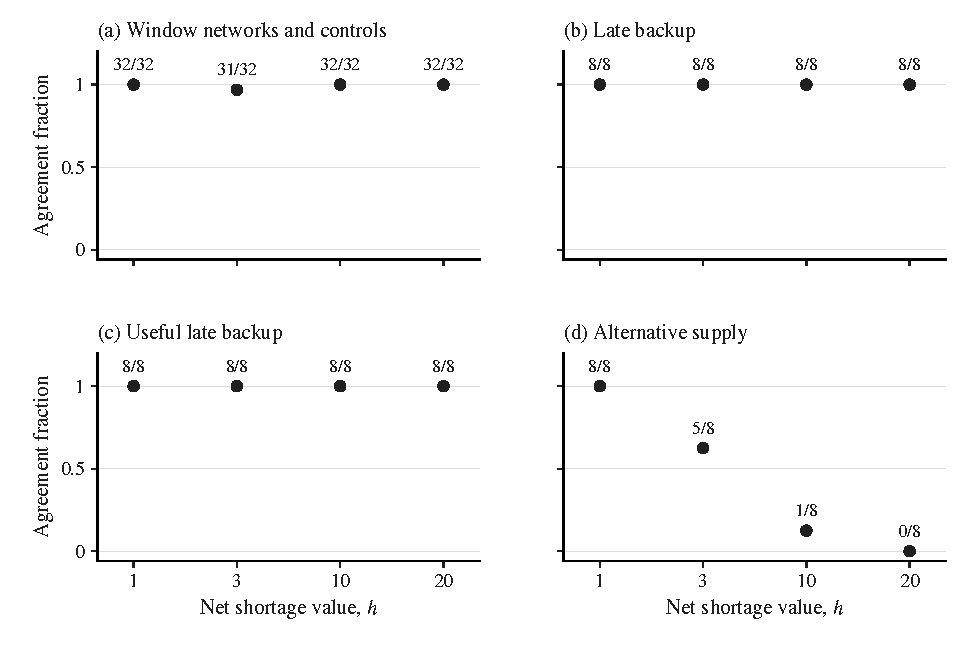
\includegraphics[width=\linewidth]{figures/window_agreement.pdf}\caption{Agreement between the single-buyer window prediction and network truthful qualification in the design sensitivity cases. Points show the fraction of cases that agree at each tested shortage value; labels give the corresponding counts. The combined group contains 24 window networks and eight boundary controls; each comparison regime contains eight networks. All 19 disagreements occur where at least one single-buyer assumption fails.}\label{fig:window}
\ifprovenance\par\scriptsize Source SHA-256: \texttt{99c1b064b04e7cc65a97620b8f94d44ff6a27ff3eeb0841f7ac9a62497613763}\fi\par\end{figure}

\endgroup
% End figure1.tex

\clearpage
\section{Revision audit and additional source review}
The saved-ledger audit compares actions numerically without a tolerance and checks result-bound progress-file hashes. It finds 24 positive backup and primary-delivery contrasts in each set of window networks, 1,120 identical correct-belief action comparisons per set, zero newly accepted orders due during the known outage, and zero post-notice reliance shortfall. Design aggregate results and saved actions supply that part of the comparison. Pre-horizon shortfall remains separately recorded.

Jin et al.'s full online article was supplied and read on 13 November 2026. The closest overlap is Section 5.3, Table 3 and Corollary 1: underestimation can suppress backup in an intermediate inventory range. The model in Section 4.3 supplies backup immediately and charges production-linked quantities; it contains no qualification lag or mandatory post-recovery delivery stream. The article does not model supplier reporting payoffs or the schedule/belief decomposition. The comparison is based on the published main article. The earlier abstract-only status is superseded for the main article.

Demirel et al.'s published main article was also supplied and read in full on 13 November 2026 (pp.~533--551). Section~3 specifies complete information, zero delivery lead times and backlog catch-up. Proposition~4 establishes buyer harm from contingent supplier pricing. Section~6.3 treats deterministic recovery, without a reporting/exposure clock. The comparison is based on the published main article. This supersedes its earlier abstract-only status.

The article's analytical parameter plot evaluates its displayed closed-form inequalities. It generates no network trajectory, interval or test. Supplier-confirmation workflow citations were checked against SAP's official documentation.
\subsection{Saved-path basis for the family breakdown}
Table~\ref{tab:saved_balance} reports the paired balance used in Section~\ref{sec:results}. Here $\widetilde u$ is false-minus-truthful lost demand and $\widetilde E$ is truthful-minus-false terminal stock of the critical part and its finished product. Saved production consumes one critical input per finished output, and these window paths use no spot supply. All displayed paths satisfy $\Delta D=b-\widetilde u-\widetilde E$ within the existing accounting tolerance. 
The Distribution-family channel audit compares saved $C_{01}$ and $C_{11}$ ledgers field by field. Within each pair, total primary deliveries and lost sales are equal. Every aggregate operating-cost component is also equal except transport cost; its difference accounts for the entire interaction. In the pair with positive interaction, lost-sale charges move between periods and cancel in the total. Opening retail stock serves local demand before arrivals. These accounting observations do not isolate a causal effect of stock placement or network family.

% Begin saved_balance_table.tex
% Sources: f1eef2f55a744295094897ce70a38f5b738ac3e41def05b6d53439fd0a41687b, 8d32d1127ecd229475305361a3bbb9fc434e2422c4057bfdd1120b4ead800040, 11639536c750b1d85fedc763be1fc67f781a8cdc75611d02d2f5d19ba35986be, c6c9056671382246ea5ad56855731f9f5f054f628ba01faf198ce14758721bab
\begingroup\small\renewcommand{\thetable}{F1}
\begin{longtable}{p{4.3cm}rrrr}
\caption{Saved delivery balances for confirmation window networks.}\label{tab:saved_balance}\\
\toprule
Network & $b$ & $\widetilde u$ & $\widetilde E$ & $\Delta D$\\\midrule
\endfirsthead
Network & $b$ & $\widetilde u$ & $\widetilde E$ & $\Delta D$\\\midrule
\endhead\bottomrule\endfoot
serial-small-0 & \sr{case0_b} & \sr{case0_extra_lost} & \sr{case0_truth_minus_false_terminal_critical_equivalent} & \sr{case0_delta_d} \\
serial-small-1 & \sr{case1_b} & \sr{case1_extra_lost} & \sr{case1_truth_minus_false_terminal_critical_equivalent} & \sr{case1_delta_d} \\
serial-small-2 & \sr{case2_b} & \sr{case2_extra_lost} & \sr{case2_truth_minus_false_terminal_critical_equivalent} & \sr{case2_delta_d} \\
serial-large-0 & \sr{case3_b} & \sr{case3_extra_lost} & \sr{case3_truth_minus_false_terminal_critical_equivalent} & \sr{case3_delta_d} \\
serial-large-1 & \sr{case4_b} & \sr{case4_extra_lost} & \sr{case4_truth_minus_false_terminal_critical_equivalent} & \sr{case4_delta_d} \\
assembly-small-0 & \sr{case5_b} & \sr{case5_extra_lost} & \sr{case5_truth_minus_false_terminal_critical_equivalent} & \sr{case5_delta_d} \\
assembly-small-1 & \sr{case6_b} & \sr{case6_extra_lost} & \sr{case6_truth_minus_false_terminal_critical_equivalent} & \sr{case6_delta_d} \\
assembly-large-0 & \sr{case7_b} & \sr{case7_extra_lost} & \sr{case7_truth_minus_false_terminal_critical_equivalent} & \sr{case7_delta_d} \\
assembly-large-1 & \sr{case8_b} & \sr{case8_extra_lost} & \sr{case8_truth_minus_false_terminal_critical_equivalent} & \sr{case8_delta_d} \\
assembly-large-2 & \sr{case9_b} & \sr{case9_extra_lost} & \sr{case9_truth_minus_false_terminal_critical_equivalent} & \sr{case9_delta_d} \\
distribution-small-0 & \sr{case10_b} & \sr{case10_extra_lost} & \sr{case10_truth_minus_false_terminal_critical_equivalent} & \sr{case10_delta_d} \\
distribution-small-1 & \sr{case11_b} & \sr{case11_extra_lost} & \sr{case11_truth_minus_false_terminal_critical_equivalent} & \sr{case11_delta_d} \\
distribution-large-0 & \sr{case12_b} & \sr{case12_extra_lost} & \sr{case12_truth_minus_false_terminal_critical_equivalent} & \sr{case12_delta_d} \\
distribution-large-1 & \sr{case13_b} & \sr{case13_extra_lost} & \sr{case13_truth_minus_false_terminal_critical_equivalent} & \sr{case13_delta_d} \\
layered-small-0 & \sr{case14_b} & \sr{case14_extra_lost} & \sr{case14_truth_minus_false_terminal_critical_equivalent} & \sr{case14_delta_d} \\
layered-small-1 & \sr{case15_b} & \sr{case15_extra_lost} & \sr{case15_truth_minus_false_terminal_critical_equivalent} & \sr{case15_delta_d} \\
layered-small-2 & \sr{case16_b} & \sr{case16_extra_lost} & \sr{case16_truth_minus_false_terminal_critical_equivalent} & \sr{case16_delta_d} \\
layered-large-0 & \sr{case17_b} & \sr{case17_extra_lost} & \sr{case17_truth_minus_false_terminal_critical_equivalent} & \sr{case17_delta_d} \\
layered-large-1 & \sr{case18_b} & \sr{case18_extra_lost} & \sr{case18_truth_minus_false_terminal_critical_equivalent} & \sr{case18_delta_d} \\
bypass-route-small-0 & \sr{case19_b} & \sr{case19_extra_lost} & \sr{case19_truth_minus_false_terminal_critical_equivalent} & \sr{case19_delta_d} \\
bypass-route-small-1 & \sr{case20_b} & \sr{case20_extra_lost} & \sr{case20_truth_minus_false_terminal_critical_equivalent} & \sr{case20_delta_d} \\
bypass-route-large-0 & \sr{case21_b} & \sr{case21_extra_lost} & \sr{case21_truth_minus_false_terminal_critical_equivalent} & \sr{case21_delta_d} \\
bypass-route-large-1 & \sr{case22_b} & \sr{case22_extra_lost} & \sr{case22_truth_minus_false_terminal_critical_equivalent} & \sr{case22_delta_d} \\
bypass-route-large-2 & \sr{case23_b} & \sr{case23_extra_lost} & \sr{case23_truth_minus_false_terminal_critical_equivalent} & \sr{case23_delta_d} \\
\end{longtable}\endgroup
% End saved_balance_table.tex


\clearpage
\section{Post-confirmation supplier-margin correction}\label{supp:margin}
The preregistered supplier score used $r=3$ while the buyer paid $p=1$ per primary unit. Interpreting $r=p-c_P$ as an ordinary financial margin would imply $c_P=-2$. This inconsistency was identified after confirmation and corrected by repricing saved deliveries and accepted-order shortfalls . Study source, protocols, allocations, confirmation records and all physical actions were preserved. No trajectory, optimization or new hypothesis test was run for the correction.

The admissible range is $0\le r\le1$, with penalty five, reliance multiplier one and contradiction cost zero in the baseline. The exact affine identity $G_i(r,5)=r\Delta D_i-5\Delta A_i$ supplies the full continuum, including exact network zero crossings. The displayed headline levels are $0,0.25,0.5,0.75,1$. The archived score and original decision are retained in Table~\ref{tab:historical_financial}; its financial conclusion is superseded by the descriptive repricing. The delivery contrast and buyer-harm intervals retain their original three-contrast multiplicity adjustment.

The repricing uses the original 10,000 family-stratified paired bootstrap draws and seed 20261112. It retains the frozen endpoint quantiles 0.00835 and 0.99165, giving pointwise 98.33\% intervals. These are not simultaneous across the continuum. Family, commitment and sensitivity summaries are arithmetic means without inference. The midpoint $r=0.5$ in the article's compact comparison tables is illustrative, not a new empirical calibration.

Independent verification checked exact per-network gains, group summaries, bootstrap endpoints, all sensitivity arms, all belief levels and saved expedite alternatives. Expediting is reselected by comparing $rP-5A-3$ with $rP-5A$; the saved choices remain optimal across the entire admissible range. The positive contradiction-cost arm retains its cost of three, and the no-damages arm retains zero liability. The original discounted-belief objective-recomputation warnings remain unresolved. Verification of financial repricing does not clear them.

The financial analysis used exact affine coefficients, a 0.01 display grid and per-network thresholds. The tables below present its results at their prepared precision.
% Begin historical_table1.tex
% Sources: f1eef2f55a744295094897ce70a38f5b738ac3e41def05b6d53439fd0a41687b, 8d32d1127ecd229475305361a3bbb9fc434e2422c4057bfdd1120b4ead800040, bb0a2208ca1668198cdf09ff091d8cdf37fcbfbe0ec9baf8f5897cc0f51ed224, 7a0c0f4218632c47c75b511f76b8a19df0d0c42bbf06b0cbf77f969ade2a3ce1
\begin{table}[!htbp]\centering\small
\setlength{\tabcolsep}{4pt}\renewcommand{\arraystretch}{1.18}\renewcommand{\thetable}{G1}
\caption{Archived preregistered scoring results before the margin correction. The $r=3$ financial interpretation is superseded.}\label{tab:historical_financial}
\begin{tabular}{>{\raggedright\arraybackslash}p{6.2cm}>{\raggedright\arraybackslash}p{3.8cm}>{\raggedright\arraybackslash}p{3.8cm}}
\toprule
Contrast & Confirmation estimate [interval] & Design estimate [interval] \\
\midrule
\multicolumn{3}{l}{\textit{Joint primary hypothesis}}\\
Backup displacement, b & 10.720 [8.280, 13.100] & 10.720 [8.280, 13.100] \\
Additional primary deliveries, $\Delta D$ & 9.076 [6.690, 11.421] & 9.035 [6.672, 11.367] \\
\addlinespace\multicolumn{3}{l}{\textit{Secondary contrasts}}\\
Additional deliveries: window networks versus comparison networks & 9.401 [6.460, 12.269] & 9.375 [6.456, 12.228] \\
Supplier profitability, G(3,5) & 23.966 [15.552, 32.329] & 23.855 [15.454, 32.223] \\
Buyer harm, C11-C00 & 21.478 [16.838, 26.386] & 21.595 [17.032, 26.468] \\
\bottomrule\end{tabular}

\noindent\footnotesize Equal-family network means. Primary intervals are 95.00\%; secondary intervals are 98.33\% Bonferroni intervals. Both primary lower bounds and all three secondary lower bounds exceed zero, satisfying the prespecified confirmation criteria. Design estimates are descriptive comparisons.\par
\ifprovenance\noindent\scriptsize Source SHA-256: \texttt{f1eef2f55a744295094897ce70a38f5b738ac3e41def05b6d53439fd0a41687b}\par \texttt{8d32d1127ecd229475305361a3bbb9fc434e2422c4057bfdd1120b4ead800040}\par \texttt{bb0a2208ca1668198cdf09ff091d8cdf37fcbfbe0ec9baf8f5897cc0f51ed224}\par \texttt{7a0c0f4218632c47c75b511f76b8a19df0d0c42bbf06b0cbf77f969ade2a3ce1}\par
\fi
\end{table}
% End historical_table1.tex

\clearpage
% Begin margin_sensitivities.tex
% Source SHA-256: eb945f541d609fe28e8dce9b25c8bdc63d3102b000eeb2e52db36757a43d81ab
\begin{table}[!htbp]\centering\small
\setlength{\tabcolsep}{3pt}\renewcommand{\arraystretch}{1.18}\renewcommand{\thetable}{G2}
\caption{All declared design sensitivity arms: arithmetic mean supplier gain over 56 cases.}\label{tab:margin_sens}
\begin{tabular}{>{\raggedright\arraybackslash}p{4.4cm}>{\raggedright\arraybackslash}p{1.8cm}>{\raggedright\arraybackslash}p{1.8cm}>{\raggedright\arraybackslash}p{1.8cm}>{\raggedright\arraybackslash}p{1.8cm}>{\raggedright\arraybackslash}p{1.8cm}}
\toprule
Design arm & $r=\mg{r0}$ & $r=\mg{r1}$ & $r=\mg{r2}$ & $r=\mg{r3}$ & $r=\mg{r4}$ \\
\midrule
Baseline & \mg{sensGrid0_0} & \mg{sensGrid0_1} & \mg{sensGrid0_2} & \mg{sensGrid0_3} & \mg{sensGrid0_4} \\
Backlog + catch-up & \mg{sensGrid1_0} & \mg{sensGrid1_1} & \mg{sensGrid1_2} & \mg{sensGrid1_3} & \mg{sensGrid1_4} \\
Broker spot & \mg{sensGrid2_0} & \mg{sensGrid2_1} & \mg{sensGrid2_2} & \mg{sensGrid2_3} & \mg{sensGrid2_4} \\
Contradiction cost & \mg{sensGrid3_0} & \mg{sensGrid3_1} & \mg{sensGrid3_2} & \mg{sensGrid3_3} & \mg{sensGrid3_4} \\
No damages & \mg{sensGrid4_0} & \mg{sensGrid4_1} & \mg{sensGrid4_2} & \mg{sensGrid4_3} & \mg{sensGrid4_4} \\
Expedite option & \mg{sensGrid5_0} & \mg{sensGrid5_1} & \mg{sensGrid5_2} & \mg{sensGrid5_3} & \mg{sensGrid5_4} \\
Backup price parity & \mg{sensGrid6_0} & \mg{sensGrid6_1} & \mg{sensGrid6_2} & \mg{sensGrid6_3} & \mg{sensGrid6_4} \\
Shortage h=1 & \mg{sensGrid7_0} & \mg{sensGrid7_1} & \mg{sensGrid7_2} & \mg{sensGrid7_3} & \mg{sensGrid7_4} \\
Shortage h=3 & \mg{sensGrid8_0} & \mg{sensGrid8_1} & \mg{sensGrid8_2} & \mg{sensGrid8_3} & \mg{sensGrid8_4} \\
Shortage h=10 & \mg{sensGrid9_0} & \mg{sensGrid9_1} & \mg{sensGrid9_2} & \mg{sensGrid9_3} & \mg{sensGrid9_4} \\
\bottomrule\end{tabular}
\end{table}
% End margin_sensitivities.tex

% Begin margin_beliefs.tex
% Source SHA-256: 4a167dd25743218d59231709e5c75934fc156ae2fe64d65c1bc2e3961f6e4fba
\begin{table}[!htbp]\centering\small
\setlength{\tabcolsep}{3pt}\renewcommand{\arraystretch}{1.18}\renewcommand{\thetable}{G3}
\caption{Discounted-belief design comparison: arithmetic mean gain among window networks.}\label{tab:margin_beliefs}
\begin{tabular}{>{\raggedright\arraybackslash}p{1.5cm}>{\raggedright\arraybackslash}p{2.2cm}>{\raggedright\arraybackslash}p{2.2cm}>{\raggedright\arraybackslash}p{2.2cm}>{\raggedright\arraybackslash}p{2.2cm}>{\raggedright\arraybackslash}p{2.2cm}}
\toprule
$\alpha$ & $r=\mg{r0}$ & $r=\mg{r1}$ & $r=\mg{r2}$ & $r=\mg{r3}$ & $r=\mg{r4}$ \\
\midrule
\db{alpha0} & \mg{dbGrid0_0} & \mg{dbGrid0_1} & \mg{dbGrid0_2} & \mg{dbGrid0_3} & \mg{dbGrid0_4} \\
\db{alpha1} & \mg{dbGrid1_0} & \mg{dbGrid1_1} & \mg{dbGrid1_2} & \mg{dbGrid1_3} & \mg{dbGrid1_4} \\
\db{alpha2} & \mg{dbGrid2_0} & \mg{dbGrid2_1} & \mg{dbGrid2_2} & \mg{dbGrid2_3} & \mg{dbGrid2_4} \\
\db{alpha3} & \mg{dbGrid3_0} & \mg{dbGrid3_1} & \mg{dbGrid3_2} & \mg{dbGrid3_3} & \mg{dbGrid3_4} \\
\db{alpha4} & \mg{dbGrid4_0} & \mg{dbGrid4_1} & \mg{dbGrid4_2} & \mg{dbGrid4_3} & \mg{dbGrid4_4} \\
\bottomrule\end{tabular}
\end{table}
% End margin_beliefs.tex

\clearpage
% Begin margin_critical.tex
% Source SHA-256: 6dcebbb05cbe11e0e20db9faabecf2ab71c5ac30336a7f0bdd8343eef89aecdc
\begin{table}[!htbp]\centering\small
\setlength{\tabcolsep}{3pt}\renewcommand{\arraystretch}{1.18}\renewcommand{\thetable}{G4}
\caption{Critical-penalty categories across all 56 cases in each set.}\label{tab:margin_critical}
\begin{tabular}{>{\raggedright\arraybackslash}p{2.6cm}>{\raggedright\arraybackslash}p{0.7cm}>{\raggedright\arraybackslash}p{1.5cm}>{\raggedright\arraybackslash}p{2cm}>{\raggedright\arraybackslash}p{2cm}>{\raggedright\arraybackslash}p{1.4cm}>{\raggedright\arraybackslash}p{3.8cm}}
\toprule
Set & r & Finite positive range & Penalty-independent positive & Penalty-independent zero & No positive range & Finite min / median / max \\
\midrule
Confirmation & \mg{r0} & \mg{critconfirmation0c0} & \mg{critconfirmation0c1} & \mg{critconfirmation0c2} & \mg{critconfirmation0c3} & --- \\
Confirmation & \mg{r1} & \mg{critconfirmation1c0} & \mg{critconfirmation1c1} & \mg{critconfirmation1c2} & \mg{critconfirmation1c3} & \mg{critconfirmation1s0} / \mg{critconfirmation1s1} / \mg{critconfirmation1s2} \\
Confirmation & \mg{r2} & \mg{critconfirmation2c0} & \mg{critconfirmation2c1} & \mg{critconfirmation2c2} & \mg{critconfirmation2c3} & \mg{critconfirmation2s0} / \mg{critconfirmation2s1} / \mg{critconfirmation2s2} \\
Confirmation & \mg{r3} & \mg{critconfirmation3c0} & \mg{critconfirmation3c1} & \mg{critconfirmation3c2} & \mg{critconfirmation3c3} & \mg{critconfirmation3s0} / \mg{critconfirmation3s1} / \mg{critconfirmation3s2} \\
Confirmation & \mg{r4} & \mg{critconfirmation4c0} & \mg{critconfirmation4c1} & \mg{critconfirmation4c2} & \mg{critconfirmation4c3} & \mg{critconfirmation4s0} / \mg{critconfirmation4s1} / \mg{critconfirmation4s2} \\
Design & \mg{r0} & \mg{critdesign0c0} & \mg{critdesign0c1} & \mg{critdesign0c2} & \mg{critdesign0c3} & --- \\
Design & \mg{r1} & \mg{critdesign1c0} & \mg{critdesign1c1} & \mg{critdesign1c2} & \mg{critdesign1c3} & \mg{critdesign1s0} / \mg{critdesign1s1} / \mg{critdesign1s2} \\
Design & \mg{r2} & \mg{critdesign2c0} & \mg{critdesign2c1} & \mg{critdesign2c2} & \mg{critdesign2c3} & \mg{critdesign2s0} / \mg{critdesign2s1} / \mg{critdesign2s2} \\
Design & \mg{r3} & \mg{critdesign3c0} & \mg{critdesign3c1} & \mg{critdesign3c2} & \mg{critdesign3c3} & \mg{critdesign3s0} / \mg{critdesign3s1} / \mg{critdesign3s2} \\
Design & \mg{r4} & \mg{critdesign4c0} & \mg{critdesign4c1} & \mg{critdesign4c2} & \mg{critdesign4c3} & \mg{critdesign4s0} / \mg{critdesign4s1} / \mg{critdesign4s2} \\
\bottomrule\end{tabular}
\par\medskip\parbox{\linewidth}{\footnotesize Threshold summaries include only cases with a strictly positive profitable penalty range. A zero-gain penalty of zero remains defined when the shortfall contrast is nonzero. Zero shortfall makes the threshold undefined; the gain category then applies.}
\end{table}
% End margin_critical.tex


\clearpage
\section{Controlled commitment comparison and incentive-map provenance}\label{supp:paired}
The post-confirmation comparison changes only the backup commitment rule in each of the \pc{n} public design window networks. Each rule receives the four schedule-belief cells and the fractional-belief levels. Qualification remains optional; every case and level is retained. The ordinary margin grid has \pc{rCount} levels from \pc{rMin} to \pc{rMax} in steps of \pc{rStep}; \pc{kCount} penalty levels span \pc{kappaMin} to \pc{kappaMax}. Every effect is referenced to truthful $C_{00}$ under the same commitment. These are descriptive comparisons with no new confirmatory test.

The execution manifest SHA-256 is\par\noindent{\small\texttt{\pc{manifestHash}}}\par Its limits are \pc{cappaths} paths, including at most \pc{capnew_paths} new paths and \pc{capmaximum_mip_phases} new MIPs, \pc{capwall_seconds} seconds, \pc{cappeak_rss_mib} MiB, and \pc{capretries} retries. The run completed all \pc{runcompleted_paths} paths using \pc{runmip_phases} MIPs in \pc{runelapsed_seconds} seconds with peak memory \pc{runpeak_rss_mib} MiB. The independent verifier ran after completion and passed without new solves. The result SHA-256 is\par\noindent{\small\texttt{\pc{resultHash}}}\par

Table~\ref{tab:paired_networks} reports every network. F and H denote finite and through-horizon commitments. A switch indicator of one means non-positive finite gain becomes positive horizon gain, using the manifest's numerical sign rule. Thresholds are tested grid levels without interpolation; ``none'' means no positive gain on that grid. The accompanying \texttt{NETWORK\_GRID.csv}, \texttt{PAIRED\_GRID.csv}, \texttt{NETWORK\_THRESHOLDS.csv} and \texttt{GAIN\_SWITCH\_COUNTS.md} retain all beliefs, margins, penalties, signs and both switch directions. The \texttt{group\_grid} and \texttt{paired\_group\_grid} arrays retain both arithmetic and equal-family means. The included \path{paper/paired_commitment_r1/study_report/SOURCE_MAP.json} maps the CSV reports to \path{paper/paired_commitment_r1/study_execution/descriptive_report.json} by source hash, array and row. The source files preserve all four-cell decompositions and the cases with negative paired gain changes.
\clearpage% Begin paired_networks.tex
% Source SHA-256: e2cab9704d002158e0b7c75a1ce86356b5124c1949445437ce2ba68e3de1968f
\begingroup\small\setlength{\tabcolsep}{3.5pt}\renewcommand{\arraystretch}{1.14}
\renewcommand{\thetable}{H1}\setlength{\LTcapwidth}{\linewidth}
\begin{longtable}{lcccrrr}
\caption{Every public design window network at $\kappa=\pc{kappa}$. Thresholds give the lowest tested positive-gain margin under full belief. The final columns indicate a non-positive-to-positive switch at $r=\pc{rHalf}$.}\label{tab:paired_networks}\\
\toprule Network & Truthful $q$ F/H & Lowest $r$ F & Lowest $r$ H & $\alpha=\pc{alpha2}$ & $\alpha=\pc{alpha3}$ & $\alpha=\pc{alpha4}$\\\midrule\endfirsthead
\toprule Network & Truthful $q$ F/H & Lowest $r$ F & Lowest $r$ H & $\alpha=\pc{alpha2}$ & $\alpha=\pc{alpha3}$ & $\alpha=\pc{alpha4}$\\\midrule\endhead
\bottomrule\endfoot
assembly-large-0 & \pc{q0finite} / \pc{q0horizon} & \pc{th0finite} & \pc{th0horizon} & \pc{sw00.5} & \pc{sw00.75} & \pc{sw01}\\
assembly-large-1 & \pc{q1finite} / \pc{q1horizon} & \pc{th1finite} & \pc{th1horizon} & \pc{sw10.5} & \pc{sw10.75} & \pc{sw11}\\
assembly-large-2 & \pc{q2finite} / \pc{q2horizon} & \pc{th2finite} & \pc{th2horizon} & \pc{sw20.5} & \pc{sw20.75} & \pc{sw21}\\
assembly-small-0 & \pc{q3finite} / \pc{q3horizon} & \pc{th3finite} & \pc{th3horizon} & \pc{sw30.5} & \pc{sw30.75} & \pc{sw31}\\
assembly-small-1 & \pc{q4finite} / \pc{q4horizon} & \pc{th4finite} & \pc{th4horizon} & \pc{sw40.5} & \pc{sw40.75} & \pc{sw41}\\
distribution-large-0 & \pc{q5finite} / \pc{q5horizon} & \pc{th5finite} & \pc{th5horizon} & \pc{sw50.5} & \pc{sw50.75} & \pc{sw51}\\
distribution-large-1 & \pc{q6finite} / \pc{q6horizon} & \pc{th6finite} & \pc{th6horizon} & \pc{sw60.5} & \pc{sw60.75} & \pc{sw61}\\
distribution-small-0 & \pc{q7finite} / \pc{q7horizon} & \pc{th7finite} & \pc{th7horizon} & \pc{sw70.5} & \pc{sw70.75} & \pc{sw71}\\
distribution-small-1 & \pc{q8finite} / \pc{q8horizon} & \pc{th8finite} & \pc{th8horizon} & \pc{sw80.5} & \pc{sw80.75} & \pc{sw81}\\
layered-large-0 & \pc{q9finite} / \pc{q9horizon} & \pc{th9finite} & \pc{th9horizon} & \pc{sw90.5} & \pc{sw90.75} & \pc{sw91}\\
layered-large-1 & \pc{q10finite} / \pc{q10horizon} & \pc{th10finite} & \pc{th10horizon} & \pc{sw100.5} & \pc{sw100.75} & \pc{sw101}\\
layered-small-0 & \pc{q11finite} / \pc{q11horizon} & \pc{th11finite} & \pc{th11horizon} & \pc{sw110.5} & \pc{sw110.75} & \pc{sw111}\\
layered-small-1 & \pc{q12finite} / \pc{q12horizon} & \pc{th12finite} & \pc{th12horizon} & \pc{sw120.5} & \pc{sw120.75} & \pc{sw121}\\
layered-small-2 & \pc{q13finite} / \pc{q13horizon} & \pc{th13finite} & \pc{th13horizon} & \pc{sw130.5} & \pc{sw130.75} & \pc{sw131}\\
bypass-large-0 & \pc{q14finite} / \pc{q14horizon} & \pc{th14finite} & \pc{th14horizon} & \pc{sw140.5} & \pc{sw140.75} & \pc{sw141}\\
bypass-large-1 & \pc{q15finite} / \pc{q15horizon} & \pc{th15finite} & \pc{th15horizon} & \pc{sw150.5} & \pc{sw150.75} & \pc{sw151}\\
bypass-large-2 & \pc{q16finite} / \pc{q16horizon} & \pc{th16finite} & \pc{th16horizon} & \pc{sw160.5} & \pc{sw160.75} & \pc{sw161}\\
bypass-small-0 & \pc{q17finite} / \pc{q17horizon} & \pc{th17finite} & \pc{th17horizon} & \pc{sw170.5} & \pc{sw170.75} & \pc{sw171}\\
bypass-small-1 & \pc{q18finite} / \pc{q18horizon} & \pc{th18finite} & \pc{th18horizon} & \pc{sw180.5} & \pc{sw180.75} & \pc{sw181}\\
serial-large-0 & \pc{q19finite} / \pc{q19horizon} & \pc{th19finite} & \pc{th19horizon} & \pc{sw190.5} & \pc{sw190.75} & \pc{sw191}\\
serial-large-1 & \pc{q20finite} / \pc{q20horizon} & \pc{th20finite} & \pc{th20horizon} & \pc{sw200.5} & \pc{sw200.75} & \pc{sw201}\\
serial-small-0 & \pc{q21finite} / \pc{q21horizon} & \pc{th21finite} & \pc{th21horizon} & \pc{sw210.5} & \pc{sw210.75} & \pc{sw211}\\
serial-small-1 & \pc{q22finite} / \pc{q22horizon} & \pc{th22finite} & \pc{th22horizon} & \pc{sw220.5} & \pc{sw220.75} & \pc{sw221}\\
serial-small-2 & \pc{q23finite} / \pc{q23horizon} & \pc{th23finite} & \pc{th23horizon} & \pc{sw230.5} & \pc{sw230.75} & \pc{sw231}\\
\end{longtable}\endgroup
% End paired_networks.tex


The incentive map reprices saved confirmation outcomes using the exact rational ratio of the equal-family delivery and shortfall coefficients. Points on each line have zero mean gain; the positive region is strictly below it. The prepared plot is included at \path{manuscript/figures/profitability_combined.pdf}.

\clearpage
\section{Ex ante commitment comparison}\label{app:exante}
The post-confirmation comparison uses \xa{n} public design window networks and both commitment rules. The prior and reporting-likelihood grid is declared in Section~\ref{sec:exante_design}. Short types report minor, long types do so with the externally specified probability $\beta$, and minor notices induce the Bayes-consistent posterior. All probability cells, exact ties, cost decompositions and conditional supplier gains are retained. The article reports equal-family means; Figure~\ref{fig:exante_arithmetic} supplies the arithmetic panel.

\begin{figure}[!htbp]\centering
\renewcommand{\thefigure}{I1}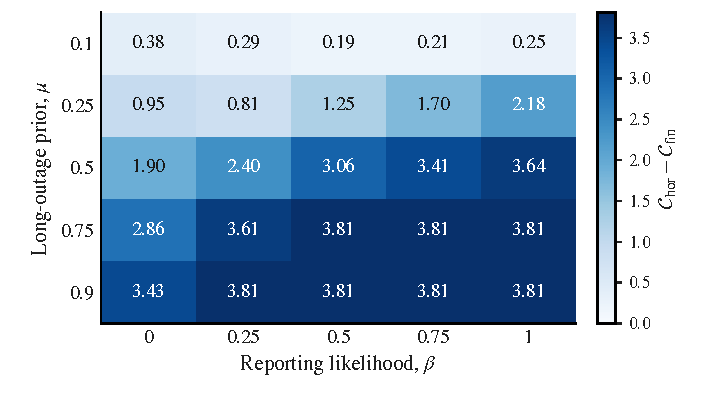
\includegraphics[width=.77\linewidth]{figures/ex_ante_arithmetic.pdf}
\caption{Arithmetic network mean of through-horizon minus finite expected operating cost on the complete tested grid. Positive values favor finite commitment.}\label{fig:exante_arithmetic}
\end{figure}

The article defines a positive break-even discount $\delta^*=\mathcal C_{\mathrm{hor}}-\mathcal C_{\mathrm{fin}}$. The saved output's fee premium has the opposite sign: it is the maximum unconditional additional fee for the longer contract. No qualification-contingent price change is evaluated. The complete \texttt{network\_contract\_grid.csv}, \texttt{paired\_grid.csv} and \texttt{aggregate\_grid.csv} retain the branch costs, precaution and misreporting components, exact saved-decimal arithmetic, preferred contracts and supplier-incentive diagnostics. The scientific report grids and their locators are included in \path{paper/ex_ante_contract_r1/report/}, including \texttt{SOURCE\_MAP.json} and \texttt{RESULT\_SOURCE\_MAP.json}. No network-equilibrium or new hypothesis test is performed.

The completed continuation combines \xa{cachedPaths} cached paths with \xa{newPaths} newly solved paths, covering all \xa{paths} paths with \xa{mips} new MIPs in \xa{seconds} seconds. Its cap was \xa{mipCap} new MIPs and \xa{wallCap} seconds; there were no failures or automatic retries. Independent verification replayed all saved actions and recomputed the reporting tables without solving. The two earlier attempts stopped: the first stopped after a solver time limit with a computer interruption reported by the authors; the second exhausted its total wall cap. The continuation reused complete paths and restarted only unfinished work. The historical warning disposition in Supplement~G remains unchanged.

\noindent Manifest SHA-256:\par\noindent\texttt{\xa{manifestHash}}\par
\noindent Result SHA-256:\par\noindent\texttt{\xa{resultHash}}\par
\noindent Verification SHA-256:\par\noindent\texttt{\xa{verificationHash}}\par
\clearpage% Begin ex_ante_tables.tex
% Source SHA-256: de8810d45034f4d665cd18eb6cdd9892d9424abdfe7e978ec00daeb48b625c40
\renewcommand{\thetable}{I1}
\begingroup\small\setlength{\tabcolsep}{4pt}\begin{longtable}{rrrrrrrr}
\caption{Equal-family means: complete ex ante probability grid. Cost difference is through-horizon minus finite and equals the break-even up-front discount. Counts select finite at equality.}\\
\toprule $\mu$ & $\beta$ & Finite cost & Horizon cost & Difference & Finite $n$ & Horizon $n$ & Ties\\\midrule
\endfirsthead
\toprule $\mu$ & $\beta$ & Finite cost & Horizon cost & Difference & Finite $n$ & Horizon $n$ & Ties\\\midrule
\endhead\bottomrule\endfoot
0.10 & 0.00 & 30.997 & 31.378 & 0.381 & 24 & 0 & 0\\
0.10 & 0.25 & 31.586 & 31.872 & 0.286 & 24 & 0 & 0\\
0.10 & 0.50 & 32.171 & 32.366 & 0.194 & 24 & 0 & 0\\
0.10 & 0.75 & 32.658 & 32.860 & 0.201 & 24 & 0 & 0\\
0.10 & 1.00 & 33.112 & 33.354 & 0.241 & 24 & 0 & 19\\
0.25 & 0.00 & 33.470 & 34.422 & 0.952 & 24 & 0 & 0\\
0.25 & 0.25 & 34.855 & 35.657 & 0.802 & 24 & 0 & 0\\
0.25 & 0.50 & 35.643 & 36.878 & 1.235 & 24 & 0 & 0\\
0.25 & 0.75 & 36.132 & 37.821 & 1.689 & 24 & 0 & 0\\
0.25 & 1.00 & 36.316 & 38.501 & 2.185 & 24 & 0 & 5\\
0.50 & 0.00 & 37.592 & 39.497 & 1.905 & 24 & 0 & 0\\
0.50 & 0.25 & 39.367 & 41.763 & 2.396 & 24 & 0 & 0\\
0.50 & 0.50 & 39.718 & 42.783 & 3.065 & 24 & 0 & 0\\
0.50 & 0.75 & 39.761 & 43.165 & 3.404 & 24 & 0 & 0\\
0.50 & 1.00 & 39.761 & 43.406 & 3.645 & 24 & 0 & 0\\
0.75 & 0.00 & 41.714 & 44.571 & 2.857 & 24 & 0 & 0\\
0.75 & 0.25 & 42.799 & 46.405 & 3.607 & 24 & 0 & 0\\
0.75 & 0.50 & 42.800 & 46.609 & 3.809 & 24 & 0 & 0\\
0.75 & 0.75 & 42.801 & 46.610 & 3.809 & 24 & 0 & 0\\
0.75 & 1.00 & 42.802 & 46.611 & 3.809 & 24 & 0 & 0\\
0.90 & 0.00 & 44.188 & 47.616 & 3.428 & 24 & 0 & 0\\
0.90 & 0.25 & 44.622 & 48.431 & 3.809 & 24 & 0 & 0\\
0.90 & 0.50 & 44.623 & 48.433 & 3.809 & 24 & 0 & 0\\
0.90 & 0.75 & 44.625 & 48.434 & 3.809 & 24 & 0 & 0\\
0.90 & 1.00 & 44.626 & 48.435 & 3.809 & 24 & 0 & 0\\
\end{longtable}\endgroup
\renewcommand{\thetable}{I2}
\begingroup\small\setlength{\tabcolsep}{4pt}\begin{longtable}{rrrrrrrr}
\caption{Arithmetic network means: complete ex ante probability grid. Cost difference is through-horizon minus finite and equals the break-even up-front discount. Counts select finite at equality.}\\
\toprule $\mu$ & $\beta$ & Finite cost & Horizon cost & Difference & Finite $n$ & Horizon $n$ & Ties\\\midrule
\endfirsthead
\toprule $\mu$ & $\beta$ & Finite cost & Horizon cost & Difference & Finite $n$ & Horizon $n$ & Ties\\\midrule
\endhead\bottomrule\endfoot
0.10 & 0.00 & 31.334 & 31.715 & 0.381 & 24 & 0 & 0\\
0.10 & 0.25 & 31.926 & 32.212 & 0.286 & 24 & 0 & 0\\
0.10 & 0.50 & 32.515 & 32.709 & 0.195 & 24 & 0 & 0\\
0.10 & 0.75 & 33.001 & 33.206 & 0.205 & 24 & 0 & 0\\
0.10 & 1.00 & 33.455 & 33.704 & 0.249 & 24 & 0 & 19\\
0.25 & 0.00 & 33.851 & 34.803 & 0.952 & 24 & 0 & 0\\
0.25 & 0.25 & 35.240 & 36.046 & 0.806 & 24 & 0 & 0\\
0.25 & 0.50 & 36.025 & 37.274 & 1.249 & 24 & 0 & 0\\
0.25 & 0.75 & 36.513 & 38.214 & 1.701 & 24 & 0 & 0\\
0.25 & 1.00 & 36.696 & 38.879 & 2.184 & 24 & 0 & 5\\
0.50 & 0.00 & 38.046 & 39.951 & 1.904 & 24 & 0 & 0\\
0.50 & 0.25 & 39.821 & 42.225 & 2.404 & 24 & 0 & 0\\
0.50 & 0.50 & 40.169 & 43.230 & 3.061 & 24 & 0 & 0\\
0.50 & 0.75 & 40.211 & 43.616 & 3.405 & 24 & 0 & 0\\
0.50 & 1.00 & 40.212 & 43.855 & 3.643 & 24 & 0 & 0\\
0.75 & 0.00 & 42.241 & 45.098 & 2.857 & 24 & 0 & 0\\
0.75 & 0.25 & 43.324 & 46.931 & 3.607 & 24 & 0 & 0\\
0.75 & 0.50 & 43.325 & 47.134 & 3.809 & 24 & 0 & 0\\
0.75 & 0.75 & 43.326 & 47.135 & 3.809 & 24 & 0 & 0\\
0.75 & 1.00 & 43.327 & 47.136 & 3.809 & 24 & 0 & 0\\
0.90 & 0.00 & 44.758 & 48.186 & 3.428 & 24 & 0 & 0\\
0.90 & 0.25 & 45.192 & 49.001 & 3.809 & 24 & 0 & 0\\
0.90 & 0.50 & 45.194 & 49.002 & 3.809 & 24 & 0 & 0\\
0.90 & 0.75 & 45.195 & 49.004 & 3.809 & 24 & 0 & 0\\
0.90 & 1.00 & 45.196 & 49.005 & 3.809 & 24 & 0 & 0\\
\end{longtable}\endgroup
% End ex_ante_tables.tex

\clearpage
\subsection{Unconditional fixed concession}
The hypothetical date-zero concession is $\delta=\fd{delta}$, independent of backup qualification, volume, the realized outage and reporting. For every network and probability pair,
\[
 \Delta_i^\delta(\mu,\beta)=\Delta_i(\mu,\beta)-\delta,
 \qquad \delta_i^*(\mu,\beta)=\Delta_i(\mu,\beta).
\]
Through-horizon commitment is selected when the adjusted difference is strictly negative; finite commitment is selected at equality. The adjustment is made to buyer cost only. Conditional supplier gains, all physical paths, the probability grid and the Bayesian posterior are unchanged. These are deterministic transformations of the existing post-confirmation exploratory data, with no new simulation, equilibrium calculation, intervals or significance tests.

Table I3 separates preferences based on the equal-family mean from the individual-network counts in Table I4. The concession makes through-horizon preferable in \fd{eq_horizon_after} of \fd{eq_cells} mean comparisons and \fd{horizon_after} of \fd{network_comparisons} individual comparisons. All \fd{switches} individual switches are from finite to through-horizon; the \fd{finite_after} retained finite choices include \fd{ties_after} exact ties. The underlying \texttt{NETWORK\_PREFERENCES.csv} retains each network's original gap, adjusted gap, both preferences, switch indicator and break-even discount. \texttt{AGGREGATE\_PREFERENCES.csv} retains both weighting schemes and all probability combinations. No interpolation is used.

At $\mu=\xa{mu2}$ and $\beta=\xa{beta0}$, the equal-family gap changes from \fd{low_original} to \fd{low_adjusted} after adjustment. At $\beta=\xa{beta4}$, the corresponding values are \fd{high_original} and \fd{high_adjusted}. The exact values and source pointers for both examples are in \texttt{NUMERICAL\_VERIFICATION.json}. Selection is computed with rational arithmetic from the unrounded saved fields, never from displayed values.

The source is \path{paper/ex_ante_contract_r1/study_execution_r3/descriptive_report.json}, with the result and verification hashes recorded above. The unconditional concession is recorded in \path{paper/fixed_discount_r1/NEW_NUMBER_SOURCES.json}. The prepared outputs for Figure~\ref{fig:ex_ante}, numerical verification and source locators are included in \path{paper/fixed_discount_r1/}, with \texttt{NUMERICAL\_VERIFICATION.json}, \texttt{NEW\_NUMBER\_SOURCES.json}, \texttt{TABLE\_SOURCES.json} and \texttt{FIGURE\_SOURCES.json}. Original evidence remains unchanged.
% Begin fixed_discount_tables.tex
% Source SHA-256: de8810d45034f4d665cd18eb6cdd9892d9424abdfe7e978ec00daeb48b625c40; discount specification: 06e8a77742037508c31046219c09ff4b7b29692fe3bc7b852dfd278f2fe3f990
\renewcommand{\thetable}{I3}
\begingroup\small\setlength{\tabcolsep}{5pt}\begin{longtable}{rr rr cc}
\caption{Equal-family preferences before and after the unconditional concession. $F$ denotes finite and $H$ through-horizon; both columns use exact unrounded mean costs.}\\
\toprule $\mu$ & $\beta$ & Original gap & Adjusted gap & Before & After\\\midrule
\endfirsthead
\toprule $\mu$ & $\beta$ & Original gap & Adjusted gap & Before & After\\\midrule
\endhead\bottomrule\endfoot
0.10 & 0.00 & +0.381 & -1.619 & F & H\\
0.10 & 0.25 & +0.286 & -1.714 & F & H\\
0.10 & 0.50 & +0.194 & -1.806 & F & H\\
0.10 & 0.75 & +0.201 & -1.799 & F & H\\
0.10 & 1.00 & +0.241 & -1.759 & F & H\\
0.25 & 0.00 & +0.952 & -1.048 & F & H\\
0.25 & 0.25 & +0.802 & -1.198 & F & H\\
0.25 & 0.50 & +1.235 & -0.765 & F & H\\
0.25 & 0.75 & +1.689 & -0.311 & F & H\\
0.25 & 1.00 & +2.185 & +0.185 & F & F\\
0.50 & 0.00 & +1.905 & -0.096 & F & H\\
0.50 & 0.25 & +2.396 & +0.396 & F & F\\
0.50 & 0.50 & +3.065 & +1.065 & F & F\\
0.50 & 0.75 & +3.404 & +1.404 & F & F\\
0.50 & 1.00 & +3.645 & +1.645 & F & F\\
0.75 & 0.00 & +2.857 & +0.857 & F & F\\
0.75 & 0.25 & +3.607 & +1.607 & F & F\\
0.75 & 0.50 & +3.809 & +1.809 & F & F\\
0.75 & 0.75 & +3.809 & +1.809 & F & F\\
0.75 & 1.00 & +3.809 & +1.809 & F & F\\
0.90 & 0.00 & +3.428 & +1.428 & F & F\\
0.90 & 0.25 & +3.809 & +1.809 & F & F\\
0.90 & 0.50 & +3.809 & +1.809 & F & F\\
0.90 & 0.75 & +3.809 & +1.809 & F & F\\
0.90 & 1.00 & +3.809 & +1.809 & F & F\\
\end{longtable}\endgroup
\renewcommand{\thetable}{I4}
\begingroup\small\setlength{\tabcolsep}{5pt}\begin{longtable}{rr rrrrr}
\caption{Individual-network preference counts on the same grid. Ties choose finite. The undiscounted comparison chooses finite in every network; switches here are from finite to through-horizon.}\\
\toprule $\mu$ & $\beta$ & Original ties & Finite after & Horizon after & Ties after & Switches\\\midrule
\endfirsthead
\toprule $\mu$ & $\beta$ & Original ties & Finite after & Horizon after & Ties after & Switches\\\midrule
\endhead\bottomrule\endfoot
0.10 & 0.00 & 0 & 0 & 24 & 0 & 24\\
0.10 & 0.25 & 0 & 0 & 24 & 0 & 24\\
0.10 & 0.50 & 0 & 0 & 24 & 0 & 24\\
0.10 & 0.75 & 0 & 0 & 24 & 0 & 24\\
0.10 & 1.00 & 19 & 1 & 23 & 1 & 23\\
0.25 & 0.00 & 0 & 0 & 24 & 0 & 24\\
0.25 & 0.25 & 0 & 0 & 24 & 0 & 24\\
0.25 & 0.50 & 0 & 4 & 20 & 0 & 20\\
0.25 & 0.75 & 0 & 12 & 12 & 0 & 12\\
0.25 & 1.00 & 5 & 14 & 10 & 0 & 10\\
0.50 & 0.00 & 0 & 12 & 12 & 7 & 12\\
0.50 & 0.25 & 0 & 13 & 11 & 0 & 11\\
0.50 & 0.50 & 0 & 19 & 5 & 0 & 5\\
0.50 & 0.75 & 0 & 21 & 3 & 0 & 3\\
0.50 & 1.00 & 0 & 24 & 0 & 0 & 0\\
0.75 & 0.00 & 0 & 24 & 0 & 0 & 0\\
0.75 & 0.25 & 0 & 24 & 0 & 0 & 0\\
0.75 & 0.50 & 0 & 24 & 0 & 0 & 0\\
0.75 & 0.75 & 0 & 24 & 0 & 0 & 0\\
0.75 & 1.00 & 0 & 24 & 0 & 0 & 0\\
0.90 & 0.00 & 0 & 24 & 0 & 0 & 0\\
0.90 & 0.25 & 0 & 24 & 0 & 0 & 0\\
0.90 & 0.50 & 0 & 24 & 0 & 0 & 0\\
0.90 & 0.75 & 0 & 24 & 0 & 0 & 0\\
0.90 & 1.00 & 0 & 24 & 0 & 0 & 0\\
\end{longtable}\endgroup
% End fixed_discount_tables.tex

\end{document}

